% !TEX root = ../Elements.tex
% Greek and English text last checked 17/03/2013
%%%%%%
% BOOK 5
%%%%%%
\pdfbookmark[0]{Book 5}{book5}
\pagestyle{empty}
\begin{center}
{\Huge ELEMENTS BOOK 5}\\
\spa\spa\spa
{\huge\it Proportion\symbolfootnote[2]{The theory of proportion set out in this
book is generally attributed to Eudoxus of Cnidus. The novel feature of this theory is its ability to deal with irrational magnitudes, which had hitherto been
a major stumbling block for Greek mathematicians. Throughout the footnotes in this
book, $\alpha$, $\beta$, $\gamma$, {\rm etc.}, denote general (possibly irrational) magnitudes, whereas $m$, $n$, $l$,  {\rm etc.}, denote
positive integers.}}
\end{center}
%\vspace{3cm}
%% Removed epsf size command
%\centerline{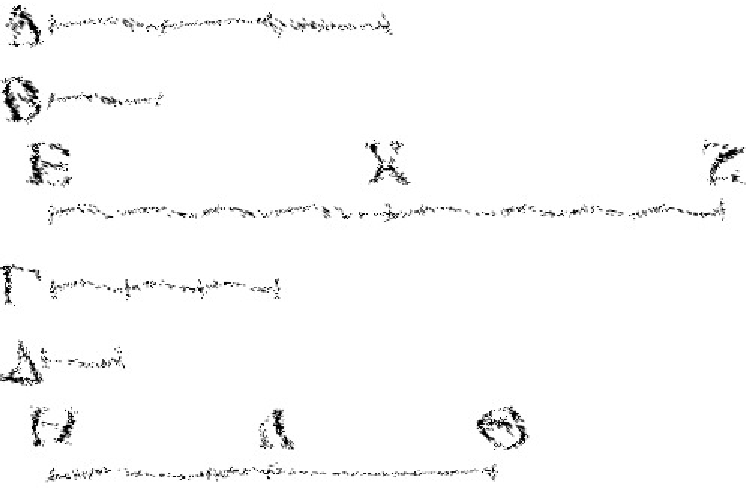
\includegraphics[width=0.8\textwidth]{Book05/front.pdf}}
\newpage

%%%%%%%
% Definitions
%%%%%%%
\pdfbookmark[1]{Definitions}{def5}
\pagestyle{fancy}
\cfoot{\gr{ }}
\lhead{\large\gr{ΣΤΟΙΘΕΙΩΝ  {5}.}}
\rhead{\large ELEMENTS BOOK 5}
\begin{Parallel}{}{} 
\ParallelLText{
\begin{center}
\large{\gr{ὍΟροι}.}
\end{center}\vspace*{-7pt}

\ggn{1}.~\gr{Μέρος ἐστὶ μέγεθος μεγέθους τὸ ὸέλασσον τοῦ μείζονος,
ὅταν καταμετρῆ| τὸ μεῖζον.}

\ggn{2}.~\gr{Πολλαπλάσιον δὲ τὸ μεῖζον τοῦ ἐλάττονος, ὅταν καταμετρῆται ὑπὸ τοῦ ἐλάττονος.}

\ggn{3}.~\gr{Λόγος ἐστὶ δύο μεγεθῶν ὁμογενῶν ἡ κατὰ πηλικότητά
ποια σθέσις.}

\ggn{4}.~\gr{Λόγον ἔχειν πρὸςὸάλληλα μεγέθη λέγεται, ὁὰ δύναται
πολλαπλασιαζόμενα ἀλλήλων ὑπερέθειν.}

\ggn{5}.~\gr{Ἐν τῷ αὐτῷ λόγῳ μεγέθη λέγεται εὸῖναι πρῶτον πρὸς
δεύτερον καὶ τρίτον πρὸς τέταρτον, ὅταν τὰ τοῦ πρώτου καί
τρίτου ἰσάκις πολλαπλάσια τῶν τοῦ δευτέρου καὶ τετάρτου
ἰσάκις πολλαπλασίων καθὸ ὁποιονοῦν πολλαπλασιασμὸν
ἑκάτερον ἑκατέρουὸὴ ὁάμα ὑπερέθῃ ὸὴ ὁάμα ἴσαὸῆ| ὸὴ
ὁάμα ἐλλείπῆ| ληφθέντα κατάλληλα.}

\ggn{6}.~\gr{Τὰ δὲ τὸν αὐτὸν ἔχοντα λόγον μεγέθη ἀνάλογον
καλείσθω.}

\ggn{7}.~\gr{ὍΟταν δὲ τῶν ἰσάκις πολλαπλασίων τὸ μὲν τοῦ πρώτου
πολλαπλάσιον ὑπερέθῃ τοῦ τοῦ δευτέρου πολλαπλασίου, τὸ δὲ
τοῦ τρίτου πολλαπλάσιον μὴ ὑπερέθῃ τοῦ τοῦ τετάρτου
πολλαπλασίου, τότε τὸ πρῶτον πρὸς τὸ δεύτερον μείζονα λόγον ἔχειν
λέγεται,  ἢπερ τὸ τρίτον πρὸς τὸ τέταρτον.}

\ggn{8}.~\gr{Ἀναλογία δὲ ἐν τρισὶν ὅροις ἐλαθίστη ἐστίν.}

\ggn{9}.~\gr{ὍΟταν δὲ τρία μεγέθη ἀνάλογονὸῆ|, τὸ πρῶτον πρὸς τὸ
τρίτον διπλασίονα λόγον ἔχειν λέγεται ἢπερ πρὸς τὸ
δεύτερον.}

\ggn{10}.~\gr{ὍΟταν δὲ τέσσαρα μεγέθη ἀνάλογονὸῆ|, τὸ πρῶτον
πρὸς τὸ τέταρτον τριπλασίονα λόγον ἔχειν λέγεται ἢπερ
πρὸς τὸ δεύτερον, καὶ ἀεὶ ἑχῆς ὁμοίως, ὡξὸὰν ἡ ἀναλογία ὑπάρθῃ.}

\ggn{11}.~\gr{Ὁμόλογα μεγέθη λέγεται τὰ μὲν ἡγούμενα τοῖς
ἡγουμένοις τὰ δὲ ἑπόμενα τοῖς ἑπομένοις.}

\ggn{12}.~\gr{Ἐναλλὰχ λόγος ἐστὶ λῆψις τοῦ ἡγουμένου πρὸς τὸ
ἡγούμενον καὶ τοῦ ἑπομένου πρὸς τὸ ἑπόμενον.}

\ggn{13}.~\gr{Ἀνάπαλιν λόγος ἐστὶ λῆψις τοῦ ἑπομένου ὡξ
ἡγουμένου πρὸς τὸ ἡγούμενον ὡξ ἑπόμενον.}

\ggn{14}.~\gr{Σύνθεσις λόγου ἐστὶ λῆψις τοῦ ἡγουμένου μετὰ τοῦ
ἑπομένου ὡξ ἑνὸς πρὸς αὐτὸ τὸ ἑπόμενον.}

\ggn{15}.~\gr{Διαίρεσις λόγου ἐστὶ λῆψις τῆς ὑπεροθῆς, ἣ| ὑπερέθει
τὸ ἡγούμενον τοῦ ἑπομένου, πρὸς αὐτὸ τὸ ἑπόμενον.}

\ggn{16}.~\gr{Ἀναστροφὴ λόγου ἐστὶ λῆψις τοῦ ἡγουμένου πρὸς
τὴν ὑπεροθήν, ~ἡ| ὑπερέθει τὸ ἡγούμενον τοῦ
ἑπομένου.}

\ggn{17}.~\gr{Διὸ ὸίσου λόγος ἐστὶ πλειόνων ὅντων μεγεθῶν καὶ
ὸάλλων αὐτοῖςὸίσων τὸ πλῆθος σύνδυο λαμβανομένων
καὶ ἐν τῷ αὐτῷ λόγῳ, ὅτανὸῆ| ὡξ ἐν τοῖς πρώτοις
μεγέθεσι τὸ πρῶτον πρὸς τὸ ὸέσθατον, οὁύτως ἐν τοῖς
δευτέροις μεγέθεσι τὸ πρῶτον πρὸς τὸ ὸέσθατον; ὸὴ ὸάλλως;
λῆψις τῶνὸάκρων καθὸ ὑπεχαίρεσιν τῶν  μέσων.}

\ggn{18}.~\gr{Τεταραγμένη δὲ ἀναλογία ἐστίν, ὅταν τριῶν ὅντων
μεγεθῶν καὶ ὸάλλων αὐτοῖςὸίσων τὸ πλῆθος
γίνηται ὡξ μὲν ἐν τοῖς πρώτοις μεγέθεσιν ἡγούμενον πρὸς
ἐπόμενον, οὁύτως  ἐν τοῖς δευτέροις μεγέθεσιν
ἡγούμενον πρὸς ἑπόμενον, ὡξ δὲ ἐν τοῖς πρώτοις
μεγέθεσιν ἑπόμενον πρὸςὸάλλο τι, οὁύτως ἐν τοῖς
δευτέροιςὸάλλο τι πρὸς ἡγούμενον.}}

\ParallelRText{
\begin{center}
{\large Definitions}
\end{center}

1.~A magnitude is a part of a(nother) magnitude, the lesser of the greater, when
it measures the greater.$^\dag$

2.~And the greater (magnitude is) a multiple of the lesser when it is measured by
the lesser.

3.~A ratio is a certain type of relation  with respect to size of two magnitudes of the same kind.$^\ddag$

4.~(Those) magnitudes are said to have a ratio with respect to one another which,
being multiplied, are capable of exceeding one another.$^\S$

5.~Magnitudes are said to be in the same ratio, the first to the second, and
the third to the fourth, when  equal multiples of the first and the third 
either both exceed, are both equal to, or are both less than, 
equal multiples of the second and the fourth, respectively,  being taken in corresponding order, according to any kind of multiplication whatever.$^\P$

6.~And let magnitudes having the same ratio be called proportional.$^\ast$

7.~And when for equal multiples (as in Def.~5), the multiple of the first (magnitude) exceeds 
the multiple of the second, and the multiple of the third (magnitude) does not
exceed the multiple of the fourth, (then) the first (magnitude) is said to have a greater ratio
to the second than the third (magnitude has) to the fourth.

8.~And a  proportion in three terms is the smallest (possible).$^\$$

9.~And when three magnitudes are proportional, the first is said to
have to the third the squared$^\flat$ ratio  of that (it has) to the second.$^{\dag\dag}$

10.~And when four magnitudes are (continuously) proportional, the first is said to have to the fourth the cubed$^{\ddag\ddag}$ ratio  of that (it has) to the second.$^{\S\S}$ And  so on,   similarly, in successive order, whatever the (continuous) proportion
might be.

11.~These magnitudes are said to be corresponding (magnitudes):
the leading to the leading (of two ratios), and
the following to the following.

12.~An alternate ratio is a taking of the (ratio of the) leading  (magnitude) to the leading (of two equal ratios), and (setting it equal to) the (ratio of the)
following   (magnitude) to the following.$^{\P\P}$

13.~An inverse  ratio is a taking of the (ratio of the) following (magnitude) as the leading and the leading (magnitude) as the
following.$^{\ast\ast}$

14.~A composition of a  ratio is a taking of the (ratio of the) leading plus the following (magnitudes),
as one, to the  following (magnitude) by itself.$^{\$\$}$

 15.~A separation of a  ratio is a taking of the (ratio of the) excess by which the
 leading (magnitude) exceeds the following to the following (magnitude)
 by itself.$^{\flat\flat}$
 
16.~A conversion  of a ratio is a taking of the (ratio of the) leading (magnitude) 
 to the excess by which the leading (magnitude) exceeds the following.$^{\dag\dag\dag}$
 
17.~There being several magnitudes,
   and  other (magnitudes)
 of equal  number to them, (which are)  also in
 the same ratio taken two by two,
  a  ratio via equality (i.e.,  ex aequali) occurs when  as the first is to the last  in the first (set of) magnitudes, so  the first (is) to the last   in the second (set of) magnitudes. Or alternately, (it is) a taking of the (ratio of the) outer (magnitudes) by the removal of the 
 inner (magnitudes).$^{\ddag\ddag\ddag}$
 
18.~There being three magnitudes,
  and  other (magnitudes)
 of equal  number to them,  a  perturbed proportion occurs  when  as 
 the  leading is to the following
 in the first (set of) magnitudes, so the  leading (is) to the following  in the second (set of) magnitudes, and as   the following (is) to
 some other ({\rm i.e.}, the remaining magnitude) in the first (set of) magnitudes, so some other (is)  to the leading  in the second (set of) magnitudes.$^{\S\S\S}$}
\end{Parallel}
{\footnotesize \noindent$^\dag$ In other words, $\alpha$ is said to be a part of $\beta$ if $\beta = m\,\alpha$.\\[0.5ex]
$^\ddag$ In modern notation, the ratio of two 
magnitudes, $\alpha$ and $\beta$, is denoted $\alpha:\beta$.\\[0.5ex]
$^\S$ In other words, $\alpha$ has a ratio with respect to $\beta$ if $m\,\alpha >\beta$
and $n\,\beta>\alpha$, for some $m$ and $n$.\\[0.5ex]
$^\P$ In other words, $\alpha:\beta::\gamma:\delta$ if and only if $m\,\alpha>n\,\beta$ whenever $m\,\gamma>n\,\delta$, and $m\,\alpha=n\,\beta$
whenever $m\,\gamma=n\,\delta$, and $m\,\alpha< n\,\beta$ whenever $m\,\gamma<
n\,\delta$, for all $m$ and $n$. This definition  is the kernel of Eudoxus' theory of proportion, and is valid even if $\alpha$,  $\beta$, {\rm etc.}, are irrational.\\[0.5ex]
$^\ast$ Thus if $\alpha$ and $\beta$ have the same ratio
as $\gamma$ and $\delta$ then they are proportional. In modern notation,
$\alpha:\beta::\gamma:\delta$.\\[0.5ex]
$^{\$}$ In modern notation, a proportion in three terms---$\alpha$, $\beta$, and $\gamma$---is written: $\alpha:\beta::\beta:\gamma$.\\
$^{\flat}$ Literally, ``double''.\\[0.5ex]
$^{\dag\dag}$ In other words, if $\alpha:\beta::\beta:\gamma$ then $\alpha:\gamma::\alpha^{\,2}:\beta^{\,2}$.\\[0.5ex]
$^{\ddag\ddag}$ Literally, ``triple''.\\[0.5ex]
$^{\S\S}$ In other words, if $\alpha:\beta::\beta:\gamma::\gamma:\delta$ then $\alpha:\delta::\alpha^{\,3}:\beta^{\,3}$.\\[0.5ex]
$^{\P\P}$ In other words, if $\alpha:\beta::\gamma:\delta$ then the alternate ratio
corresponds to  $\alpha:\gamma::\beta:\delta$.\\[0.5ex]
$^{\ast\ast}$ In other words, if  $\alpha:\beta$ then the inverse ratio
corresponds to $\beta:\alpha$.\\[0.5ex]
$^{\$\$}$ In other words, if
 $\alpha:\beta$ then the composed ratio
 corresponds to  $\alpha+\beta:\beta$.\\[0.5ex]
 $^{\flat\flat}$ In other words, if
 $\alpha:\beta$ then the separated ratio
 corresponds to  $\alpha-\beta:\beta$.\\[0.5ex]
 $^{\dag\dag\dag}$ In other words, if
 $\alpha:\beta$ then the converted ratio
 corresponds to  $\alpha:\alpha-\beta$.\\[0.5ex]
 $^{\ddag\ddag\ddag}$ In other words, if $\alpha, \beta, \gamma$ are the first set of
 magnitudes, and $\delta, \epsilon, \zeta$ the second set, and $\alpha:
 \beta:\gamma::\delta:\epsilon:\zeta$,  then
 the ratio via equality (i.e, ex aequali) corresponds to
 $\alpha:\gamma::\delta:\zeta$.\\[0.5ex]
 $^{\S\S\S}$ In other words, if $\alpha, \beta, \gamma$ are the first set of
 magnitudes, and $\delta, \epsilon, \zeta$ the second set, and $\alpha:\beta::\delta:\epsilon$ as well as $\beta:\gamma::\zeta:\delta$, then
 the proportion is said to be perturbed.}

%%%%%%
% Prop 5.1
%%%%%%
\pdfbookmark[1]{Proposition 5.1}{pdf5.1}
\begin{Parallel}{}{} 
\ParallelLText{
\begin{center}
{\large \ggn{1}.}
\end{center}\vspace*{-7pt}

\gr{Ἐὰνὸῆ| ὁποσαοῦν μεγέθη ὁποσωνοῦν μεγεθῶνὸίσων τὸ πλῆθος
ὁέκαστον ἑκάστου ἰσάκις πολλαπλάσιον, ὁσαπλάσιόν ἐστιν ὁὲν
τῶν μεγεθῶν ἑνόξ, τοσαυταπλάσιαὸέσται καὶ τὰ πάντα τῶν πάντων.}

\gr{Ἔστω ὁποσαοῦν μεγέθη τὰ ΑΒ, ΓΔ ὁποσωνοῦν μεγεθῶν τῶν
Ε, Ζὸίσων τὸ πλῆθος ὁέκαστον ἑκάστου ἰσάκις πολλαπλάσιον; λέγω, ὅτι
ὁσαπλάσιόν ἐστι τὸ ΑΒ τοῦ Ε, τοσαυταπλάσιαὸέσται καὶ τὰ ΑΒ, ΓΔ
τῶν Ε, Ζ.}\\~\\~\\

% Removed epsf size command
\centerline{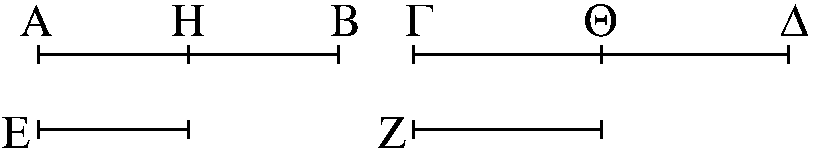
\includegraphics[width=0.8\textwidth]{Book05/fig01g.pdf}}

\gr{Ἐπεὶ γὰρ ἰσάκις ἐστὶ πολλαπλάσιον τὸ ΑΒ τοῦ Ε καὶ τὸ ΓΔ τοῦ
Ζ, ὅσα ἄρα ἐστὶν ἐν τῷ ΑΒ μεγέθη ἴσα τῷ Ε, τοσαῦτα καὶ
ἐν τῷ ΓΔ ἴσα τῷ Ζ. διῃρήσθω τὸ μὲν ΑΒ εἰξ τὰ τῷ Ε μεγέθη ἴσα τὰ ΑΗ, ΗΒ, τὸ δὲ ΓΔ εἰξ τὰ τῷ Ζ ἴσα τὰ ΓΘ, ΘΔ;
ὸέσται δὴ  ἴσον τὸ πλῆθος τῶν ΑΗ, ΗΒ τῷ πλήθει
τῶν ΓΘ, ΘΔ. καὶ ἐπεὶ  ἴσον ἐστὶ τὸ μὲν ΑΗ τῷ Ε, τὸ δὲ 
ΓΘ τῷ Ζ,  ἴσον ἄρα τὸ ΑΗ τῷ Ε, καὶ τὰ ΑΗ, ΓΘ τοῖς Ε, Ζ. διὰ
τὰ αὐτὰ δὴ  ἴσον ἐστὶ τὸ ΗΒ τῷ Ε, καὶ τὰ ΗΒ, ΘΔ τοῖς
Ε, Ζ; ὅσα ἄρα ἐστὶν ἐν τῷ ΑΒ ἴσα τῷ Ε, τοσαῦτα καὶ ἐν τοῖς
ΑΒ, ΓΔ ἴσα τοῖς Ε, Ζ; ὁσαπλάσιον ἄρα ἐστὶ τὸ ΑΒ τοῦ Ε,
τοσαυταπλάσιαὸέσται καὶ τὰ ΑΒ, ΓΔ τῶν Ε, Ζ.}

\gr{Ἐὰν ἄραὸῆ| ὁποσαοῦν μεγέθη ὁποσωνοῦν μεγεθῶνὸίσων τὸ πλῆθος
ὁέκαστον ἑκάστου ἰσάκις πολλαπλάσιον, ὁσαπλάσιόν ἐστιν ὁὲν
τῶν μεγεθῶν ἑνόξ, τοσαυταπλάσιαὸέσται καὶ τὰ πάντα τῶν πάντων;
ὅπερ ἔδει δεῖχαι.}}

\ParallelRText{
\begin{center}
{\large Proposition 1}$^\dag$
\end{center}

If there are any number of magnitudes whatsoever (which are)  equal multiples, respectively, of
some (other) magnitudes,  of equal number (to them), (then) as many times as one of the (first) magnitudes is (divisible) by one (of the second), so many times
will all (of the first magnitudes) also (be divisible) by all (of the second).

Let there be any number of magnitudes whatsoever, $AB$, $CD$, (which are) equal multiples,
respectively, of some (other) magnitudes, $E$, $F$,  of equal  number
(to them). I say that as many times as $AB$ is (divisible) by $E$, so many times will
$AB$, $CD$ also be (divisible) by $E$, $F$.

% Removed epsf size command
\centerline{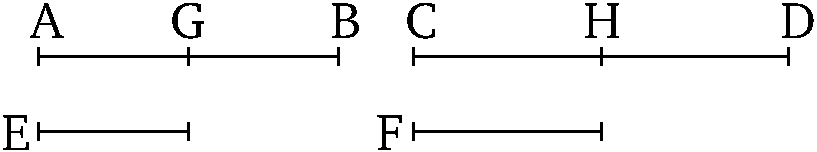
\includegraphics[width=0.8\textwidth]{Book05/fig01e.pdf}}

For since $AB$, $CD$ are equal multiples of $E$, $F$, thus as many
magnitudes as (there) are in  $AB$ equal to $E$, so many (are there) also in $CD$ equal to $F$. Let $AB$ be divided into magnitudes $AG$, $GB$, equal to $E$,
and $CD$ into (magnitudes) $CH$, $HD$, equal to $F$. So, the number of (divisions)
$AG$, $GB$ will be equal to the number of (divisions) $CH$, $HD$. And since
$AG$ is equal to $E$, and $CH$ to $F$,   $AG$ (is)  thus equal to $E$, and $AG$, $CH$ to
$E$, $F$. So, for the same (reasons), $GB$ is equal to $E$, and $GB$, $HD$ to $E$, $F$.
Thus, as many (magnitudes) as (there) are in $AB$ equal to $E$, so many (are there)
also in $AB$, $CD$ equal to $E$, $F$. Thus, as many times as $AB$ is (divisible) by $E$, so many
times will $AB$, $CD$ also be (divisible)  by $E$, $F$.

Thus, if there are any number of magnitudes whatsoever (which are) equal multiples, respectively, of
some (other) magnitudes,  of  equal  number (to them), (then) as many times as one of the (first) magnitudes is (divisible) by one (of the second), so many times
will all (of the first magnitudes) also (be divisible) by all (of the second). (Which is)
the very thing it was required to show.}
\end{Parallel}
{\footnotesize \noindent$^\dag$ In modern notation, this proposition
reads $m\,\alpha + m\,\beta +\cdots= m\,(\alpha+\beta+\cdots)$.}

%%%%%%
% Prop 5.2
%%%%%%
\pdfbookmark[1]{Proposition 5.2}{pdf5.2}
\begin{Parallel}{}{} 
\ParallelLText{
\begin{center}
{\large \ggn{2}.}
\end{center}\vspace*{-7pt}

\gr{Ἐὰν πρῶτον δευτέρου ἰσάκιςὸῆ| πολλαπλάσιον καὶ τρίτον τετάρτου, ὸῆ|
δὲ καὶ πέμπτον δευτέρου ἰσάκις πολλαπλάσιον καὶ ὁέκτον τετάρτου, καὶ
συντεθὲν πρῶτον καὶ πέμπτον δευτέρου ἰσάκιςὸέσται πολλαπλάσιον
καὶ τρίτον καὶ ὁέκτον τετάρτου.}

\gr{Πρῶτον γὰρ τὸ ΑΒ δευτέρου τοῦ Γ ἰσάκιςὸέστω πολλαπλάσιον καὶ
τρίτον τὸ ΔΕ τετάρτου τοῦ Ζ, ὸέστω δὲ καὶ πέμπτον τὸ ΒΗ δευτέρου τοῦ
Γ ἰσάκις πολλαπλάσιον καὶ ὁέκτον τὸ ΕΘ τετάρτου τοῦ Ζ; λέγω,
ὅτι καὶ συντεθὲν πρῶτον καὶ πέμπτον τὸ ΑΗ δευτέρου τοῦ 
Γ ἰσάκιςὸέσται πολλαπλάσιον καὶ τρίτον καὶ ὁέκτον
τὸ ΔΘ τετάρτου τοῦ Ζ.}

\gr{Ἐπεὶ γὰρ ἰσάκις ἐστὶ πολλαπλάσιον τὸ ΑΒ τοῦ Γ καὶ τὸ 
ΔΕ τοῦ Ζ, ὅσα ἄρα ἐστὶν ἐν τῷ ΑΒ ἴσα τῷ Γ, τοσαῦτα καὶ ἐν
τῷ ΔΕ ἴσα τῷ Ζ. διὰ τὰ αὐτὰ δὴ καὶ ὅσα ἐστὶν ἐν τῷ ΒΗ ἴσα τῷ Γ, τοσαῦτα καὶ ἐν τῷ ΕΘ ἴσα τῷ Ζ; ὅσα ἄρα ἐστὶν
ἐν ὅλῳ τῷ ΑΗ ἴσα τῷ Γ, τοσαῦτα καὶ ἐν ὅλῳ τῷ ΔΘ ἴσα τῷ
Ζ; ὁσαπλάσιον ἄρα ἐστὶ τὸ ΑΗ τοῦ Γ, τοσαυταπλάσιονὸέσται καὶ τὸ
ΔΘ τοῦ Ζ. καὶ συντεθὲν ἄρα πρῶτον καὶ πέμπτον τὸ ΑΗ δευτέρου
τοῦ Γ ἰσάκιςὸέσται πολλαπλάσιον καὶ τρίτον καὶ ὁέκτον τὸ
ΔΘ τετάρτου τοῦ Ζ.}\\~\\~\\~\\~\\~\\~\\~\\~\\

% Removed epsf size command
\centerline{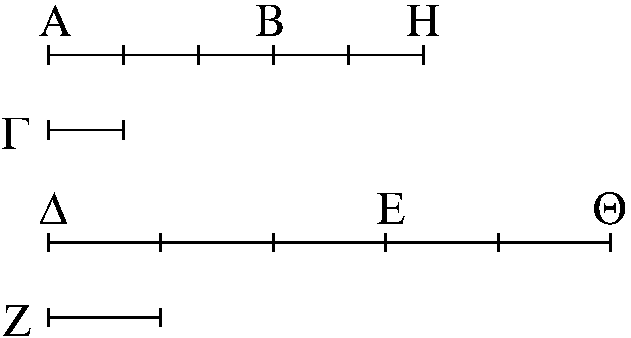
\includegraphics[width=0.8\textwidth]{Book05/fig02g.pdf}}

\gr{Ἐὰν ἄρα πρῶτον δευτέρου ἰσάκιςὸῆ| πολλαπλάσιον καὶ τρίτον τετάρτου, ὸῆ|
δὲ καὶ πέμπτον δευτέρου ἰσάκις πολλαπλάσιον καὶ ὁέκτον τετάρτου, καὶ
συντεθὲν πρῶτον καὶ πέμπτον δευτέρου ἰσάκιςὸέσται πολλαπλάσιον
καὶ τρίτον καὶ ὁέκτον τετάρτου; ὅπερ ἔδει δεῖχαι.}}

\ParallelRText{
\begin{center}
{\large Proposition 2}$^{\dag}$
\end{center}

If a first (magnitude) and a third are equal multiples of a second
and a fourth (respectively), and a fifth (magnitude) and a sixth (are) also equal multiples of the
second and fourth (respectively), (then) the first (magnitude) and the fifth, being added together, and the third and the sixth,  (being added together), will also be equal multiples of the
second (magnitude) and the fourth (respectively).

For let a first (magnitude) $AB$ and a third $DE$ be equal multiples of a
second $C$ and a fourth $F$ (respectively). And let a fifth (magnitude) $BG$
and a sixth $EH$ also be (other) equal multiples of the second $C$ and the fourth $F$
(respectively). I say that the first (magnitude) and the fifth, being added together, (to give) $AG$,
and the third (magnitude) and the sixth, (being added together, to give) $DH$, will also be
equal multiples of the second (magnitude) $C$ and the fourth $F$ (respectively).

For since $AB$ and $DE$ are equal multiples of $C$ and $F$ (respectively), 
thus as many (magnitudes) as (there) are in $AB$ equal to $C$, so many (are there) also
in $DE$ equal to $F$.  And so, for the same (reasons),   as many (magnitudes) as (there) are in $BG$ equal to $C$, so many (are there) also in $EH$ equal to $F$.
Thus, as many (magnitudes) as (there) are in the whole of $AG$ equal to $C$,
so many (are there) also in the whole of $DH$ equal to $F$.
Thus, as many times as $AG$ is (divisible) by $C$, so many times will $DH$ also
be divisible by $F$. Thus, the first (magnitude) and the fifth, being
added together, (to give) $AG$, and the third (magnitude) and the sixth, (being
added together, to give) $DH$, will also be equal multiples of the second (magnitude)
$C$ and the fourth $F$ (respectively).

% Removed epsf size command
\centerline{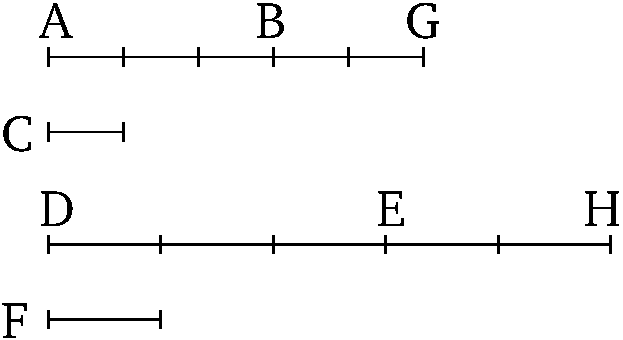
\includegraphics[width=0.8\textwidth]{Book05/fig02e.pdf}}

Thus, if a first (magnitude) and a third are equal multiples of a second
and a fourth (respectively), and a fifth (magnitude) and a sixth (are) also equal multiples of the
second and fourth (respectively), (then) the  first (magnitude) and the fifth, being
added together, and the third  and sixth, (being added together), will also be equal multiples of the
second (magnitude) and the fourth (respectively). (Which is) the very thing it was required to
show.}
\end{Parallel}
{\footnotesize \noindent$^\dag$ In modern notation, this propostion reads
$m\,\alpha+n\,\alpha = (m+n)\,\alpha$.}

%%%%%%
% Prop 5.3
%%%%%%
\pdfbookmark[1]{Proposition 5.3}{pdf5.3}
\begin{Parallel}{}{} 
\ParallelLText{
\begin{center}
{\large \ggn{3}.}
\end{center}\vspace*{-7pt}

\gr{Ἐὰν πρῶτον δευτέρου ἰσάκιςὸῆ| πολλαπλάσιον καὶ τρίτον τετάρτου,
ληφθῆ| δὲ ἰσάκις πολλαπλάσια τοῦ τε πρώτου καὶ τρίτου, καὶ διὸ 
ὸίσου τῶν  ληφθέντων ἑκάτερον ἑκατέρου ἰσάκιςὸέσται πολλαπλάσιον
τὸ μὲν τοῦ δευτέρου τὸ δὲ τοῦ τετάρτου.}

\gr{Πρῶτον γὰρ τὸ Α δευτέρου τοῦ Β ἰσάκιςὸέστω πολλαπλάσιον καὶ
τρίτον τὸ Γ τετάρτου τοῦ Δ, καὶ εἰλήφθω τῶν Α, Γ ἰσάκις πολλαπλάσια
τὰ ΕΖ, ΗΘ; λέγω, ὅτι ἰσάκις ἐστὶ πολλαπλάσιον τὸ ΕΖ τοῦ Β καὶ
τὸ ΗΘ τοῦ Δ.}

\gr{Ἐπεὶ γὰρ ἰσάκις ἐστὶ πολλαπλάσιον τὸ ΕΖ τοῦ Α καὶ τὸ ΗΘ τοῦ
Γ, ὅσα ἄρα ἐστὶν ἐν τῷ ΕΖ ἴσα τῷ Α, τοσαῦτα καὶ ἐν τῷ
ΗΘ ἴσα τῷ Γ. διῃρήσθω τὸ μὲν ΕΖ εἰξ τὰ τῷ Α μεγέθη ἴσα
τὰ ΕΚ, ΚΖ, τὸ δὲ ΗΘ εἰξ τὰ τῷ Γ ἴσα τὰ ΗΛ, ΛΘ; ὸέσται δὴ  ἴσον
τὸ πλῆθος τῶν ΕΚ, ΚΖ τῷ πλήθει τῶν ΗΛ, ΛΘ. καὶ ἐπεὶ
ἰσάκις ἐστὶ πολλαπλάσιον τὸ Α τοῦ Β καὶ τὸ Γ τοῦ Δ,   ἴσον δὲ τὸ
μὲν ΕΚ τῷ Α, τὸ δὲ ΗΛ τῷ Γ, ἰσάκις ἄρα ἐστὶ πολλαπλάσιον
τὸ ΕΚ τοῦ Β καὶ τὸ ΗΛ τοῦ Δ. διὰ τὰ αὐτὰ δὴ ἰσάκις ἐστὶ
πολλαπλάσιον τὸ ΚΖ τοῦ Β καὶ τὸ ΛΘ τοῦ Δ. ἐπεὶ ο~ὐν
πρῶτον τὸ ΕΚ δευτέρου τοῦ Βὸίσάκις ἐστὶ πολλαπλάσιον καὶ
τρίτον τὸ ΗΛ τετάρτου τοῦ Δ, ὸέστι δὲ καὶ πέμπτον τὸ ΚΖ δευτέρου τοῦ
Β ἰσάκις πολλαπλάσιον καὶ ὁέκτον τὸ ΛΘ τετάρτου τοῦ Δ,
καὶ συντεθὲν ἄρα πρῶτον καὶ πέμπτον τὸ ΕΖ δευτέρου τοῦ Β
ἰσάκις ἐστὶ πολλαπλάσιον καὶ τρίτον καὶ ὁέκτον τὸ ΗΘ
τετάρτου τοῦ Δ.}\\~\\~\\~\\~\\~\\

% Removed epsf size command
\centerline{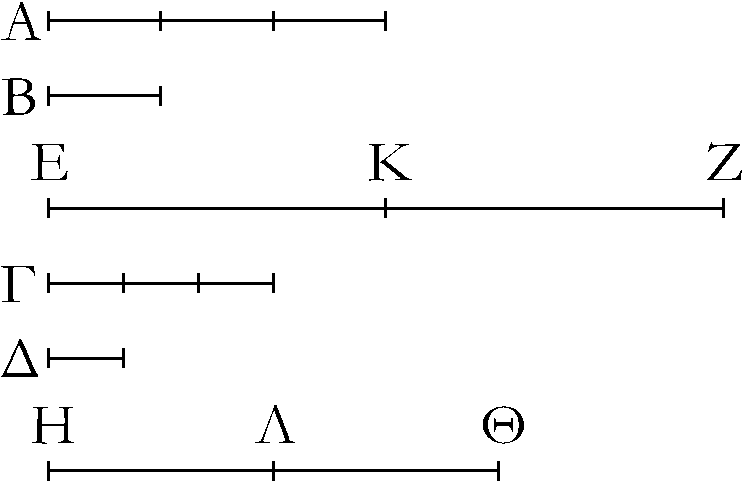
\includegraphics[width=0.8\textwidth]{Book05/fig03g.pdf}}

\gr{Ἐὰν ἄρα πρῶτον δευτέρου ἰσάκιςὸῆ| πολλαπλάσιον καὶ τρίτον τετάρτου,
ληφθῆ| δὲ τοῦ πρώτου καὶ τρίτου ἰσάκις πολλαπλάσια, καὶ διὸ 
ὸίσου τῶν  ληφθέντων ἑκάτερον ἑκατέρου ἰσάκιςὸέσται πολλαπλάσιον
τὸ μὲν τοῦ δευτέρου τὸ δὲ τοῦ τετάρτου; ὅπερ ἔδει δεῖχαι.}}

\ParallelRText{
\begin{center}
{\large Proposition 3}$^\dag$
\end{center}

If a first (magnitude) and a third are equal multiples
of a second and a fourth (respectively), and equal multiples are taken of the
first and the third, (then), via equality,  the 
(magnitudes) taken will also be equal multiples of the second (magnitude) and the fourth, respectively.

For let a first (magnitude) $A$ and a third $C$ be equal multiples of a
second $B$ and a fourth $D$ (respectively), and let the equal multiples
$EF$ and $GH$ be taken of $A$ and $C$ (respectively). I say that
$EF$ and $GH$ are equal multiples of $B$ and $D$ (respectively).

For since $EF$ and $GH$ are equal multiples of $A$ and $C$ (respectively), thus as many (magnitudes) as (there) are in $EF$ equal to $A$, so many (are there) also in
$GH$ equal to $C$. Let $EF$ be divided into magnitudes $EK$, $KF$ equal
to $A$, and $GH$ into (magnitudes) $GL$, $LH$ equal to $C$. So, the number of (magnitudes)
$EK$, $KF$ will be equal to the number of (magnitudes) $GL$, $LH$.
And since $A$ and $C$ are equal multiples of $B$ and $D$ (respectively), and $EK$ (is)
equal to $A$, and $GL$ to $C$,  $EK$ and $GL$ are thus equal multiples of $B$ and $D$
(respectively). So, for the same (reasons), $KF$ and $LH$ are equal multiples
of $B$ and $D$ (respectively). Therefore, since the first (magnitude) $EK$ and the
third $GL$ are equal multiples of the second $B$ and the fourth $D$ (respectively), and the fifth (magnitude) $KF$ and
the sixth $LH$ are  also  equal multiples of the second $B$ and the fourth $D$ (respectively),  then  the first (magnitude) and fifth, being added together,
(to give) $EF$, and the third (magnitude) and sixth, (being added together, to give) $GH$, are thus also equal multiples of the second (magnitude) $B$ and the fourth $D$ (respectively) [Prop.~5.2].

% Removed epsf size command
\centerline{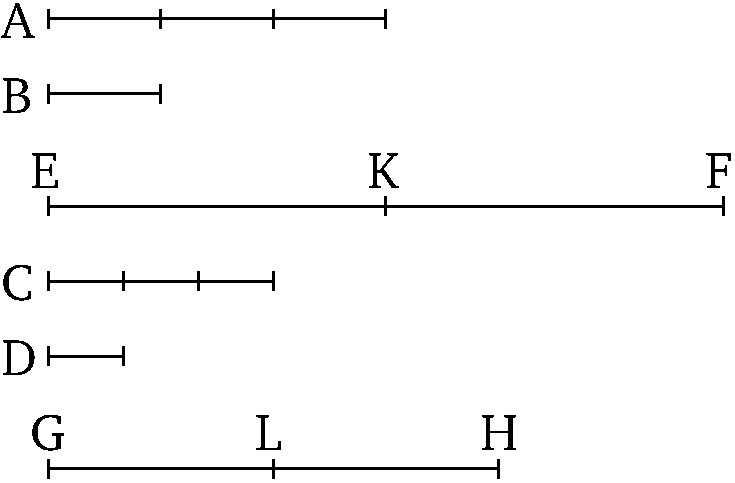
\includegraphics[width=0.8\textwidth]{Book05/fig03e.pdf}}

Thus, if a first (magnitude) and a third are equal multiples
of a second and a fourth (respectively), and equal multiples are taken of the
first and the third, (then), via equality,  the 
(magnitudes) taken will also be equal multiples of the second (magnitude) and the fourth, respectively. (Which is) the very thing it was required to show.}
\end{Parallel}
{\footnotesize \noindent$^\dag$ In modern notation, this proposition reads
$m\,(n\,\alpha) = (m\,n)\,\alpha$.}


%%%%%%
% Prop 5.4
%%%%%%
\pdfbookmark[1]{Proposition 5.4}{pdf5.4}
\begin{Parallel}{}{} 
\ParallelLText{
\begin{center}
{\large \ggn{4}.}
\end{center}\vspace*{-7pt}

\gr{Ἐὰν πρῶτον πρὸς δεύτερον τὸν αὐτὸνὸέθῃ λόγον καὶ τρίτον
πρὸς τέταρτον, καὶ τὰ ἰσάκις πολλαπλάσια τοῦ τε πρώτου καὶ
τρίτου πρὸς τὰ ἰσάκις πολλαπλάσια τοῦ δευτέρου καὶ τετάρτου καθὸ
ὁποιονοῦν πολλαπλασιασμὸν τὸν αὐτὸν ὁέχει λόγον ληφθέντα
κατάλληλα.}

\gr{Πρῶτον γὰρ τὸ Α πρὸς δεύτερον τὸ Β τὸν αὐτὸν ἐθέτω λόγον
καὶ τρίτον τὸ Γ πρὸς τέταρτον τὸ Δ, καὶ εἰλήφθω τῶν μὲν Α, Γ
ἰσάκις πολλαπλάσια τὰ Ε, Ζ, τῶν δὲ Β, Δὸάλλα, ὁὰ ὸέτυθεν, ἰσάκις
πολλαπλάσια τὰ Η, Θ; λέγω, ὅτι ἐστὶν ὡξ τὸ Ε πρὸς τὸ Η, οὁύτως 
τὸ Ζ πρὸς τὸ Θ.}

\gr{Εἰλήφθω γὰρ τῶν μὲν Ε, Ζ ἰσάκις πολλαπλάσια τὰ Κ, Λ, τῶν δὲ Η,
Θὸάλλα, ὁὰ ὸέτυθεν, ἰσάκις πολλαπλάσια τὰ Μ, Ν.}

\gr{ {[}Ka`i] >epe`i >is'akic >est`i pollapl'asion t`o m`en E to~u A, t`o d`e Z to~u
G, ka`i e>'ilhptai t~wn E, Z >'is'akic pollapl'asia t`a K, L, >'is'akic
>'ara >est`i pollapl'asion t`o K to~u A ka`i t`o L to~u G. di`a t`a a\kern -.7pt >ut`a d`h
>is'akic >est`i pollapl'asion t`o M to~u B ka`i t`o N to~u D. ka`i >epe'i
>estin <wc t`o A pr`oc t`o B, o<'utwc t`o G pr`oc t`o D, ka`i e>'ilhptai
t~wn m`en A, G >is'akic pollapl'asia t`a K, L, t~wn d`e B, D >'alla, <`a
>'etuqen, >is'akic pollapl'asia t`a M, N, e>i >'ara <uper'eqei t`o K
to~u M, <uper'eqei ka`i t`o L to~u N, ka`i e>i >'ison, >'ison, ka`i
e>i >'elatton, >'elatton. ka'i >esti t`a m`en K, L t~wn E, Z >is'akic 
pollapl'asia, t`a d`e M, N t~wn H, J >'alla, <`a >'etuqen, >is'akic
pollapl'asia;
 >'estin >'ara <wc t`o E pr`oc t`o H, o<'utwc t`o Z
pr`oc t`o J.}\\~\\~\\~\\

% Removed epsf size command
\centerline{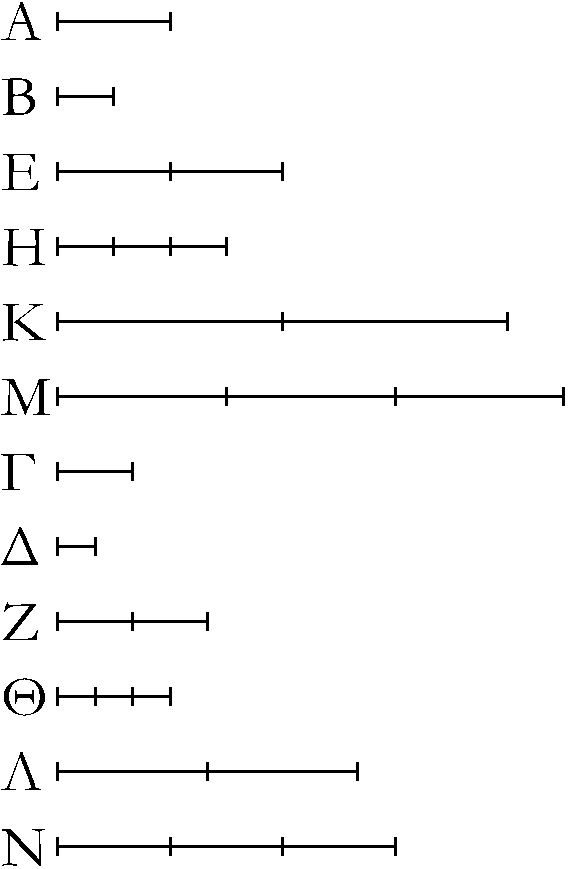
\includegraphics[width=0.8\textwidth]{Book05/fig04g.pdf}}

\gr{Ἐὰν ἄρα πρῶτον πρὸς δεύτερον τὸν αὐτὸνὸέθῃ λόγον καὶ τρίτον
πρὸς τέταρτον, καὶ τὰ ἰσάκις πολλαπλάσια τοῦ τε πρώτου καὶ
τρίτου πρὸς τὰ ἰσάκις πολλαπλάσια τοῦ δευτέρου καὶ τετάρτου τὸν αὐτὸν ὁέχει λόγον καθὸ ὁποιονοῦν πολλαπλασιασμὸν  ληφθέντα
κατάλληλα; ὅπερ ἔδει δεῖχαι.}}

\ParallelRText{
\begin{center}
{\large Proposition 4}$^\dag$
\end{center}

If  a first (magnitude) has the same ratio to a second 
that a third  (has) to a fourth, (then) equal multiples of the first (magnitude) and the third will also have the same ratio to equal multiples of the second and the fourth,  being taken in corresponding order, according to any kind of
multiplication whatsoever.

For let a first (magnitude) $A$ have the same ratio to a second $B$ that
a third $C$  (has) to a fourth $D$. And let equal multiples $E$ and $F$ 
be taken of $A$ and $C$ (respectively), and  other random equal multiples
$G$ and $H$  of $B$ and $D$ (respectively). I say that as $E$ (is)
to $G$, so $F$ (is) to $H$.

For let equal multiples $K$ and $L$ be taken of $E$ and $F$ (respectively),
and other random equal multiples $M$ and $N$ of $G$ and $H$ (respectively).

\mbox{[}And] since $E$ and $F$ are equal multiples of $A$ and $C$ (respectively), and
the equal multiples $K$ and $L$ have been taken of $E$ and $F$ (respectively),
 $K$ and $L$ are thus equal multiples of $A$ and $C$ (respectively) [Prop.~5.3]. So, for the same (reasons), $M$ and $N$
 are equal multiples of $B$ and $D$ (respectively). And since as $A$ is to
 $B$, so $C$ (is) to $D$, and the equal multiples $K$ and $L$ have been taken of $A$ and
 $C$ (respectively), and the other random equal multiples  $M$ and $N$ of $B$ and $D$ (respectively), (then) if $K$ exceeds $M$ (then) $L$ also
 exceeds $N$, and if ($K$ is) equal (to $M$ then $L$ is also) equal (to $N$), and if ($K$ is) less (than $M$ then $L$ is also) less (than $N$) [Def.~5.5]. And $K$ and $L$ are equal multiples of 
 $E$ and $F$ (respectively), and $M$ and $N$ other random equal multiples of $G$ and $H$ (respectively). Thus, as $E$ (is) to $G$, so $F$ (is) to $H$ 
 [Def.~5.5].

% Removed epsf size command
\centerline{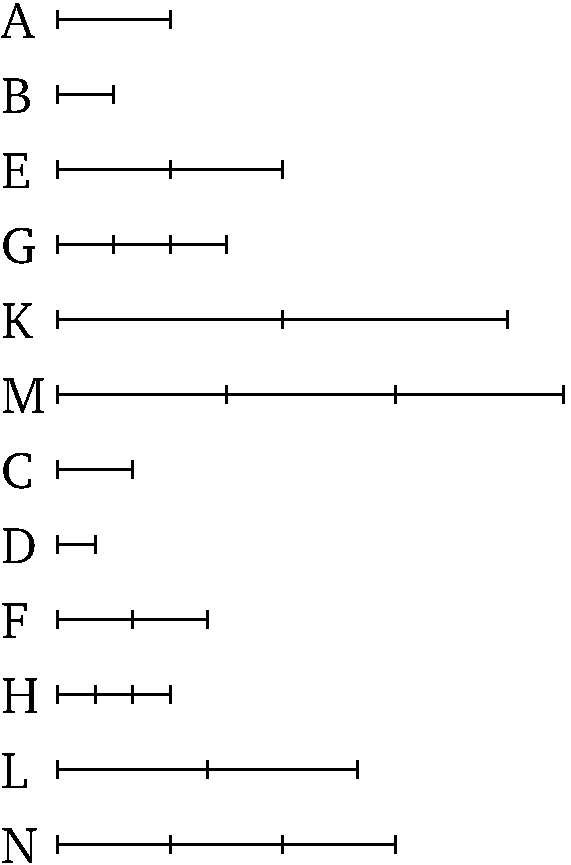
\includegraphics[width=0.8\textwidth]{Book05/fig04e.pdf}}

Thus, if a first (magnitude) has the same ratio to a second 
that a third  (has) to a fourth, (then) equal multiples of the first (magnitude) and the third will also have the same ratio to equal multiples of the second and the fourth,  being taken in corresponding order, according to any kind of
multiplication whatsoever. (Which is) the very thing
it was required to show.}
\end{Parallel}
{\footnotesize \noindent$^\dag$ In modern notation, this
proposition reads that if $\alpha:\beta :: \gamma:\delta$ then
$m\,\alpha:n\,\beta::m\,\gamma:n\,\delta$, for all $m$ and $n$.}

%%%%%%
% Prop 5.5
%%%%%%
\pdfbookmark[1]{Proposition 5.5}{pdf5.5}
\begin{Parallel}{}{} 
\ParallelLText{
\begin{center}
{\large \ggn{5}.}
\end{center}\vspace*{-7pt}

\gr{Ἐὰν μέγεθος μεγέθους ἰσάκιςὸῆ| πολλαπλάσιον, ὅπερ ἀφαιρεθὲν
ἀφαιρεθέντος, καὶ τὸ λοιπὸν τοῦ λοιποῦ ἰσάκιςὸέσται πολλαπλάσιον,
ὁσαπλάσιόν ἐστι τὸ ὅλον τοῦ ὅλου.}\\~\\

% Removed epsf size command
\centerline{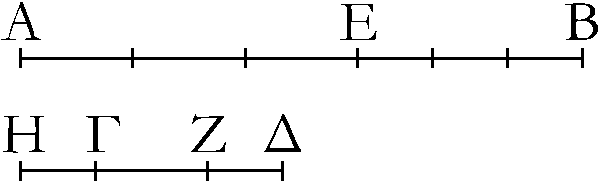
\includegraphics[width=0.8\textwidth]{Book05/fig05g.pdf}}

\gr{Μέγεθος γὰρ τὸ ΑΒ μεγέθους τοῦ ΓΔ ἰσάκιςὸέστω πολλαπλάσιον,
ὅπερ ἀφαιρεθὲν τὸ ΑΕ ἀφαιρεθέντος τοῦ ΓΖ; λέγω, ὅτι καὶ λοιπὸν
τὸ ΕΒ λοιποῦ τοῦ ΖΔ ἰσάκιςὸέσται πολλαπλάσιον, ὁσαπλάσιόν 
ἐστιν ὅλον τὸ ΑΒ ὅλου τοῦ ΓΔ.}

\gr{Ὁσαπλάσιον γάρ ἐστι τὸ ΑΕ τοῦ ΓΖ, τοσαυταπλάσιον γεγονέτω καὶ
τὸ ΕΒ τοῦ ΓΗ.}

\gr{Καὶ ἐπεὶ ἰσάκις ἐστὶ πολλαπλάσιον τὸ ΑΕ τοῦ ΓΖ καὶ τὸ ΕΒ τοῦ
ΗΓ, ἰσάκις ἄρα ἐστὶ πολλαπλάσιον τὸ ΑΕ τοῦ ΓΖ καὶ τὸ ΑΒ τοῦ
ΗΖ. κεῖται δὲ ἰσάκις πολλαπλάσιον τὸ ΑΕ τοῦ ΓΖ καὶ τὸ ΑΒ τοῦ
ΓΔ. ἰσάκις ἄρα ἐστὶ πολλαπλάσιον τὸ ΑΒ ἑκατέρου τῶν ΗΖ, ΓΔ;
 ἴσον ἄρα τὸ ΗΖ τῷ ΓΔ. κοινὸν ἀφῃρήσθω τὸ ΓΖ; λοιπὸν ἄρα τὸ ΗΓ λοιπῶ| τῷ ΖΔ ἴσον ἐστίν. καὶ ἐπεὶ ἰσάκις
ἐστὶ πολλαπλάσιον τὸ ΑΕ τοῦ ΓΖ καὶ τὸ ΕΒ τοῦ ΗΓ,  ἴσον
δὲ τὸ ΗΓ τῷ  ΔΖ, 
ἰσάκις ἄρα  ἐστὶ πολλαπλάσιον τὸ ΑΕ τοῦ ΓΖ καὶ τὸ ΕΒ τοῦ ΖΔ.
ἰσάκις δὲ ὑπόκειται πολλαπλάσιον τὸ ΑΕ τοῦ ΓΖ καὶ τὸ ΑΒ τοῦ
ΓΔ; ἰσάκις ἄρα 
ἐστὶ πολλαπλάσιον τὸ ΕΒ τοῦ ΖΔ καὶ τὸ ΑΒ τοῦ ΓΔ. καὶ λοιπὸν ἄρα τὸ ΕΒ λοιποῦ τοῦ ΖΔ ἰσάκιςὸέσται πολλαπλάσιον, ὁσαπλάσιόν
ἐστιν ὅλον τὸ ΑΒ ὅλου τοῦ ΓΔ.}

\gr{Ἐὰν ἄρα μέγεθος μεγέθους ἰσάκιςὸῆ| πολλαπλάσιον, ὅπερ ἀφαιρεθὲν
ἀφαιρεθέντος, καὶ τὸ λοιπὸν τοῦ λοιποῦ ἰσάκιςὸέσται πολλαπλάσιον,
ὁσαπλάσιόν ἐστι καὶ τὸ ὅλον τοῦ ὅλου; ὅπερ ἔδει δεῖχαι.}}

\ParallelRText{
\begin{center}
{\large Proposition 5}$^\dag$
\end{center}

If a magnitude is the same multiple of a magnitude
that a (part) taken away (is) of a (part) taken away (respectively), (then) the remainder will
also be the same multiple of the remainder as that  which the whole (is) of the whole (respectively).

% Removed epsf size command
\centerline{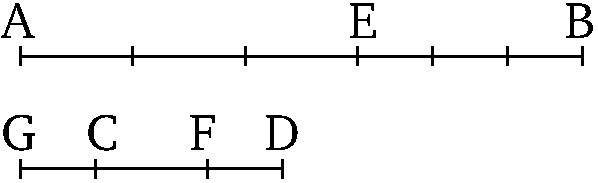
\includegraphics[width=0.8\textwidth]{Book05/fig05e.pdf}}

For let the magnitude $AB$ be the same multiple of the magnitude $CD$ that
the (part)  taken away $AE$ (is) of the (part)  taken away $CF$ (respectively).
I say that the remainder $EB$ will also be the same multiple
of the remainder $FD$ as that which the whole $AB$ (is) of the whole
$CD$ (respectively).

For as many times as $AE$ is (divisible) by $CF$, so many times let $EB$
also be made (divisible) by $CG$.

And since $AE$ and $EB$ are equal multiples of $CF$ and $GC$ (respectively),
$AE$ and $AB$ are thus equal multiples of $CF$ and $GF$ (respectively) 
 [Prop.~5.1]. And  $AE$ and $AB$ are assumed (to be) equal multiples of $CF$ and $CD$ (respectively). Thus,
 $AB$ is an equal multiple of each of $GF$ and $CD$. Thus, $GF$ (is) equal to
 $CD$. Let $CF$ be subtracted from both. Thus, the remainder $GC$ is
 equal to the remainder $FD$. And since $AE$ and $EB$ are equal multiples
 of $CF$ and $GC$ (respectively), and $GC$ (is) equal to $DF$, $AE$  and $EB$ are thus
 equal multiples of $CF$ and $FD$ (respectively). And $AE$ and $AB$ are assumed
 (to be) equal multiples of $CF$ and $CD$ (respectively). Thus, $EB$ and $AB$ are
 equal multiples of $FD$ and $CD$ (respectively). Thus, the remainder
 $EB$ will also be the same multiple of the remainder $FD$
 as that which the whole $AB$ (is) of the whole $CD$ (respectively).
 
 Thus, if a magnitude is the same multiple of a magnitude
that a (part) taken away (is) of a (part) taken away (respectively), (then) the remainder will
also be the same multiple of the remainder as that  which the whole (is) of the whole (respectively).
  (Which is) the very thing it was required to show.}
\end{Parallel}
{\footnotesize \noindent$^\dag$ In modern notation, this
proposition reads $m\,\alpha-m\,\beta=m\,(\alpha-\beta)$.}

%%%%%%
% Prop 5.6
%%%%%%
\pdfbookmark[1]{Proposition 5.6}{pdf5.6}
\begin{Parallel}{}{} 
\ParallelLText{
\begin{center}
{\large \ggn{6}.}
\end{center}\vspace*{-7pt}

\gr{Ἐὰν δύο μεγέθη δύο μεγεθῶν ἰσάκιςὸῆ| πολλαπλάσια, καὶ ἀφαιρεθέντα
τινὰ τῶν αὐτῶν ἰσάκιςὸῆ| πολλαπλάσια, καὶ τὰ λοιπὰ τοῖς αὐτοῖς ἢτοι ἴσα ἐστὶνὸὴ ἰσάκις αὐτῶν πολλαπλάσια.}

\gr{Δύο γὰρ μεγέθη τὰ ΑΒ, ΓΔ δύο μεγεθῶν τῶν Ε, Ζ ἰσάκιςὸέστω
πολλαπλάσια, καὶ ἀφαιρεθέντα τὰ ΑΗ, ΓΘ τῶν αὐτῶν τῶν Ε, Ζ ἰσάκιςὸέστω πολλαπλάσια;  λέγω, ὅτι καὶ λοιπὰ τὰ ΗΒ, ΘΔ τοῖς Ε, Ζ ἢτοι ἴσα ἐστὶνὸὴ ἰσάκις αὐτῶν πολλαπλάσια.}\\~\\~\\

% Removed epsf size command
\centerline{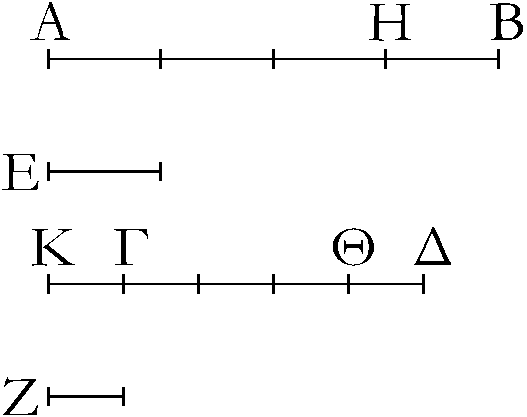
\includegraphics[width=0.8\textwidth]{Book05/fig06g.pdf}}

\gr{Ἔστω γὰρ πρότερον τὸ ΗΒ τῷ Ε ἴσον; λέγω, ὅτι καὶ τὸ ΘΔ τῷ Ζ ἴσον ἐστίν.}

\gr{Κείσθω γὰρ τῷ Ζ ἴσον τὸ ΓΚ. ἐπεὶ ἰσάκις ἐστὶ πολλαπλάσιον
τὸ ΑΗ τοῦ Ε καὶ τὸ ΓΘ τοῦ Ζ,   ἴσον δὲ τὸ μὲν ΗΒ τῷ Ε,
τὸ δὲ ΚΓ τῷ Ζ, ἰσάκις ἄρα ἐστὶ πολλαπλάσιον τὸ ΑΒ τοῦ Ε καὶ
τὸ ΚΘ τοῦ Ζ. ἰσάκις δὲ ὑπόκειται πολλαπλάσιον τὸ ΑΒ τοῦ Ε καὶ
τὸ ΓΔ τοῦ Ζ; ὸίσάκις ἄρα ἐστὶ πολλαπλάσιον τὸ ΚΘ τοῦ Ζ καὶ τὸ ΓΔ τοῦ Ζ. ἐπεὶ οὸῦν ἑκάτερον τῶν ΚΘ, ΓΔ
τοῦ Ζ ἰσάκις ἐστὶ πολλαπλάσιον,  ἴσον ἄρα ἐστὶ τὸ ΚΘ τῷ ΓΔ.
κοινὸν ἀφῃρήσθω τὸ ΓΘ; λοιπὸν ἄρα τὸ ΚΓ λοιπῶ| τῷ ΘΔ ἴσον ἐστίν. ἀλλὰ τὸ Ζ τῷ ΚΓ ἐστιν ἴσον; καὶ τὸ ΘΔ ἄρα
τῷ Ζ ἴσον ἐστίν. ὁώστε εἰ τὸ ΗΒ τῷ Ε ἴσον ἐστίν, καὶ τὸ ΘΔ ἴσονὸέσται τῷ Ζ.}

\gr{Ὁμοίως δὴ δείχομεν, ὅτι, κὸὰ|ν πολλαπλάσιονὸῆ| τὸ ΗΒ τοῦ Ε,
τοσαυταπλάσιονὸέσται καὶ τὸ ΘΔ τοῦ Ζ.}

\gr{Ἐὰν ἄρα δύο μεγέθη δύο μεγεθῶν ἰσάκιςὸῆ| πολλαπλάσια, καὶ ἀφαιρεθέντα
τινὰ τῶν αὐτῶν ἰσάκιςὸῆ| πολλαπλάσια, καὶ τὰ λοιπὰ τοῖς αὐτοῖς ἢτοι ἴσα ἐστὶνὸὴ ἰσάκις αὐτῶν πολλαπλάσια; ὅπερ ἔδει
δεῖχαι.}}

\ParallelRText{
\begin{center}
{\large Proposition 6}$^\dag$
\end{center}

If two magnitudes are equal multiples of two (other) magnitudes, and some (parts) taken away (from the former magnitudes) are equal multiples of the latter (magnitudes, respectively),
(then) the remainders  are also either equal to the latter (magnitudes), or (are) equal multiples of them (respectively).

For let two magnitudes $AB$ and $CD$ be equal multiples of two magnitudes
$E$ and $F$ (respectively). And let the (parts)  taken away (from the former) $AG$ and $CH$ be equal multiples of $E$ and $F$ (respectively). I say that the remainders $GB$ and
$HD$ are also either equal to $E$ and $F$ (respectively), or (are) equal multiples of them.

% Removed epsf size command
\centerline{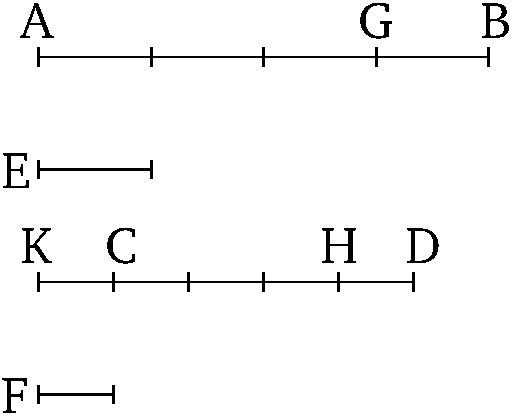
\includegraphics[width=0.8\textwidth]{Book05/fig06e.pdf}}

For let $GB$ be, first of all, equal to $E$. I say that $HD$ is also equal to $F$.

For let  $CK$ be made equal to $F$. Since $AG$ and $CH$ are equal multiples of $E$ and $F$ (respectively), and $GB$ (is) equal to $E$, and $KC$ to $F$,
$AB$ and $KH$ are thus equal multiples of $E$ and $F$ (respectively)
[Prop.~5.2].
And $AB$ and $CD$ are assumed (to be) equal multiples of $E$ and $F$ (respectively). Thus, $KH$ and $CD$ are equal multiples of $F$ and $F$ (respectively). Therefore, $KH$ and $CD$ are each equal multiples of $F$. Thus, $KH$
is equal to $CD$. Let $CH$  be taken away from both. Thus, the remainder
$KC$ is equal to the remainder $HD$. But, $F$ is equal to $KC$. Thus, $HD$ is also equal to $F$. Hence, if $GB$ is equal to $E$, (then) $HD$ will also be equal to $F$.

So, similarly, we can show that even if $GB$ is a multiple of $E$, (then) $HD$
will also be the same multiple of $F$.

Thus, if two magnitudes are equal multiples of two (other) magnitudes, and some (parts) taken away (from the former magnitudes) are equal multiples of the latter (magnitudes, respectively),
(then) the remainders  are also either equal to the latter (magnitudes), or (are) equal multiples of them (respectively). (Which is) the very thing it was required to show.}
\end{Parallel}
{\footnotesize \noindent$^\dag$ In modern notation, this
proposition reads $m\,\alpha-n\,\alpha = (m-n)\,\alpha$.}

%%%%%%
% Prop 5.7
%%%%%%
\pdfbookmark[1]{Proposition 5.7}{pdf5.7}
\begin{Parallel}{}{} 
\ParallelLText{
\begin{center}
{\large \ggn{7}.}
\end{center}\vspace*{-7pt}

\gr{Τὰ  ἴσα πρὸς τὸ αὐτὸ τὸν αὐτὸν ἔχει λόγον καὶ τὸ αὐτὸ πρὸς
τὰ  ἴσα.}

\gr{Ἔστω ἴσα μεγέθη τὰ Α, Β, ὸάλλο δέ τι, ὃ ὸέτυθεν,
μέγεθος τὸ Γ; λέγω, ὅτι ἑκάτερον τῶν Α, Β πρὸς τὸ Γ τὸν
αὐτὸν ἔχει λόγον, καὶ τὸ Γ πρὸς ἑκάτερον τῶν Α, Β.}\\

% Removed epsf size command
\centerline{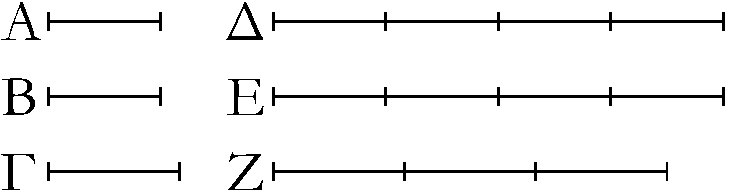
\includegraphics[width=0.8\textwidth]{Book05/fig07g.pdf}}

\gr{Εἰλήφθω γὰρ τῶν μὲν Α, Β ἰσάκις πολλαπλάσια τὰ Δ, Ε, τοῦ δὲ Γὸάλλο, ὃ ὸέτυθεν, πολλαπλάσιον τὸ Ζ.}

\gr{Ἐπεὶ οὸῦν ἰσάκις ἐστὶ πολλαπλάσιον τὸ Δ τοῦ Α καὶ τὸ Ε τοῦ Β,
 ἴσον δὲ τὸ Α τῷ Β,  ἴσον ἄρα καὶ τὸ Δ τῷ Ε. ὸάλλο δέ, ὅ ὸέτυθεν,
τὸ Ζ. εἰ  ἄρα ὑπερέθει τὸ Δ τοῦ Ζ, ὑπερέθει καὶ τὸ Ε τοῦ Ζ, καὶ
εἰ  ἴσον,  ἴσον, καὶ εἰ ὸέλαττον, ὸέλαττον. καί ἐστι τὰ μὲν Δ, Ε
τῶν Α, Β ἰσάκις πολλαπλάσια, τὸ δὲ Ζ τοῦ Γὸάλλο, ὃ ὸέτυθεν,
πολλαπλάσιον; ὸέστιν ἄρα ὡξ τὸ Α πρὸς τὸ Γ, οὁύτως τὸ Β πρὸς τὸ
Γ.}

\gr{Λέγω [δή], ὅτι καὶ τὸ Ε πρὸς ἑκάτερον τῶν Α, Β τὸν αὐτὸν ἔχει λόγον.}

\gr{Τῶν γὰρ αὐτῶν κατασκευασθέντων ὁμοίως δείχομεν, ὅτι ἴσον ἐστὶ τὸ Δ τῷ Ε; ὸάλλο δέ τι τὸ Ζ;
εἰ  ἄρα ὑπερέθει τὸ Ζ τοῦ Δ, ὑπερέθει καὶ τοῦ Ε, καὶ εἰ  ἴσον,
 ἴσον, καὶ εἰ ὸέλαττον, ὸέλαττον. καί ἐστι τὸ μὲν Ζ τοῦ Γ
πολλαπλάσιον, τὰ δὲ Δ, Ε τῶν Α, Βὸάλλα, ὁὰ ὸέτυθεν, ἰσάκις
πολλαπλάσια; ὸέστιν ἄρα ὡξ τὸ Γ πρὸς τὸ Α, οὁύτως τὸ Γ πρὸς
τὸ Β.}

\gr{Τὰ  ἴσα ἄρα πρὸς τὸ αὐτὸ τὸν αὐτὸν ἔχει λόγον καὶ τὸ αὐτὸ πρὸς
τὰ  ἴσα.}\\~\\~\\~\\

\begin{center}
{\large \gr{Πόρισμα}.}
\end{center}\vspace*{-7pt}

\gr{Ἐκ δὴ τούτου φανερόν, ὅτι ἒαν μεγέθη τινὰ ἀνάλογονὸῆ|, καὶ
ἀνάπαλιν ἀνάλογονὸέσται. ὅπερ ἔδει δεῖχαι.}}

\ParallelRText{
\begin{center}
{\large Proposition 7}
\end{center}

Equal (magnitudes) have the same ratio to the same 
(magnitude), and the latter (magnitude has the same ratio) to the equal
(magnitudes).

Let $A$ and $B$ be equal magnitudes, and $C$ some other random magnitude.
I say that $A$ and $B$ each have the same ratio to $C$, and (that) $C$ (has the same
ratio) to each of $A$ and $B$.

% Removed epsf size command
\centerline{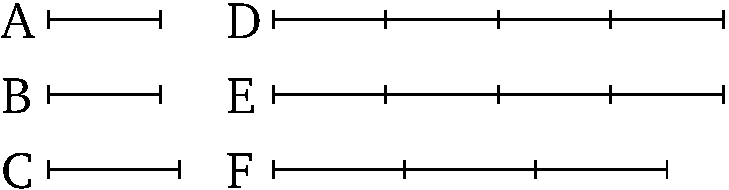
\includegraphics[width=0.8\textwidth]{Book05/fig07e.pdf}}

For let the equal multiples $D$ and $E$ be taken of $A$ and $B$ (respectively), and the other
random multiple $F$ of $C$.

Therefore, since $D$ and $E$ are equal multiples of $A$ and $B$ (respectively), and
$A$ (is) equal to $B$, $D$ (is) thus also equal to $E$. And $F$ (is) different, at random.
Thus, if $D$ exceeds $F$ (then) $E$ also exceeds $F$, and if ($D$ is) equal (to $F$ then
$E$ is also) equal (to $F$), and if ($D$ is) less (than $F$ then
$E$ is also) less (than $F$). And $D$ and $E$ are equal multiples of $A$ and $B$ (respectively), and $F$ another random multiple of $C$. Thus, as $A$ (is) to
$C$, so $B$ (is) to $C$ [Def.~5.5].

\mbox{[}So] I say that $C$$^\dag$ also has the same ratio to each of $A$ and $B$.

For, similarly,  we can show, by the same construction, that $D$ is equal to $E$.
And $F$ (has) some other (value). Thus, if $F$ exceeds $D$ then it also exceeds $E$,
and if ($F$ is) equal (to $D$  then it is also) equal (to $E$), and if ($F$ is) less (than $D$ then it is also) less (than $E$). And $F$ is a multiple of $C$, and $D$ and $E$ other random equal
multiples of $A$ and $B$. Thus, as $C$ (is) to $A$, so $C$ (is)
to $B$  [Def.~5.5]. 

Thus, equal (magnitudes) have the same ratio to the same 
(magnitude), and the latter (magnitude has the same ratio) to the equal
(magnitudes).\\

\begin{center}
\large{Corollary}$^\ddag$
\end{center}\vspace*{-7pt}

So (it is) clear, from this, that if some magnitudes are proportional,
(then) they will also be proportional inversely. (Which is) the very thing it was
required to show.} 
\end{Parallel}
{\footnotesize \noindent$^\dag$ The Greek text has ``$E$'', which is obviously a mistake.\\[0.5ex]
$^\ddag$ In modern notation, this corollary reads that if $\alpha:\beta::\gamma:\delta$ then
$\beta:\alpha::\delta:\gamma$.}

%%%%%%
% Prop 5.8
%%%%%%
\pdfbookmark[1]{Proposition 5.8}{pdf5.8}
\begin{Parallel}{}{} 
\ParallelLText{
\begin{center}
{\large \ggn{8}.}
\end{center}\vspace*{-7pt}

\gr{Τῶν ἀνίσων μεγεθῶν τὸ μεῖζον πρὸς τὸ αὐτὸ μείζονα λόγον ἔχει ἢπερ τὸ ὸέλαττον. καὶ τὸ αὐτὸ πρὸς τὸ ὸέλαττον μείζονα
λόγον ἔχει ἢπερ πρὸς τὸ μεῖζον.}

\gr{Ἔστωὸάνισα μεγέθη τὰ ΑΒ, Γ, καὶ ὸέστω μεῖζον τὸ ΑΒ, ὸάλλο δέ,
ὃ ὸέτυθεν, τὸ Δ; λέγω, ὅτι τὸ ΑΒ πρὸς τὸ Δ μείζονα λόγον ἔχει ἢπερ τὸ Γ πρὸς τὸ Δ, καὶ τὸ Δ πρὸς τὸ Γ μείζονα λόγον ἔχει ἢπερ πρὸς τὸ ΑΒ.}\\

% Removed epsf size command
\centerline{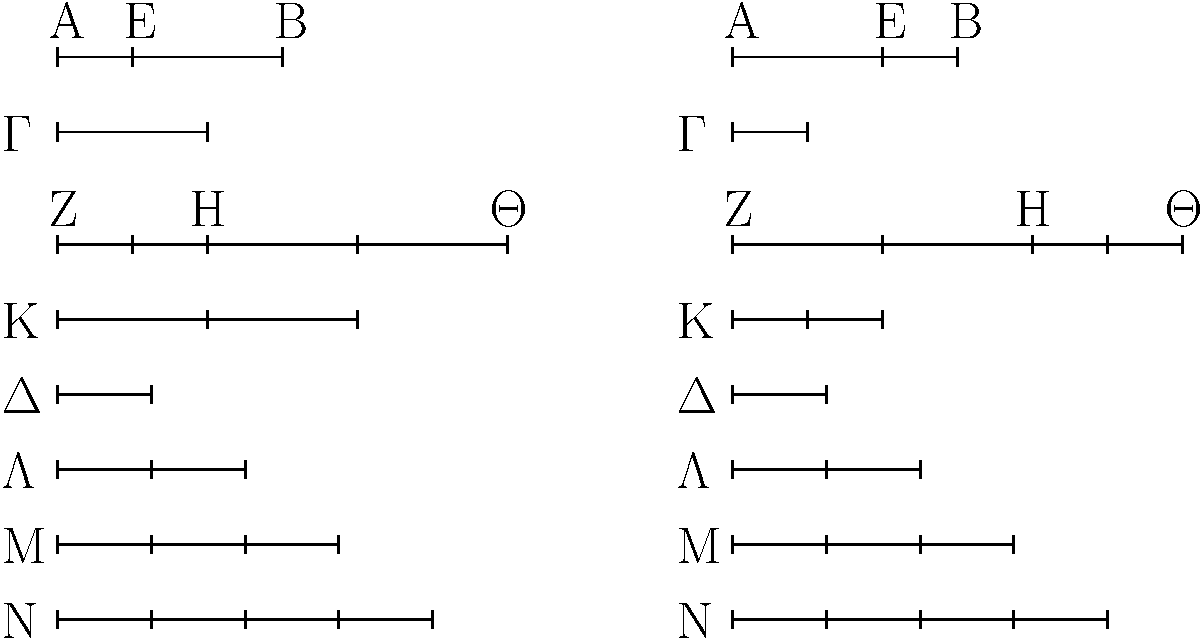
\includegraphics[width=0.8\textwidth]{Book05/fig08g.pdf}}

\gr{Ἐπεὶ γὰρ μεῖζόν ἐστι τὸ ΑΒ τοῦ Γ, κείσθω τῷ Γ ἴσον τὸ ΒΕ;
τὸ δὴ ὸέλασσον τῶν ΑΕ, ΕΒ πολλαπλασιαζόμενονὸέσται ποτὲ τοῦ
Δ μεῖζον. ὸέστω πρότερον τὸ ΑΕὸέλαττον τοῦ ΕΒ, καὶ πεπολλαπλασιάσθω
τὸ ΑΕ, καὶ ὸέστω αὐτοῦ πολλαπλάσιον τὸ ΖΗ μεῖζον ὃν τοῦ
Δ, καὶ ὁσαπλάσιόν ἐστι τὸ ΖΗ τοῦ ΑΕ, τοσαυταπλάσιον γεγονέτω
καὶ τὸ μὲν ΗΘ τοῦ ΕΒ τὸ δὲ Κ τοῦ Γ; καὶ εἰλήφθω τοῦ Δ 
διπλάσιον μὲν τὸ Λ, τριπλάσιον δὲ τὸ Μ, καὶ ἑχῆς ἑνὶ πλεῖον,
ὁέωςὸὰν τὸ λαμβανόμενον πολλαπλάσιον μὲν γένηται τοῦ Δ, 
πρώτως δὲ μεῖζον τοῦ Κ. εἰλήφθω, καὶ ὸέστω τὸ Ν τετραπλάσιον
μὲν τοῦ Δ, πρώτως δὲ μεῖζον τοῦ Κ.}

\gr{Ἐπεὶ οὸῦν τὸ Κ τοῦ Ν  πρώτως ἐστὶνὸέλαττον, τὸ Κ ἄρα τοῦ 
Μ οὸύκ ἐστινὸέλαττον. καὶ ἐπεὶ ἰσάκις ἐστὶ πολλαπλάσιον
τὸ ΖΗ τοῦ ΑΕ καὶ τὸ ΗΘ τοῦ ΕΒ, ἰσάκις ἄρα ἐστὶ πολλαπλάσιον
τὸ ΖΗ τοῦ ΑΕ καὶ τὸ ΖΘ τοῦ ΑΒ. ἰσάκις δέ ἐστι πολλαπλάσιον
τὸ ΖΗ τοῦ ΑΕ καὶ τὸ Κ τοῦ Γ; ἰσάκις ἄρα ἐστὶ πολλαπλάσιον
τὸ ΖΘ τοῦ ΑΒ καὶ τὸ Κ τοῦ Γ. τὰ ΖΘ, Κ ἄρα τῶν ΑΒ, Γ ἰσάκις
ἐστὶ πολλαπλάσια. πάλιν, ἐπεὶ ἰσάκις ἐστὶ πολλαπλάσιον τὸ ΗΘ 
τοῦ ΕΒ καὶ τὸ Κ τοῦ Γ,  ἴσον δὲ τὸ ΕΒ τῷ Γ,  ἴσον ἄρα
καὶ τὸ ΗΘ τῷ Κ. τὸ δὲ Κ τοῦ Μ οὸύκ ἐστινὸέλαττον; οὐδὸ
 ἄρα τὸ ΗΘ τοῦ Μὸέλαττόν ἐστιν. μεῖζον δὲ τὸ ΖΗ τοῦ Δ; ὅλον ἄρα τὸ ΖΘ συναμφοτέρων τῶν Δ, Μ μεῖζόν ἐστιν. ἀλλὰ συναμφότερα
τὰ Δ, Μ τῷ Ν ἐστιν ἴσα, ἐπειδήπερ τὸ Μ τοῦ Δ τριπλάσιόν
ἐστιν, συναμφότερα δὲ τὰ Μ, Δ τοῦ Δ ἐστι τετραπλάσια, ὸέστι
δὲ καὶ τὸ Ν τοῦ Δ τετραπλάσιον; συναμφότερα ἄρα τὰ Μ, Δ τῷ Ν ἴσα
ἐστίν. ἀλλὰ τὸ ΖΘ τῶν Μ, Δ μεῖζόν ἐστιν; τὸ ΖΘ ἄρα τοῦ Ν
ὑπερέθει; τὸ δὲ Κ τοῦ Ν οὐθ ὑπερέθει. καί ἐστι τὰ μὲν ΖΘ, Κ τῶν ΑΒ, Γ ἰσάκις πολλαπλάσια, τὸ δὲ Ν τοῦ Δὸάλλο, ὃ
ὸέτυθεν, πολλαπλάσιον; τὸ ΑΒ ἄρα πρὸς τὸ Δ μείζονα λόγον ἔχει ἢπερ τὸ Γ πρὸς τὸ Δ.}

\gr{Λέγω δή, ὅτι καὶ τὸ Δ πρὸς τὸ Γ μείζονα λόγον ἔχει ἢπερ
τὸ Δ πρὸς τὸ ΑΒ.}

\gr{Τῶν γὰρ αὐτῶν κατασκευασθέντων ὁμοίως δείχομεν, ὅτι
τὸ μὲν Ν τοῦ Κ ὑπερέθει, τὸ δὲ Ν τοῦ ΖΘ οὐθ ὑπερέθει.
καί ἐστι τὸ μὲν Ν τοῦ Δ πολλαπλάσιον, τὰ δὲ ΖΘ, Κ τῶν ΑΒ, Γὸάλλα, ὁὰ ὸέτυθεν, ἰσάκις πολλαπλάσια; τὸ Δ ἄρα πρὸς τὸ Γ
μείζονα λόγον ἔχει ἢπερ τὸ Δ πρὸς τὸ ΑΒ.}

\gr{Ἀλλὰ δὴ τὸ ΑΕ τοῦ ΕΒ μεῖζονὸέστω. τὸ δὴ ὸέλαττον τὸ ΕΒ
πολλαπλασιαζόμενονὸέσται ποτὲ τοῦ Δ μεῖζον. πεπολλαπλασιάσθω, καὶ
ὸέστω τὸ ΗΘ πολλαπλάσιον μὲν τοῦ ΕΒ, μεῖζον δὲ τοῦ Δ; καὶ
ὁσαπλάσιόν ἐστι τὸ ΗΘ τοῦ ΕΒ, τοσαυταπλάσιον γεγονέτω
καὶ τὸ μὲν ΖΗ τοῦ ΑΕ, τὸ δὲ Κ τοῦ Γ. ὁμοίως δὴ δείχομεν,
ὅτι τὰ ΖΘ, Κ τῶν ΑΒ, Γ ἰσάκις ἐστὶ πολλαπλάσια; καὶ εἰλήφθω
ὁμοίως τὸ Ν πολλαπλάσιον μὲν τοῦ Δ, πρώτως δὲ μεῖζον
τοῦ ΖΗ; ὁώστε πάλιν τὸ ΖΗ τοῦ Μ οὸύκ ἐστινὸέλασσον. μεῖζον
δὲ τὸ ΗΘ τοῦ Δ; ὅλον ἄρα τὸ ΖΘ τῶν Δ, Μ, τουτέστι τοῦ Ν,
ὑπερέθει. τὸ δὲ Κ τοῦ Ν οὐθ ὑπερέθει, ἐπειδήπερ καὶ τὸ
ΖΗ μεῖζον ὃν τοῦ ΗΘ, τουτέστι τοῦ Κ, τοῦ Ν οὐθ ὑπερέθει.
καὶ ὡσαύτως κατακολουθοῦντες τοῖς ἐπάνω περαίνομεν
τὴν ἀπόδειχιν.}

\gr{Τῶν ἄρα ἀνίσων μεγεθῶν τὸ μεῖζον πρὸς τὸ αὐτὸ μείζονα λόγον ἔχει ἢπερ τὸ ὸέλαττον; καὶ τὸ αὐτὸ πρὸς τὸ ὸέλαττον μείζονα
λόγον ἔχει ἢπερ πρὸς τὸ μεῖζον; ὅπερ ἔδει δεῖχαι.}}

\ParallelRText{
\begin{center}
{\large Proposition 8}
\end{center}

For unequal magnitudes, the greater (magnitude) has a greater
ratio  than the lesser to the same (magnitude). And the latter (magnitude)
has a greater ratio to the lesser (magnitude) than to the greater.

Let $AB$ and $C$ be unequal magnitudes, and let $AB$ be the greater (of the two),
and $D$ another random magnitude. I say that $AB$ has a greater ratio to $D$
than  $C$ (has) to $D$, and (that) $D$ has a greater ratio to $C$ than (it has) to $AB$.

% Removed epsf size command
\centerline{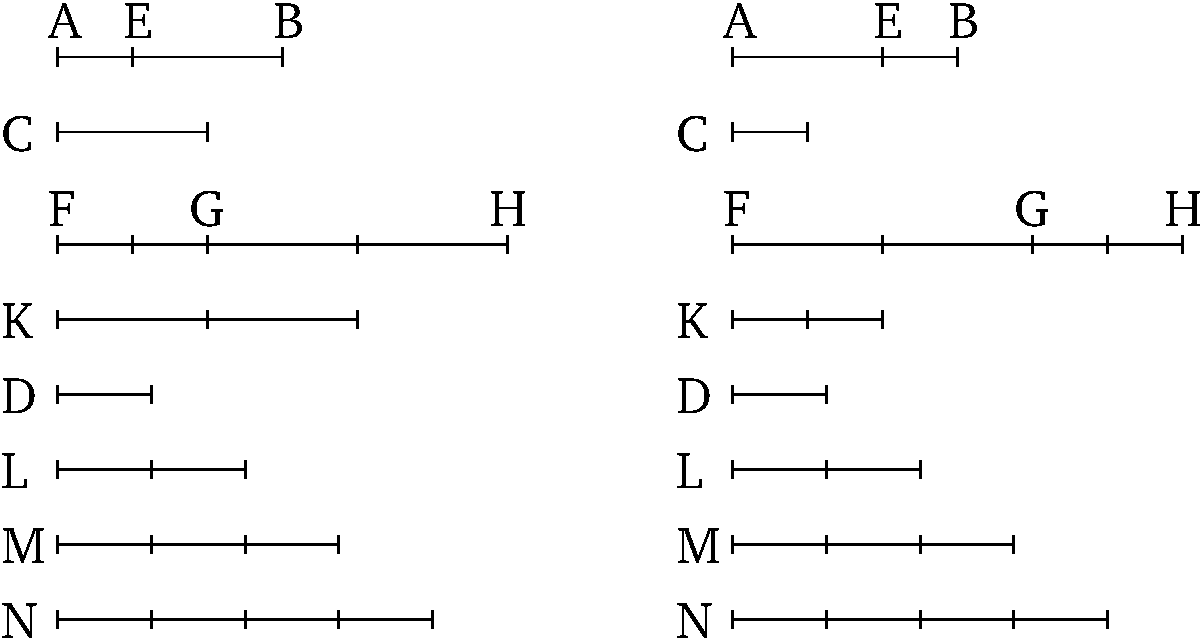
\includegraphics[width=0.8\textwidth]{Book05/fig08e.pdf}}

For since $AB$ is greater than $C$, let $BE$ be made equal to $C$.
So, the lesser of $AE$ and $EB$, being multiplied, will sometimes be greater than $D$ [Def.~5.4]. First of all, let $AE$ be less than $EB$, and let $AE$ be multiplied, 
and let $FG$ be a multiple of it which (is) greater than $D$.
And as many times as $FG$ is (divisible) by $AE$, so many times
let $GH$ also  become (divisible) by $EB$, and $K$ by $C$. And
let the double multiple $L$ of $D$ be taken, and the triple
multiple $M$, and several more, (each increasing) in order by one,
until the (multiple) taken  becomes the first multiple of $D$ (which is) greater than $K$. Let it be taken, and let it also be the quadruple multiple
$N$ of $D$---the first (multiple) greater than $K$.

Therefore, since $K$ is less than $N$ first, $K$ is thus not less than $M$.
And since $FG$ and $GH$ are equal multiples of $AE$ and $EB$ (respectively),
$FG$ and $FH$ are thus equal multiples of $AE$ and $AB$ (respectively) [Prop.~5.1].
And $FG$ and $K$ are equal multiples of $AE$ and $C$ (respectively).
Thus, $FH$ and $K$ are equal multiples of $AB$ and $C$ (respectively).
Thus, $FH$, $K$ are equal multiples of $AB$, $C$. Again, since $GH$ and 
$K$ are equal
multiples of $EB$ and $C$, and $EB$ (is) equal to $C$, $GH$ (is) thus also equal to
$K$. And $K$ is not less than $M$. Thus, $GH$ not less than $M$ either. And $FG$
(is) greater than $D$. Thus, the whole of $FH$ is greater than $D$
and $M$ (added) together. But, $D$ and $M$ (added) together is equal to $N$, 
inasmuch as $M$ is three times $D$, and $M$ and $D$ (added) together is four
times $D$, and $N$ is also four times $D$. Thus, $M$ and $D$ (added) together is
equal to $N$. But, $FH$ is greater than $M$ and $D$. Thus, $FH$ exceeds $N$. And $K$ does not exceed $N$. 
And $FH$, $K$  are equal multiples of $AB$, $C$, and $N$ another random multiple
of $D$. Thus, $AB$ has a greater ratio to $D$  than $C$ (has) to $D$ [Def.~5.7].

So, I say that $D$ also has a greater ratio to $C$ than $D$ (has) to $AB$.

For, similarly, by the same construction, we can show that 
$N$ exceeds $K$, and $N$ does not exceed $FH$. And $N$ is a multiple of $D$,
and $FH$, $K$ other  random  equal multiples of $AB$, $C$ (respectively). Thus, $D$ has a greater
ratio to  $C$ than $D$ (has) to $AB$ [Def.~5.5].

And so let $AE$ be greater than $EB$. So, the lesser, $EB$, being multiplied, will
sometimes be greater than $D$. Let it be multiplied, and let $GH$ be
a multiple of $EB$ (which is) greater than $D$. And as many times as $GH$ is
(divisible) by $EB$, so many times let $FG$ also  become (divisible) by $AE$,
and $K$ by $C$. So, similarly (to the above), we can show that $FH$ and $K$ are equal multiples of
$AB$ and $C$ (respectively). And, similarly (to the above), let the multiple $N$ of $D$,  (which is)
the first (multiple) greater than $FG$, be taken. So,  $FG$ is again not less than $M$.
And $GH$ (is) greater than $D$. Thus, the whole of $FH$ exceeds $D$ and $M$, that is to say $N$.  And $K$ does not exceed $N$, inasmuch as $FG$, which (is) greater than
$GH$---that is to say, $K$---also does not exceed $N$. And, following the above (arguments), we  (can) complete the proof in the same manner.

Thus, for unequal magnitudes, the greater (magnitude) has a greater
ratio  than the lesser to the same (magnitude). And the latter (magnitude)
has a greater ratio to the lesser (magnitude) than to the greater. (Which is)
the very thing it was required to show.}
\end{Parallel}

%%%%%%
% Prop 5.9
%%%%%%
\pdfbookmark[1]{Proposition 5.9}{pdf5.9}
\begin{Parallel}{}{} 
\ParallelLText{
\begin{center}
{\large \ggn{9}.}
\end{center}\vspace*{-7pt}

\gr{Τὰ πρὸς τὸ αὐτὸ τὸν αὐτὸν ἔχοντα λὸγον ἴσα ἀλλήλοις ἐστίν;
καὶ πρὸς ὁὰ τὸ αὐτὸ τὸν αὐτὸν ὁέθει λόγον, ἐκεῖνα ἴσα ἐστίν.}

% Removed epsf size command
\centerline{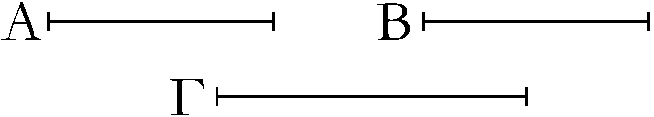
\includegraphics[width=0.8\textwidth]{Book05/fig09g.pdf}}

\gr{Ἐθέτω γὰρ ἑκάτερον τῶν Α, Β πρὸς τὸ Γ τὸν αὐτὸν λόγον;
λέγω, ὅτι ἴσον ἐστὶ τὸ Α τῷ Β.}

\gr{Εἰ γὰρ μή, οὐκὸὰν ἑκάτερον τῶν Α, Β πρὸς τὸ Γ τὸν αὐτὸν
εὸῖθε λόγον;  ἔχει δέ;  ἴσον ἄρα ἐστὶ τὸ Α τῷ Β.}

\gr{Ἐθέτω δὴ πάλιν τὸ Γ πρὸς ἑκάτερον τῶν Α, Β τὸν αὐτὸν
λόγον; λέγω, ὅτι ἴσον ἐστὶ τὸ Α τῷ Β.}

\gr{Εἰ γὰρ μή, οὐκὸὰν τὸ Γ πρὸς ἑκάτερον τῶν Α, Β τὸν αὐτὸν εὸῖθε λόγον;  ἔχει δέ;  ἴσον ἄρα ἐστὶ τὸ Α τῷ Β.}

\gr{Τὰ  ἄρα πρὸς τὸ αὐτὸ τὸν αὐτὸν ἔχοντα λόγον ἴσα ἀλλήλοις
ἐστίν; καὶ πρὸς ὁὰ τὸ αὐτὸ τὸν αὐτὸν ἔχει λόγον, ἐκεῖνα ἴσα ἐστίν; ὅπερ ἔδει δεῖχαι.}}

\ParallelRText{
\begin{center}
{\large Proposition 9}
\end{center}

(Magnitudes) having the same ratio to the same (magnitude) are equal to one another. And those (magnitudes) to which the same (magnitude)
has the same ratio are equal.

% Removed epsf size command
\centerline{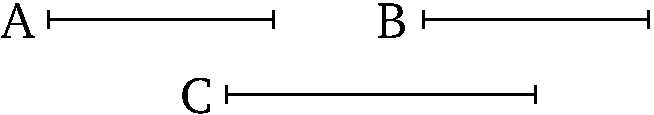
\includegraphics[width=0.8\textwidth]{Book05/fig09e.pdf}}

For let $A$ and $B$ each have the same ratio to $C$. I say that $A$ is equal to $B$.

For if not, $A$ and $B$ would not each have the same ratio to $C$ [Prop.~5.8].
But they do. Thus, $A$ is equal to $B$.

So, again, let $C$ have the same ratio to each of $A$ and $B$. I say that $A$ is equal to $B$.

For if not, $C$ would not have the same ratio to each of $A$ and $B$ [Prop.~5.8]. But it does. Thus, $A$ is equal to $B$.

Thus, (magnitudes) having the same ratio to the same (magnitude) are equal to one another. And those (magnitudes) to which the same (magnitude)
has the same ratio are equal. (Which is) the very thing it was required to show.}
\end{Parallel}

%%%%%%
% Prop 5.10
%%%%%%
\pdfbookmark[1]{Proposition 5.10}{pdf5.10}
\begin{Parallel}{}{} 
\ParallelLText{
\begin{center}
{\large \ggn{10}.}
\end{center}\vspace*{-7pt}

\gr{Τῶν πρὸς τὸ αὐτὸ λόγον ἐθόντων τὸ μείζονα λόγον ἔχον ἐκεῖνο μεῖζόν ἐστιν; πρὸς ὃ δὲ τὸ αὐτὸ μείζονα λόγον ἔχει, ἐκεῖνοὸέλαττόν ἐστιν.}\\

% Removed epsf size command
\centerline{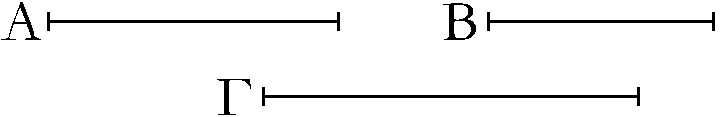
\includegraphics[width=0.8\textwidth]{Book05/fig10g.pdf}}

\gr{Ἐθέτω γὰρ τὸ Α πρὸς τὸ Γ μείζονα λόγον ἢπερ τὸ Β πρὸς τὸ Γ;
λέγω, ὅτι μεῖζόν ἐστι τὸ Α  τοῦ Β.}

\gr{Εἰ γὰρ μή,  ἢτοι ἴσον ἐστὶ τὸ Α τῷ Βὸὴ ὸέλασσον.  ἴσον
μὲν οὸῦν οὸύκ ἐστὶ τὸ Α τῷ Β; ἑκάτερον γὰρὸὰν τῶν Α, Β
πρὸς τὸ Γ τὸν αὐτὸν εὸῖθε λόγον. οὐκ ἔχει δέ; οὐκ ἄρα ἴσον
ἐστὶ τὸ Α τῷ Β. οὐδὲ μὴνὸέλασσόν ἐστι τὸ Α τοῦ Β; τὸ Α γὰρὸὰν πρὸς τὸ Γ  ἐλάσσονα λόγον εὸῖθεν ἢπερ τὸ Β πρὸς τὸ Γ. οὐκ ἔχει δέ; οὐκ ἄραὸέλασσόν ἐστι τὸ Α τοῦ Β. ἐδείθθη δὲ οὐδὲ  ἴσον; μεῖζον ἄρα ἐστὶ τὸ Α τοῦ Β.}

\gr{Ἐθέτω δὴ πάλιν τὸ Γ πρὸς τὸ Β μείζονα λόγον ἢπερ τὸ Γ πρὸς
τὸ Α; λέγω, ὅτιὸέλασσόν ἐστι τὸ Β τοῦ Α.}

\gr{Εἰ γὰρ μή,  ἢτοι ἴσον ἐστὶνὸὴ μεῖζον.  ἴσον μὲν οὸῦν οὸύκ
ἐστι τὸ Β τῷ Α; τὸ Γ γὰρὸὰν πρὸς ἑκάτερον τῶν Α, Β τὸν αὐτὸν
εὸῖθε λόγον. οὐκ ἔχει δέ; οὐκ ἄρα ἴσον ἐστὶ τὸ Α τῷ Β. οὐδὲ
μὴν μεῖζόν ἐστι τὸ Β τοῦ Α; τὸ Γ γὰρὸὰν πρὸς τὸ Β ἐλάσσονα
λόγον εὸῖθεν ἢπερ πρὸς τὸ Α. οὐκ ἔχει δέ; οὐκ ἄρα
μεῖζόν ἐστι τὸ Β τοῦ Α. ἐδείθθη δέ, ὅτι οὐδὲ  ἴσον; ὸέλαττον ἄρα ἐστὶ τὸ Β τοῦ Α.}

\gr{Τῶν ἄρα  πρὸς τὸ αὐτὸ λόγον ἐθόντων τὸ μείζονα λόγον ἔχον μεῖζόν ἐστιν; καὶ πρὸς ὃ  τὸ αὐτὸ μείζονα λόγον ἔχει, ἐκεῖνοὸέλαττόν ἐστιν; ὅπερ ἔδει δεῖχαι.}}

\ParallelRText{
\begin{center}
{\large Proposition 10}
\end{center}

For (magnitudes) having a ratio to the same (magnitude), that (magnitude which) has the
greater ratio is (the) greater. And that (magnitude) to which the latter (magnitude) has a greater ratio is (the)
lesser.

% Removed epsf size command
\centerline{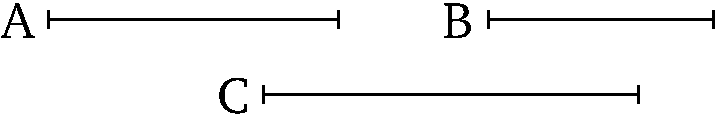
\includegraphics[width=0.8\textwidth]{Book05/fig10e.pdf}}

For let $A$ have a greater ratio to $C$ than $B$ (has) to $C$. I say that $A$ is greater than $B$.

For if not, $A$ is surely either equal to or less than $B$. In fact, $A$ is not
equal to $B$. For (then) $A$ and $B$ would each have the same ratio to $C$ 
 [Prop.~5.7]. But they do not. Thus, $A$
 is not equal to $B$. Neither, indeed, is $A$ less than $B$. For (then)
 $A$ would have a lesser ratio to $C$ than $B$ (has) to $C$ [Prop.~5.8]. But it does not. Thus, $A$ is not less
 than $B$. And it was shown not (to be) equal either. Thus, $A$ is greater than $B$.
 
 So, again, let $C$ have a greater ratio to $B$ than $C$ (has) to $A$. I say that
 $B$ is less than $A$.
 
 For if not, (it is) surely either equal or greater. In fact, $B$ is not equal to 
 $A$. For (then) $C$ would have the same ratio to each of $A$ and $B$  [Prop.~5.7]. But it does not. Thus, $A$ is not equal to $B$. 
 Neither, indeed, is $B$ greater than $A$. For (then) $C$ would have a lesser
 ratio to $B$ than (it has) to $A$ [Prop.~5.8].
 But it does not. Thus, $B$ is not greater than $A$. And it was shown that
  (it is) not equal (to $A$) either. Thus, $B$ is less than $A$.
  
 Thus, for (magnitudes) having a ratio to the same (magnitude), that (magnitude which)
 has the greater  ratio is (the) greater. And that (magnitude) to which the latter (magnitude) has a greater ratio is (the)
lesser. (Which is) the very thing it was required to show.}
\end{Parallel}

%%%%%%
% Prop 5.11
%%%%%%
\pdfbookmark[1]{Proposition 5.11}{pdf5.11}
\begin{Parallel}{}{} 
\ParallelLText{
\begin{center}
{\large \ggn{11}.}
\end{center}\vspace*{-7pt}

\gr{Οἱ τῷ αὐτῷ λόγῳ οἱ αὐτοὶ καὶ ἀλλήλοις εἰσὶν οἱ αὐτοί.}

\gr{Ἔστωσαν γὰρ ὡξ μὲν τὸ Α πρὸς τὸ Β, οὁύτως τὸ Γ πρὸς τὸ Δ, ὡξ
δὲ τὸ Γ πρὸς τὸ Δ, οὁύτως τὸ Ε πρὸς τὸ Ζ; λέγω, ὅτι ἐστὶν ὡξ
τὸ Α πρὸς τὸ Β, οὁύτως τὸ Ε πρὸς τὸ Ζ.}

\gr{Εἰλήφθω γὰρ τῶν Α, Γ, Ε ἰσάκις πολλαπλάσια τὰ Η, Θ, Κ, τῶν δὲ Β, Δ, Ζὸάλλα, ὁὰ ὸέτυθεν, ἰσάκις πολλαπλάσια τὰ Λ, Μ, Ν.}

% Removed epsf size command
\centerline{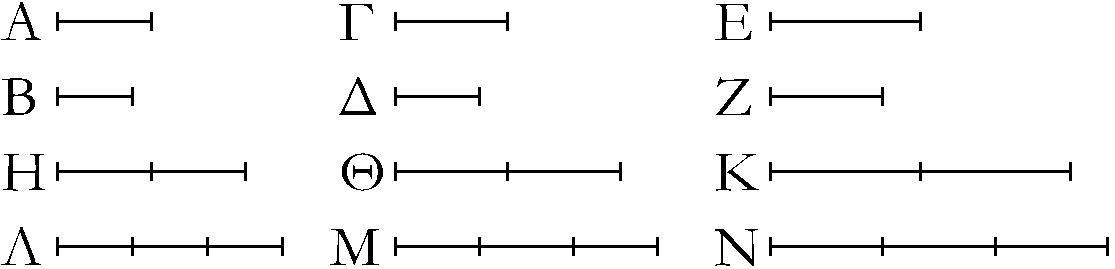
\includegraphics[width=0.8\textwidth]{Book05/fig11g.pdf}}

\gr{Καὶ ἐπεί ἐστιν ὡξ τὸ Α πρὸς τὸ Β, οὁύτως τὸ Γ
πρὸς τὸ Δ, καὶ εὸίληπται τῶν μὲν Α, Γ ἰσάκις πολλαπλάσια τὰ Η, Θ,
τῶν δὲ Β, Δὸάλλα, ὁὰ ὸέτυθεν, ἰσάκις πολλαπλάσια τὰ Λ, Μ, εἰ
 ἄρα ὑπερέθει τὸ Η τοῦ Λ, ὑπερέθει καὶ τὸ Θ τοῦ Μ, καὶ εἰ
 ἴσον ἐστίν,  ἴσον, καὶ εἰ ἐλλείπει, ἐλλείπει. πάλιν, ἐπεί
ἐστιν ὡξ τὸ Γ πρὸς τὸ Δ, οὁύτως τὸ Ε πρὸς τὸ Ζ, καὶ εὸίληπται
τῶν  Γ, Ε ἰσάκις πολλαπλάσια τὰ Θ, Κ, τῶν δὲ Δ, Ζὸάλλα, ὁὰ ὸέτυθεν,
ἰσάκις πολλαπλάσια τὰ Μ, Ν, εἰ  ἄρα ὑπερέθει τὸ Θ τοῦ Μ,
ὑπερέθει καὶ τὸ Κ τοῦ Ν, καὶ εἰ  ἴσον,  ἴσον, καὶ εἰ
ὸέλλατον, ὸέλαττον. ἀλλὰ εἰ ὑπερεῖθε τὸ Θ τοῦ Μ, ὑπερεῖθε
καὶ τὸ Η τοῦ Λ, καὶ εἰ  ἴσον,  ἴσον, καὶ εἰ ὸέλαττον, 
ὸέλαττον; ὁώστε καὶ εἰ ὑπερέθει τὸ Η τοῦ Λ, ὑπερέθει καὶ τὸ
Κ τοῦ Ν, καὶ εἰ  ἴσον,  ἴσον, καὶ εἰ ὸέλαττον, ὸέλαττον. καί
ἐστι τὰ  μὲν Η, Κ τῶν Α, Ε ἰσάκις πολλαπλάσια, τὰ δὲ Λ, Ν τῶν
Β, Ζὸάλλα, ὁὰ ὸέτυθεν, ἰσάκις πολλαπλάσια; ὸέστιν ἄρα ὡξ τὸ Α πρὸς
τὸ Β, οὁύτως τὸ Ε πρὸς τὸ Ζ.}

\gr{Οἱ  ἄρα τῷ αὐτῷ λόγῳ οἱ αὐτοὶ καὶ ἀλλήλοις εἰσὶν οἱ αὐτοί;
ὅπερ ἔδει δεῖχαι.}}

\ParallelRText{
\begin{center}
{\large Proposition 11}$^\dag$
\end{center}

(Ratios which are) the same with the same ratio  are also the same with one another.

For let it be that as $A$ (is) to $B$, so $C$ (is) to $D$, and as $C$ (is) to $D$, so $E$ (is) to $F$. I say
that as  $A$ is to $B$, so $E$ (is) to $F$.

For let the equal multiples $G$, $H$,  $K$ be taken of $A$, $C$,  $E$ (respectively), and
the other random equal multiples $L$, $M$,  $N$ of $B$, $D$, $F$ (respectively).

% Removed epsf size command
\centerline{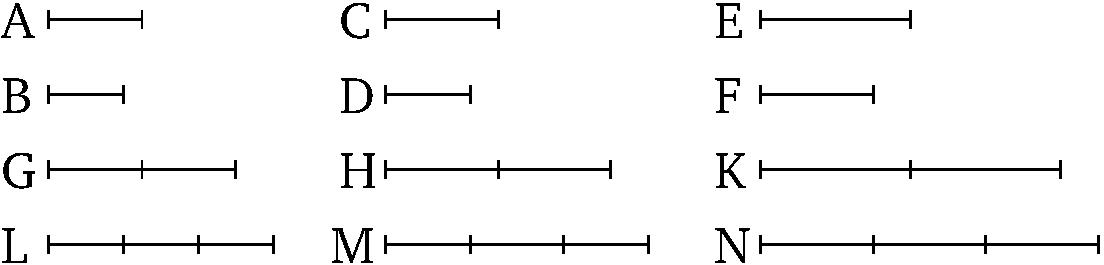
\includegraphics[width=0.8\textwidth]{Book05/fig11e.pdf}}

And since as $A$ is to $B$, so $C$ (is) to $D$, and the equal multiples $G$ and $H$
be taken of $A$ and $C$ (respectively), and the other random equal
multiples $L$ and $M$ of $B$ and $D$ (respectively),  thus if $G$ exceeds $L$ (then)
$H$ also exceeds $M$, and if ($G$ is) equal (to $L$ then $H$ is also)
equal (to $M$), and if ($G$ is) less (than $L$ then $H$ is also) less (than $M$)  [Def.~5.5]. Again, since as $C$ is to $D$, so $E$
(is) to $F$, and the equal multiples $H$ and $K$ have been taken of $C$ and $E$
(respectively), and the other random equal multiples $M$ and $N$ of
$D$ and $F$ (respectively), thus if $H$ exceeds $M$ (then)
$K$ also exceeds $N$, and if ($H$ is) equal  (to $M$ then $K$ is also)
equal (to $N$), and if ($H$ is) less (than $M$  then $K$ is also) less (than $N$) [Def.~5.5]. But (we saw that) if $H$ was exceeding $M$ (then) $G$ was also
exceeding $L$, and if ($H$ was) equal (to $M$ then $G$ was also)
equal (to $L$), and if ($H$ was) less (than $M$ then $G$ was also) less (than $L$).
And, hence, if $G$ exceeds $L$ (then)
$K$ also exceeds $N$, and if ($G$ is) equal (to $L$ then $K$ is also)  equal (to $N$), and if ($G$ is) less (than $L$ then $K$ is also) less (than $N$). And $G$ and $K$ are equal multiples of $A$ and $E$ (respectively), and $L$ and $N$
other random equal multiples of $B$ and $F$ (respectively). Thus, as $A$ is to $B$,
so $E$ (is) to $F$ [Def.~5.5].

Thus, (ratios which are) the same with the same ratio  are also the same with one another. (Which is) the very thing it was required to show.}
\end{Parallel}
{\footnotesize \noindent$^\dag$ In modern notation, this proposition
reads that if $\alpha:\beta::\gamma:\delta$ and $\gamma:\delta::\epsilon:\zeta$ then $\alpha:\beta::\epsilon:\zeta$.}

%%%%%%
% Prop 5.12
%%%%%%
\pdfbookmark[1]{Proposition 5.12}{pdf5.12}
\begin{Parallel}{}{} 
\ParallelLText{
\begin{center}
{\large \ggn{12}.}
\end{center}\vspace*{-7pt}

\gr{Ἐὰνὸῆ| ὁποσαοῦν μεγέθη  ἀνάλογον, ὸέσται ὡξ ὁὲν τῶν ἡγουμένων πρὸς ὁὲν τῶν ἑπομένων, οὁύτως ὁάπαντα τὰ ἡγούμενα πρὸς ὁάπαντα τὰ ἑπόμενα.}\\

% Removed epsf size command
\centerline{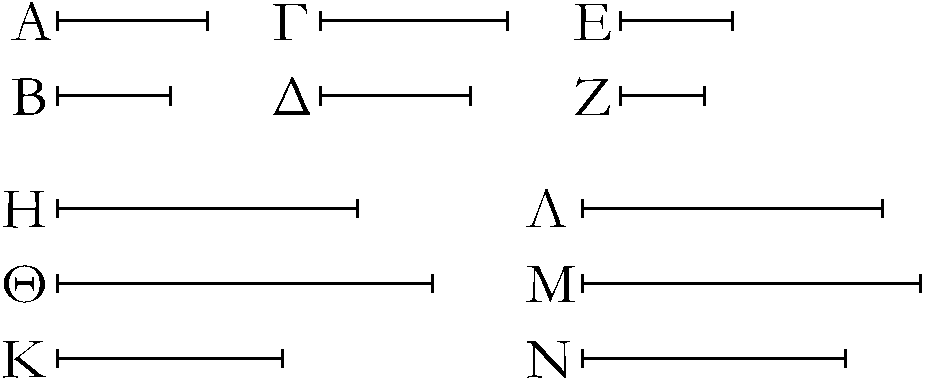
\includegraphics[width=0.8\textwidth]{Book05/fig12g.pdf}}

\gr{Ἔστωσαν ὁποσαοῦν μεγέθη ἀνάλογον τὰ Α, Β, Γ, Δ, Ε, Ζ, ὡξ τὸ
Α πρὸς τὸ Β, οὁύτως τὸ Γ πρὸς τὸ Δ, καὶ τὸ Ε πρὸς το Ζ; λέγω, ὅτι
ἐστὶν ὡξ τὸ Α πρὸς τὸ Β, οὁύτως τὰ Α, Γ, Ε πρὸς τὰ Β, Δ, Ζ.}

\gr{Εἰλήφθω γὰρ τῶν μὲν Α, Γ, Ε ἰσάκις πολλαπλάσια τὰ Η, Θ, Κ, τῶν
δὲ Β, Δ, Ζὸάλλα, ὁὰ ὸέτυθεν, ἰσάκις πολλαπλάσια τὰ Λ, Μ, Ν.}

\gr{Καὶ ἐπεί ἐστιν ὡξ τὸ Α πρὸς τὸ Β, οὁύτως τὸ Γ πρὸς τὸ Δ, καὶ
τὸ Ε πρὸς τὸ Ζ, καὶ εὸίληπται τῶν μὲν Α, Γ, Ε ἰσάκις πολλαπλάσια
τὰ Η, Θ, Κ τῶν δὲ Β, Δ, Ζὸάλλα, ὁὰ ὸέτυθεν, ἰσάκις πολλαπλάσια
τὰ Λ, Μ, Ν, εἰ  ἄρα ὑπερέθει τὸ Η τοῦ Λ, ὑπερέθει καὶ τὸ Θ
τοῦ Μ, καὶ τὸ Κ τοῦ Ν, καὶ εἰ  ἴσον,  ἴσον, καὶ εἰ ὸέλαττον, ὸέλαττον.
ὁώστε καὶ εἰ ὑπερέθει τὸ Η τοῦ Λ, ὑπερέθει καὶ τὰ Η, Θ, Κ τῶν
Λ, Μ, Ν,  καὶ εἰ  ἴσον,  ἴσα, καὶ εἰ ὸέλαττον, ὸέλαττονα. καί ἐστι
τὸ μὲν Η καὶ τὰ Η, Θ, Κ τοῦ Α καὶ τῶν Α, Γ, Ε ἰσάκις
πολλαπλάσια, ἐπειδήπερ ἒανὸῆ|  ὁποσαοῦν μεγέθη ὁποσωνοῦν
μεγεθῶνὸίσων τὸ πλῆθος ὁέκαστον ἑκάστου ἰσάκις πολλαπλάσιον,
ὁσαπλάσιόν ἐστιν ὁὲν τῶν μεγεθῶν ἑνόξ, τοσαυταπλάσιαὸέσται
καὶ τὰ πάντα τῶν πάντων. διὰ τὰ αὐτὰ δὴ καὶ τὸ Λ καὶ τὰ Λ, Μ, Ν
τοῦ Β καὶ τῶν Β, Δ, Ζ ἰσάκις ἐστὶ πολλαπλάσια;
ὸέστιν ἄρα ὡξ τὸ Α πρὸς τὸ Β, οὁύτως τὰ Α, Γ, Ε πρὸς τὰ Β, Δ, Ζ.}

\gr{Ἐὰν ἄραὸῆ| ὁποσαοῦν μεγέθη  ἀνάλογον, ὸέσται ὡξ ὁὲν τῶν ἡγουμένων πρὸς ὁὲν τῶν ἑπομένων, οὁύτως ὁάπαντα τὰ ἡγούμενα πρὸς ὁάπαντα τὰ ἑπόμενα; ὅπερ ἔδει δεῖχαι.}}

\ParallelRText{
\begin{center}
{\large Proposition 12}$^\dag$
\end{center}

If there are any number  of magnitudes whatsoever
(which are) proportional, (then) as one of the leading (magnitudes is) to one of the following, so
will 
all of the leading (magnitudes) be to all of the following.

% Removed epsf size command
\centerline{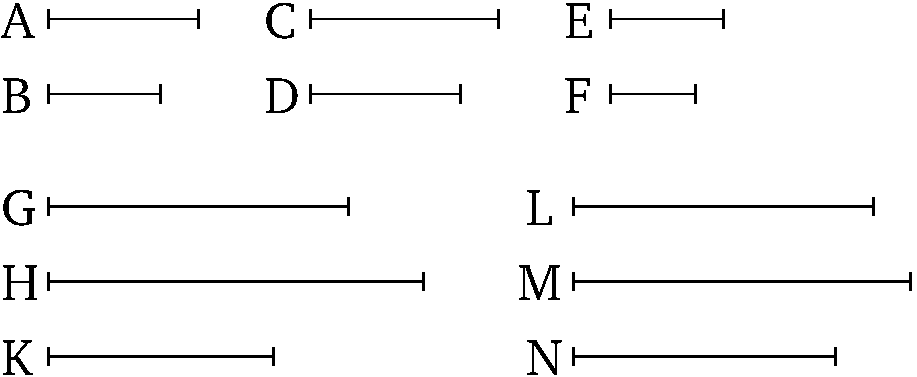
\includegraphics[width=0.8\textwidth]{Book05/fig12e.pdf}}

Let there be any number of magnitudes whatsoever, 
$A$, $B$, $C$, $D$, $E$, $F$, (which are) proportional, (so that) as $A$ (is) to $B$, so $C$ (is) to $D$, and 
$E$ to $F$. I say that as $A$ is to $B$, so  $A$, $C$, $E$ (are) to  $B$, $D$, $F$.

For let the equal multiples $G$, $H$,  $K$ be taken of $A$, $C$, $E$
(respectively), and the other random equal multiples $L$, $M$,  $N$ of
$B$, $D$, $F$ (respectively).

And since as $A$ is to $B$, so $C$ (is) to $D$, and $E$ to $F$, and the equal multiples
$G$, $H$, $K$ have been taken of $A$, $C$,  $E$ (respectively), and the other
random equal multiples $L$, $M$,  $N$ of $B$, $D$,  $F$ (respectively), thus
if $G$ exceeds $L$ (then) $H$ also exceeds $M$, and $K$ (exceeds) $N$, and if ($G$ is)
equal (to $L$ then $H$ is also) equal (to $M$, and $K$  to $N$), and if ($G$ is) less (than $L$ then $H$ is also) less (than $M$, and $K$  than $N$)  [Def.~5.5].  And, hence, if $G$ exceeds $L$ (then)
$G$, $H$, $K$ also exceed $L$, $M$, $N$, and if ($G$ is) equal
(to $L$ then $G$, $H$, $K$ are also) equal (to  $L$, $M$, $N$) and if ($G$ is) less (than $L$ then
$G$, $H$, $K$ are also) less (than $L$, $M$, $N$). And $G$ and $G$, $H$, $K$ are equal multiples
of $A$ and $A$, $C$, $E$ (respectively), inasmuch as if there are any number of magnitudes whatsoever (which are)  equal multiples, respectively, of
some  (other) magnitudes,  of equal  number (to them), (then) as many times as one of the (first) magnitudes is (divisible) by one (of the second), so many times
will all (of the first magnitudes) also (be divisible) by all (of the second)
 [Prop.~5.1]. So, for the same (reasons), $L$
 and $L$, $M$, $N$ are also equal multiples of $B$ and $B$, $D$, $F$ (respectively). Thus,
 as $A$ is to $B$, so $A$, $C$, $E$ (are) to $B$, $D$, $F$ (respectively).
 
Thus, if there are any number  of magnitudes whatsoever
(which are) proportional, (then) as one of the leading (magnitudes is) to one of the following, so
will 
all of the leading (magnitudes) be to all of the following. (Which is) the
very thing it was required to show.}
\end{Parallel}
{\footnotesize \noindent$^\dag$ In modern notation, this proposition
reads that if $\alpha:\alpha'::\beta:\beta'::\gamma:\gamma'$ {\rm etc.}\ then
$\alpha:\alpha'::(\alpha+\beta+\gamma+\cdots):(\alpha'+\beta'+\gamma'+\cdots)$.}

%%%%%%
% Prop 5.13
%%%%%%
\pdfbookmark[1]{Proposition 5.13}{pdf5.13}
\begin{Parallel}{}{} 
\ParallelLText{
\begin{center}
{\large \ggn{13}.}
\end{center}\vspace*{-7pt}

\gr{Ἐὰν πρῶτον πρὸς δεύτερον τὸν αὐτὸνὸὲθῃ  λόγον καὶ τρίτον
πρὸς τέταρτον, τρίτον δὲ πρὸς τέταρτον μείζονα λόγονὸέθῃ ὸὴ πέμπτον
πρὸς ὁέκτον, καὶ πρῶτον πρὸς δεύτερον μείζονα λόγον ὁέχειὸὴ
πέμπτον πρὸς ὁέκτον.}\\

% Removed epsf size command
\centerline{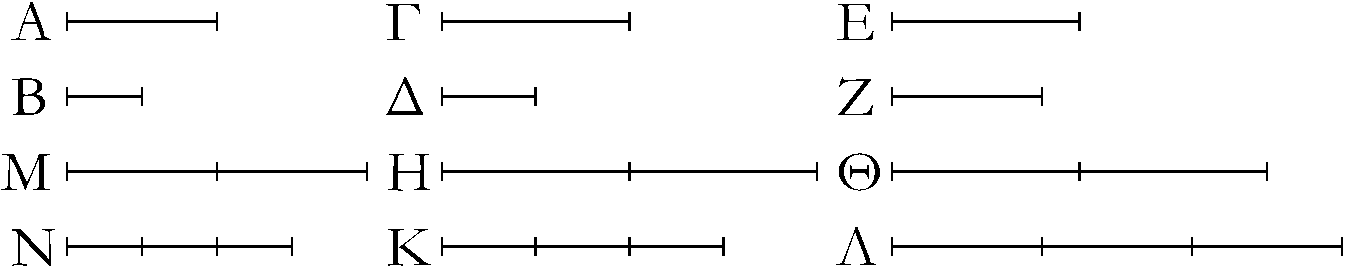
\includegraphics[width=0.8\textwidth]{Book05/fig13g.pdf}}

\gr{Πρῶτον γὰρ τὸ Α πρὸς δεύτερον τὸ Β τὸν αὐτὸν ἐθέτω λόγον καὶ
τρίτον τὸ Γ πρὸς τέταρτον τὸ Δ, τρίτον δὲ τὸ Γ πρὸς τέταρτον τὸ Δ
μείζονα λόγον ἐθέτωὸὴ πέμπτον τὸ Ε πρὸς ὁέκτον τὸ Ζ. λέγω,
ὅτι καὶ πρῶτον τὸ Α πρὸς δεύτερον τὸ Β μείζονα λόγον ὁέχει ἢπερ πέμπτον τὸ Ε πρὸς ὁέκτον τὸ Ζ.}

\gr{Ἐπεὶ γὰρὸέστι τινὰ τῶν μὲν Γ, Ε ἰσάκις πολλαπλάσια, τῶν δὲ Δ, Ζὸάλλα, ὁὰ ὸέτυθεν, ἰσάκις πολλαπλάσια, καὶ τὸ μὲν τοῦ Γ πολλαπλάσιον
τοῦ τοῦ Δ πολλαπλασίου ὑπερέθει, τὸ δὲ τοῦ Ε πολλαπλάσιον τοῦ τοῦ Ζ
πολλαπλασίου οὐθ ὑπερέθει, εἰλήφθω, καὶ ὸέστω τῶν μὲν Γ, Ε ἰσάκις
πολλαπλάσια τὰ Η, Θ, τῶν δὲ Δ, Ζὸάλλα, ὁὰ ὸέτυθεν, ἰσάκις πολλαπλάσια
τὰ Κ, Λ, ὁώστε τὸ μὲν Η τοῦ Κ ὑπερέθειν, τὸ δὲ Θ τοῦ Λ μὴ
ὑπερέθειν; καὶ ὁσαπλάσιον μέν ἐστι τὸ Η τοῦ Γ, τοσαυταπλάσιονὸέστω καὶ τὸ Μ τοῦ Α, ὁσαπλάσιον δὲ τὸ Κ τοῦ Δ, τοσαυταπλάσιονὸέστω καὶ τὸ Ν τοῦ Β.}

\gr{Καὶ ἐπεί ἐστιν ὡξ τὸ Α πρὸς τὸ Β, οὁύτως τὸ Γ πρὸς τὸ Δ, καὶ
εὸίληπται τῶν μὲν Α, Γ ἰσάκις πολλαπλάσια τὰ Μ, Η, τῶν δὲ Β, Δὸάλλα, ὁὰ ὸέτυθεν, ἰσάκις πολλαπλάσια τὰ Ν, Κ, εἰ  ἄρα ὑπερέθει
τὸ Μ τοῦ Ν, ὑπερέθει καὶ τὸ Η τοῦ Κ, καὶ εἰ  ἴσον,  ἴσον,
καὶ εἰ ὸέλαττον, ὸέλλατον. ὑπερέθει δὲ τὸ Η τοῦ Κ; ὑπερέθει ἄρα καὶ τὸ Μ τοῦ Ν. τὸ δὲ Θ τοῦ Λ οὐθ ὑπερέθει; καί
ἐστι τὰ μὲν Μ, Θ τῶν Α, Ε ἰσάκις πολλαπλάσια, τὰ δὲ Ν, Λ τῶν
Β, Ζὸάλλα, ὁὰ ὸέτυθεν, ἰσάκις πολλαπλάσια; τὸ  ἄρα Α πρὸς
τὸ Β μείζονα λόγον ἔχει ἢπερ τὸ Ε πρὸς τὸ Ζ.}

\gr{Ἐὰν ἄρα πρῶτον πρὸς δεύτερον τὸν αὐτὸνὸὲθῃ  λόγον καὶ τρίτον
πρὸς τέταρτον, τρίτον δὲ πρὸς τέταρτον μείζονα λόγονὸέθῃ ὸὴ πέμπτον
πρὸς ὁέκτον, καὶ πρῶτον πρὸς δεύτερον μείζονα λόγον ὁέχειὸὴ
πέμπτον πρὸς ὁέκτον; ὅπερ ἔδει δεῖχαι.}}

\ParallelRText{
\begin{center}
{\large Proposition 13}$^\dag$
\end{center}

If a first (magnitude) has the same ratio to a second that a third (has) to a fourth, and the third (magnitude) has a greater ratio to the fourth than a fifth (has) to a sixth, (then) the first (magnitude) will also have a greater ratio to the
second  than the fifth (has) to the sixth.

% Removed epsf size command
\centerline{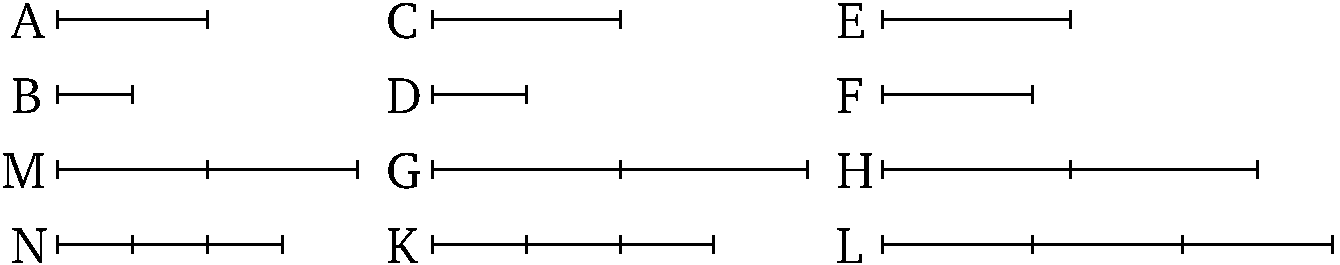
\includegraphics[width=0.8\textwidth]{Book05/fig13e.pdf}}

For let a first (magnitude) $A$ have the same ratio to a second $B$ that a
third $C$ (has) to a fourth $D$, and let the third (magnitude) $C$ have a
greater ratio to the fourth $D$  than a fifth $E$ (has) to a sixth $F$. I say that the first (magnitude) $A$
will also have a greater ratio to the second $B$ than the fifth $E$ (has) to the
sixth $F$.

For since there are some equal multiples of $C$ and $E$, and other random equal multiples of $D$ and $F$, (for which) the multiple of $C$ exceeds the (multiple) of $D$, 
and the multiple of $E$ does not exceed the multiple of $F$ [Def.~5.7], let them be taken. And let
$G$ and $H$ be equal multiples of $C$ and $E$ (respectively), and $K$ and $L$
other random equal multiples of $D$ and $F$ (respectively), such that 
$G$ exceeds $K$, but $H$ does not exceed $L$. And as many times as $G$ is (divisible)
by $C$, so many times let $M$ be (divisible) by $A$. And as many times as
$K$ (is divisible) by $D$, so many times let $N$ be (divisible) by $B$.

And since as $A$ is to $B$, so $C$ (is) to $D$, and the equal multiples $M$ and $G$
have been taken of $A$ and $C$ (respectively), and the other random equal
multiples $N$ and $K$ of $B$ and $D$ (respectively), thus if $M$ exceeds $N$ (then)
$G$ exceeds $K$, and if ($M$ is) equal (to $N$ then $G$ is also) equal (to $K$),
and if ($M$ is) less (than $N$ then $G$ is also) less (than $K$) [Def.~5.5]. And $G$ exceeds $K$. Thus, $M$ also exceeds $N$.
And $H$ does not exceed $L$. And $M$ and $H$ are equal multiples of
$A$ and $E$ (respectively), and $N$ and $L$ other random equal multiples of $B$ and $F$
(respectively).  Thus, $A$ has a greater ratio to $B$ than $E$ (has) to $F$  [Def.~5.7].

Thus, if a first (magnitude) has the same ratio to a second  that a third (has) to a fourth, and a third (magnitude) has a greater ratio to a fourth than a fifth (has) to a sixth, (then) the first (magnitude) will also have a greater ratio to the
second than the fifth (has) to the sixth. (Which is)
the very thing it was required to show.}
\end{Parallel}
{\footnotesize \noindent$^\dag$ In modern notation, this proposition
reads that if $\alpha:\beta::\gamma:\delta$ and $\gamma:\delta > \epsilon:\zeta$ then $\alpha:\beta>\epsilon:\zeta$.}

%%%%%%
% Prop 5.14
%%%%%%
\pdfbookmark[1]{Proposition 5.14}{pdf5.14}
\begin{Parallel}{}{} 
\ParallelLText{
\begin{center}
{\large \ggn{14}.}
\end{center}\vspace*{-7pt}

\gr{Ἐὰν πρῶτον πρὸς δεύτερον τὸν αὐτὸνὸέθῃ λόγον καὶ τρίτον  πρὸς τέταρτον, τὸ δὲ
πρῶτον τοῦ τρίτου μεῖζονὸῆ|, καὶ τὸ δεύτερον τοῦ τετάρτου
μεῖζονὸέσται, κὸὰν ἴσον,  ἴσον, κὸὰνὸέλαττον, ὸέλαττον.}\\~\\~\\

% Removed epsf size command
\centerline{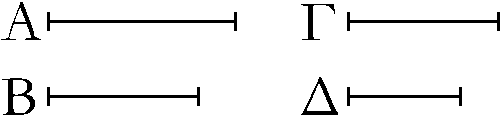
\includegraphics[width=0.8\textwidth]{Book05/fig14g.pdf}}

\gr{Πρῶτον γὰρ τὸ Α πρὸς δεύτερον τὸ Β τὸν αὐτὸν ἐθέτω λόγον καὶ
τρίτον τὸ Γ πρὸς τέταρτον τὸ Δ, μεῖζον δὲ ὸέστω τὸ Α τοῦ Γ; λέγω,
ὅτι καὶ τὸ Β τοῦ Δ μεῖζόν ἐστιν.}

\gr{Ἐπεὶ γὰρ τὸ Α τοῦ Γ μεῖζόν ἐστιν, ὸάλλο δέ, ὃ ὸέτυθεν,
[μέγεθος] τὸ Β, τὸ Α ἄρα πρὸς τὸ Β μείζονα λόγον ἔχει ἢπερ τὸ Γ πρὸς τὸ Β. ὡξ δὲ τὸ Α 	πρὸς τὸ Β, οὁύτως τὸ Γ πρὸς
τὸ
Δ; καὶ τὸ Γ ἄρα πρὸς τὸ Δ μείζονα
λόγον ἔχει ἢπερ τὸ Γ πρὸς τὸ Β. πρὸς ὃ δὲ τὸ αὐτὸ μείζονα
λόγον ἔχει, ἐκεῖνοὸέλασσόν ἐστιν; ὸέλασσον ἄρα τὸ Δ τοῦ Β; ὁώστε
μεῖζόν ἐστι τὸ Β τοῦ Δ.}

\gr{Ὁμοίως δὴ δεῖχομεν, ὅτι κὸὰν ἴσονὸῆ| τὸ Α τῷ Γ,
 ἴσονὸέσται καὶ τὸ Β τῷ Δ, κὸάνὸέλασσονὸῆ| τὸ Α
τοῦ Γ, ὸέλασσονὸέσται καὶ τὸ Β τοῦ Δ.}

\gr{Ἐὰν ἄρα πρῶτον πρὸς δεύτερον τὸν αὐτὸνὸέθῃ λόγον καὶ τρίτον  πρὸς τέταρτον, τὸ δὲ
πρῶτον τοῦ τρίτου μεῖζονὸῆ|, καὶ τὸ δεύτερον τοῦ τετάρτου
μεῖζονὸέσται, κὸὰν ἴσον,  ἴσον, κὸὰνὸέλαττον, ὸέλαττον;
ὅπερ ἔδει δεῖχαι.
}}

\ParallelRText{
\begin{center}
{\large Proposition 14}$^\dag$
\end{center}

If a first (magnitude) has the same ratio to a second  that a third (has) to a fourth, and the first (magnitude) is greater than the third,
(then) the second will also be greater than the fourth. And if (the first magnitude is) equal
(to the third then the second will also be) equal (to the fourth). And
if (the first magnitude is) less (than the third then the second will also be) less (than the fourth).

% Removed epsf size command
\centerline{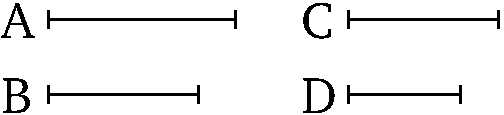
\includegraphics[width=0.8\textwidth]{Book05/fig14e.pdf}}

For let a first (magnitude) $A$ have the same ratio to a second $B$  that a
third $C$ (has) to a fourth $D$. And let $A$ be greater than $C$. I say that $B$
is also greater than $D$.

For since $A$ is greater than $C$, and $B$ (is) another random [magnitude],
$A$ thus has a greater ratio to $B$ than $C$ (has) to $B$ [Prop.~5.8]. And as $A$ (is) to $B$, so $C$ (is) to
$D$. Thus, $C$ also has a greater ratio to $D$ than $C$ (has) to $B$. And that (magnitude) to
which the same (magnitude) has a greater ratio is the lesser
 [Prop.~5.10]. Thus, $D$
(is) less than $B$. Hence, $B$ is greater than $D$.

So, similarly, we can show that even if $A$ is equal to $C$, (then) $B$ will also be equal to $D$, and even if $A$ is less than $C$, (then) $B$ will also be less than $D$.

Thus, if a first (magnitude) has the same ratio to a second  that a third (has) to a fourth, and the first (magnitude) is greater than the third,
(then) the second will also be greater than the fourth. And if (the first magnitude is) equal
(to the third then the second will also be) equal (to the fourth). And
if (the first magnitude  is) less (than the third then the second will also be) less (than the fourth). (Which is) the very thing it was required to show.}
\end{Parallel}
{\footnotesize \noindent$^\dag$ In modern notation, this proposition
reads that if $\alpha:\beta::\gamma:\delta$ then $\alpha \gtreqqless \gamma$ as
$\beta\gtreqqless\delta$.}

%%%%%%
% Prop 5.15
%%%%%%
\pdfbookmark[1]{Proposition 5.15}{pdf5.15}
\begin{Parallel}{}{} 
\ParallelLText{
\begin{center}
{\large \ggn{15}.}
\end{center}\vspace*{-7pt}

\gr{Τὰ μέρη τοῖς ὡσαύτως πολλαπλασίοις τὸν αὐτὸν ἔχει λόγον
ληφθέντα κατάλληλα.}

% Removed epsf size command
\centerline{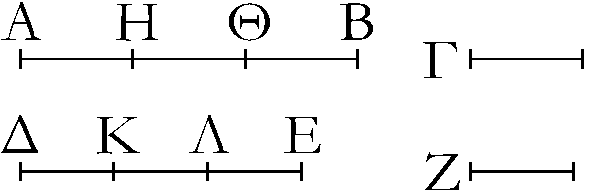
\includegraphics[width=0.8\textwidth]{Book05/fig15g.pdf}}

\gr{Ἔστω γὰρ ἰσάκις πολλαπλάσιον τὸ ΑΒ τοῦ Γ καὶ το ΔΕ τοῦ Ζ;
λέγω, ὅτι ἐστὶν ὡξ τὸ Γ πρὸς τὸ Ζ, οὁύτως τὸ ΑΒ πρὸς τὸ ΔΕ.}

\gr{Ἐπεὶ γὰρ ἰσάκις ἐστὶ πολλαπλάσιον τὸ ΑΒ τοῦ Γ καὶ τὸ ΔΕ τοῦ Ζ,
ὅσα ἄρα ἐστὶν ἐν τῷ ΑΒ μεγέθη ἴσα τῷ Γ, τοσαῦτα καὶ
ἐν τῷ ΔΕ ἴσα τῷ Ζ. διῃρήσθω τὸ μὲν ΑΒ εἰξ τὰ τῷ Γ ἴσα
τὰ ΑΗ, ΗΘ, ΘΒ, τὸ δὲ ΔΕ εἰξ τὰ τῷ Ζ ἴσα τὰ ΔΚ, ΚΛ, ΛΕ;
ὸέσται δὴ  ἴσον τὸ πλῆθος τῶν ΑΗ, ΗΘ, ΘΒ τῷ πλήθει τῶν ΔΚ, ΚΛ, ΛΕ. καὶ ἐπεὶ  ἴσα ἐστὶ τὰ ΑΗ, ΗΘ, ΘΒ  ἀλλήλοις, ὸέστι δὲ καὶ τὰ
ΔΚ, ΚΛ, ΛΕ ἴσα ἀλλήλοις,
ὸέστιν ἄρα
ὡξ τὸ ΑΗ πρὸς τὸ ΔΚ,  οὁύτως τὸ ΗΘ πρὸς τὸ ΚΛ, καὶ τὸ ΘΒ
πρὸς τὸ ΛΕ. ὸέσται ἄρα καὶ ὡξ ὁὲν τῶν ἡγουμένων 
πρὸς ὁὲν τῶν ἑπομένων, οὁύτως ὁάπαντα τὰ ἡγουμένα πρὸς
ὁάπαντα τὰ ἑπόμενα; ὸέστιν ἄρα ὡξ τὸ ΑΗ πρὸς τὸ ΔΚ, οὁύτως
τὸ ΑΒ πρὸς τὸ ΔΕ.  ἴσον δὲ τὸ μὲν ΑΗ τῷ Γ, τὸ δὲ ΔΚ
τῷ Ζ; ὸέστιν ἄρα ὡξ τὸ Γ πρὸς τὸ Ζ οὁύτως τὸ ΑΒ πρὸς 
τὸ ΔΕ.}

\gr{Τὰ  ἄρα μέρη τοῖς ὡσαύτως πολλαπλασίοις τὸν αὐτὸν ἔχει λόγον
ληφθέντα κατάλληλα; ὅπερ ἔδει δεῖχαι.}}

\ParallelRText{
\begin{center}
{\large Proposition 15}$^\dag$
\end{center}

Parts have the same ratio  as similar multiples,
taken in corresponding order.

% Removed epsf size command
\centerline{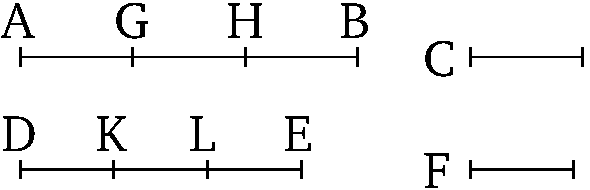
\includegraphics[width=0.8\textwidth]{Book05/fig15e.pdf}}

For let $AB$ and $DE$ be equal multiples of $C$ and $F$ (respectively). I say that
as $C$ is to $F$, so $AB$ (is) to $DE$.

For since $AB$ and $DE$ are equal multiples of $C$ and $F$ (respectively), thus
as many magnitudes as there are in $AB$ equal to $C$, so many (are there) also
in $DE$ equal to $F$. Let $AB$ be divided into (magnitudes) $AG$, $GH$, $HB$, equal to $C$, and $DE$ into (magnitudes) $DK$, $KL$,  $LE$, equal to
$F$. So, the number of (magnitudes) $AG$, $GH$,  $HB$ will equal the number
of (magnitudes) $DK$, $KL$, $LE$.
And since $AG$, $GH$, $HB$ are equal to one another, 
and $DK$, $KL$,  $LE$ are also equal to one another,
thus as $AG$ is to
$DK$, so $GH$ (is) to $KL$, and $HB$ to $LE$ [Prop.~5.7]. And, thus (for proportional magnitudes), as one of the leading
(magnitudes) will be to one of the following, so all of the leading (magnitudes will be)
to all of the following [Prop.~5.12].
Thus, as $AG$ is to $DK$, so $AB$ (is) to $DE$. And $AG$ is equal to $C$, and 
$DK$ to $F$. Thus, as $C$ is to $F$, so $AB$ (is) to $DE$.

Thus, parts have the same ratio  as similar multiples,
taken in corresponding order. (Which is) the very thing it was required to
show.}
\end{Parallel}
{\footnotesize \noindent$^\dag$ In modern notation, this proposition
reads that $\alpha:\beta::m\,\alpha:m\,\beta$.}

%%%%%%
% Prop 5.16
%%%%%%
\pdfbookmark[1]{Proposition 5.16}{pdf5.16}
\begin{Parallel}{}{} 
\ParallelLText{
\begin{center}
{\large \ggn{16}.}
\end{center}\vspace*{-7pt}

\gr{Ἐὰν τέσσαρα μεγέθη ἀνάλογονὸῆ|, καὶ ἐναλλὰχ ἀνάλογονὸέσται.}

\gr{Ἔστω τέσσαρα μεγέθη ἀνάλογον τὰ 
Α, Β, Γ, Δ, ὡξ τὸ Α πρὸς τὸ Β, οὁύτως τὸ Γ πρὸς τὸ Δ; λέγω,
ὅτι καὶ ἐναλλὰχ [ἀνάλογον] ὸέσται, ὡξ τὸ Α πρὸς τὸ Γ, 
οὁύτως τὸ Β πρὸς τὸ Δ.}

\gr{Εἰλήφθω γὰρ τῶν μὲν Α, Β ἰσάκις πολλαπλάσια τὰ Ε, Ζ, τῶν
δὲ Γ, Δὸάλλα, ὁὰ ὸέτυθεν, ἰσάκις πολλαπλάσια τὰ Η, Θ.}\\

% Removed epsf size command
\centerline{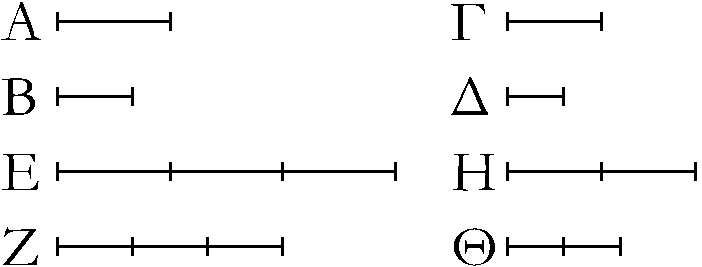
\includegraphics[width=0.8\textwidth]{Book05/fig16g.pdf}}

\gr{Καὶ ἐπεὶ ἰσάκις ἐστὶ πολλαπλάσιον τὸ Ε τοῦ Α καὶ τὸ Ζ τοῦ
Β, τὰ δὲ μέρη τοῖς ὡσαύτως πολλαπλασίοις τὸν αὐτὸν ἔχει
λόγον, ὸέστιν ἄρα ὡξ τὸ Α πρὸς
τὸ Β, οὁύτως τὸ Ε πρὸς τὸ Ζ. ὡξ δὲ τὸ Α πρὸς τὸ Β,
οὁύτως τὸ Γ πρὸς τὸ Δ; καὶ ὡξ ἄρα τὸ Γ πρὸς
τὸ Δ, οὁύτως τὸ Ε πρὸς τὸ Ζ. πάλιν, ἐπεὶ τὰ Η, Θ τῶν Γ, Δ
ἰσάκις ἐστὶ πολλαπλάσια, ὸέστιν ἄρα ὡξ τὸ Γ πρὸς τὸ Δ, οὁύτως
τὸ Η πρὸς τὸ Θ. ὡξ δὲ τὸ Γ πρὸς τὸ Δ, [οὁύτως] τὸ Ε πρὸς
τὸ Ζ; καὶ ὡξ ἄρα τὸ Ε πρὸς τὸ Ζ, οὁύτως τὸ Η πρὸς τὸ Θ. ἒαν
δὲ τέσσαρα μεγέθη ἀνάλογονὸῆ|, τὸ δὲ πρῶτον τοῦ τρίτου
μεῖζονὸῆ|, καὶ τὸ δεύτερον τοῦ τετάρτου μεῖζονὸέσται,
κὸὰν ἴσον,  ἴσον, κὸάνὸέλαττον, ὸέλαττον. εἰ  ἄρα ὑπερέθει
τὸ Ε τοῦ Η, ὑπερέθει καὶ τὸ Ζ τοῦ Θ, καὶ εἰ  ἴσον,  ἴσον,
καὶ εἰ ὸέλαττον, ὸέλαττον. καί ἐστι τὰ μὲν Ε, Ζ τῶν Α, Β
ἰσάκις πολλαπλάσια, τὰ δὲ Η, Θ τῶν Γ, Δὸάλλα, ὁὰ ὸέτυθεν, ἰσάκις
πολλαπλάσια; ὸέστιν ἄρα ὡξ τὸ Α πρὸς τὸ Γ, οὁύτως τὸ Β πρὸς
τὸ Δ.}

\gr{Ἐὰν ἄρα τέσσαρα μεγέθη ἀνάλογονὸῆ|, καὶ ἐναλλὰχ
ἀνάλογονὸέσται; ὅπερ ἔδει δεῖχαι.}}

\ParallelRText{
\begin{center}
{\large Proposition 16}$^\dag$
\end{center}

If four magnitudes are proportional, (then) they will
also be proportional alternately.

Let $A$, $B$, $C$ and $D$ be four proportional magnitudes, (such that) as $A$
(is) to $B$, so $C$ (is) to $D$. I say that they will also be [proportional]
 alternately, (so that) as $A$ (is) to $C$, so $B$ (is) to $D$.
 
For let the equal multiples $E$ and $F$ be taken of $A$ and $B$ (respectively),
and the other random equal multiples $G$ and $H$ of $C$ and $D$ (respectively).

% Removed epsf size command
\centerline{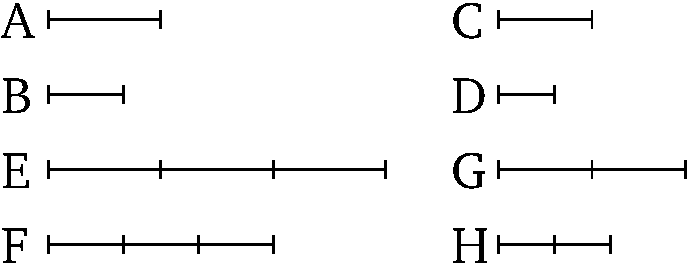
\includegraphics[width=0.8\textwidth]{Book05/fig16e.pdf}}

And since $E$ and $F$ are equal multiples of $A$ and $B$ (respectively),
and parts  have the same ratio as similar multiples [Prop.~5.15], thus as $A$ is to $B$, so $E$ (is) to $F$.
But as $A$ (is) to $B$, so $C$ (is) to $D$. And, thus, as $C$ (is) to $D$, so
$E$ (is) to $F$ [Prop.~5.11].
Again, since $G$ and $H$ are equal multiples of $C$ and $D$ (respectively),  thus
as $C$  is to $D$, so $G$ (is) to $H$ [Prop.~5.15].
But as $C$ (is) to $D$, [so] $E$ (is) to $F$. And, thus, as $E$ (is) to $F$, so
$G$ (is) to $H$ [Prop.~5.11]. And if four magnitudes are proportional, and the first is greater than the third, (then)
the second will also be greater than the fourth, and if (the first is) equal
(to the third then the second will also be) equal (to the fourth), and if
(the first is) less (than the third then the second will also be) less (than the fourth)
[Prop.~5.14]. Thus, if $E$ exceeds $G$ (then)
$F$ also exceeds $H$, and if ($E$ is) equal (to $G$ then $F$ is also) equal (to $H$), and if
($E$ is) less (than $G$ then $F$ is also) less (than $H$). And $E$ and $F$ are equal multiples of $A$ and $B$ (respectively), and $G$ and $H$ other random equal multiples
of $C$ and $D$ (respectively). Thus, as $A$ is to $C$, so $B$ (is) to $D$ [Def.~5.5].

Thus, if four magnitudes are proportional, (then) they will
also be proportional  alternately. (Which is) the very thing it was required to show.}
\end{Parallel}
{\footnotesize \noindent$^\dag$ In modern notation, this proposition
reads that if $\alpha:\beta::\gamma:\delta$ then $\alpha:\gamma::\beta:\delta$.}

%%%%%%
% Prop 5.17
%%%%%%
\pdfbookmark[1]{Proposition 5.17}{pdf5.17}
\begin{Parallel}{}{} 
\ParallelLText{
\begin{center}
{\large \ggn{17}.}
\end{center}\vspace*{-7pt}

\gr{Ἐὰν συγκείμενα μεγέθη ἀνάλογονὸῆ|, καὶ διαιρεθέντα ἀνάλογονὸέσται.}

% Removed epsf size command
\centerline{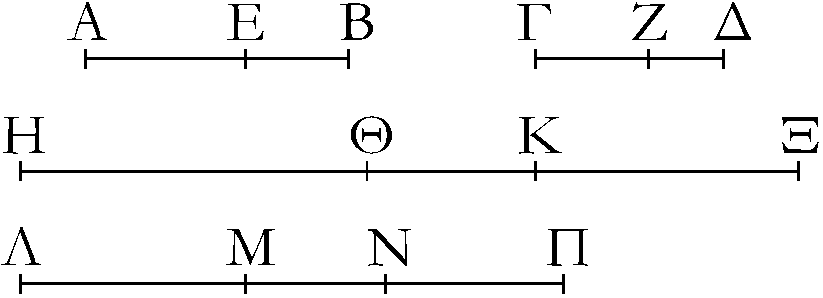
\includegraphics[width=0.8\textwidth]{Book05/fig17g.pdf}}

\gr{Ἔστω συγκείμενα μεγέθη ἀνάλογον τὰ ΑΒ, ΒΕ, ΓΔ, ΔΖ, ὡξ τὸ ΑΒ
πρὸς τὸ ΒΕ, οὁύτως τὸ ΓΔ πρὸς τὸ ΔΖ; λέγω, ὅτι καὶ διαιρεθέντα
ἀνάλογονὸέσται, ὡξ τὸ ΑΕ πρὸς τὸ ΕΒ, οὁύτως τὸ ΓΖ πρὸς τὸ ΔΖ.}

\gr{Εἰλήφθω γὰρ τῶν μὲν ΑΕ, ΕΒ, ΓΖ, ΖΔ ἰσάκις πολλαπλάσια τὰ ΗΘ,
ΘΚ, ΛΜ, ΜΝ, τῶν δὲ ΕΒ, ΖΔὸάλλα, ὁὰ ὸέτυθεν, ἰσάκις
πολλαπλάσια τὰ ΚΧ, ΝΠ.}

\gr{Καὶ ἐπεὶ ἰσάκις ἐστὶ πολλαπλάσιον τὸ ΗΘ τοῦ ΑΕ καὶ τὸ ΘΚ
τοῦ ΕΒ, ἰσάκις ἄρα ἐστὶ πολλαπλάσιον τὸ ΗΘ τοῦ ΑΕ καὶ τὸ ΗΚ
τοῦ ΑΒ. ἰσάκις δέ ἐστι πολλαπλάσιον τὸ ΗΘ τοῦ ΑΕ καὶ τὸ ΛΜ
τοῦ ΓΖ; ἰσάκις ἄρα ἐστὶ πολλαπλάσιον τὸ ΗΚ τοῦ ΑΒ καὶ τὸ ΛΜ
τοῦ ΓΖ. πάλιν, ἐπεὶ ἰσάκις ἐστὶ πολλαπλάσιον τὸ ΛΜ τοῦ ΓΖ
καὶ τὸ ΜΝ τοῦ ΖΔ, ἰσάκις ἄρα ἐστὶ πολλαπλάσιον τὸ ΛΜ τοῦ ΓΖ
καὶ τὸ ΛΝ τοῦ ΓΔ. ἰσάκις δὲ ὸῆν πολλαπλάσιον τὸ ΛΜ τοῦ ΓΖ καὶ τὸ
ΗΚ τοῦ ΑΒ; ἰσάκις ἄρα ἐστὶ πολλαπλάσιον τὸ ΗΚ τοῦ ΑΒ καὶ τὸ ΛΝ
τοῦ ΓΔ. τὰ ΗΚ, ΛΝ ἄρα τῶν ΑΒ, ΓΔ ἰσάκις ἐστὶ πολλαπλάσια.
πάλιν, ἐπεὶ ἰσάκις ἐστὶ πολλαπλασίον τὸ ΘΚ τοῦ ΕΒ
καὶ τὸ ΜΝ τοῦ ΖΔ, ὸέστι δὲ καὶ τὸ ΚΧ τοῦ ΕΒ ἰσάκις πολλαπλάσιον
καὶ τὸ ΝΠ τοῦ ΖΔ, καὶ συντεθὲν τὸ ΘΧ τοῦ ΕΒ ἰσάκις ἐστὶ
πολλαπλάσιον καὶ τὸ ΜΠ τοῦ ΖΔ. 
καὶ ἐπεί ἐστιν ὡξ τὸ ΑΒ πρὸς  τὸ ΒΕ, οὁύτως τὸ ΓΔ πρὸς τὸ ΔΖ, καὶ εὸίληπται τῶν μὲν ΑΒ, ΓΔ ἰσάκις πολλαπλάσια τὰ
ΗΚ, ΛΝ, τῶν δὲ ΕΒ, ΖΔ ἰσάκις πολλαπλάσια τὰ ΘΧ, ΜΠ, εἰ  ἄρα
ὑπερέθει τὸ ΗΚ τοῦ ΘΧ, ὑπερέθει καὶ τὸ ΛΝ τοῦ ΜΠ, καὶ εἰ
 ἴσον,  ἴσον, καὶ εἰ ὸέλαττον, ὸέλαττον. ὑπερεθέτω δὴ τὸ ΗΚ τοῦ
ΘΧ, καὶ κοινοῦ ἀφαιρεθέντος τοῦ ΘΚ ὑπερέθει ἄρα καὶ τὸ
ΗΘ τοῦ ΚΧ. ἀλλα εἰ ὑπερεῖθε
τὸ ΗΚ τοῦ ΘΧ
ὑπερεῖθε καὶ τὸ ΛΝ τοῦ ΜΠ; ὑπερέθει ἄρα καὶ τὸ ΛΝ τοῦ ΜΠ,
καὶ κοινοῦ ἀφαιρεθέντος τοῦ ΜΝ ὑπερέθει
καὶ τὸ ΛΜ τοῦ ΝΠ; ὁώστε εἰ ὑπερέθει τὸ ΗΘ τοῦ ΚΧ,
ὑπερέθει καὶ τὸ ΛΜ τοῦ  ΝΠ. ὁμοίως δὴ δεῖχομεν, ὅτι κὸὰν ἴσονὸῆ| τὸ ΗΘ τῷ ΚΧ,  ἴσονὸέσται καὶ τὸ ΛΜ τῷ ΝΠ, κὸὰνὸέλαττον, ὸέλαττον. καί ἐστι τὰ μὲν ΗΘ, ΛΜ τῶν ΑΕ, ΓΖ
ἰσάκις πολλαπλάσια, τὰ δὲ ΚΧ, ΝΠ τῶν ΕΒ, ΖΔὸάλλα, ὁὰ ὸέτυθεν,
ἰσάκις πολλαπλάσια; ὸέστιν ἄρα ὡξ τὸ ΑΕ πρὸς τὸ ΕΒ, οὁύτως τὸ
ΓΖ πρὸς τὸ ΖΔ.}

\gr{Ἐὰν ἄρα συγκείμενα μεγέθη ἀνάλογονὸῆ|, καὶ διαιρεθέντα ἀνάλογονὸέσται; ὅπερ ἔδει δεῖχαι.}}

\ParallelRText{
\begin{center}
{\large Proposition 17}$^\dag$
\end{center}

If composed  magnitudes are proportional, (then) they will also be proportional (when)
separarted.

% Removed epsf size command
\centerline{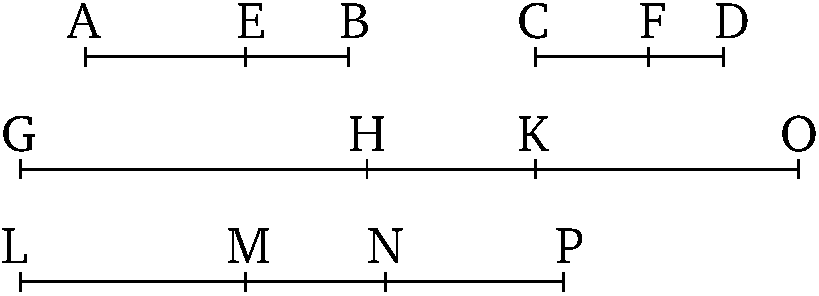
\includegraphics[width=0.8\textwidth]{Book05/fig17e.pdf}}

Let $AB$, $BE$, $CD$, and $DF$ be composed magnitudes (which are) proportional,
(so that) as $AB$ (is) to $BE$, so $CD$ (is) to $DF$. I say that they will also be
proportional (when) separated, (so that) as $AE$ (is) to $EB$, so  $CF$ (is)
to $DF$.

For let the equal multiples $GH$, $HK$, $LM$, and $MN$ be taken of
$AE$, $EB$, $CF$, and $FD$ (respectively), and the other random equal multiples
$KO$ and $NP$ of $EB$ and $FD$ (respectively).

And since $GH$ and $HK$ are equal multiples of $AE$ and $EB$ (respectively), 
$GH$ and $GK$ are thus equal multiples of $AE$ and $AB$ (respectively) [Prop.~5.1]. But $GH$ and $LM$ are equal
multiples of $AE$ and $CF$ (respectively). Thus, $GK$ and $LM$ are equal
multiples of $AB$ and $CF$ (respectively). Again, since $LM$ and $MN$ are equal
multiples of $CF$ and $FD$ (respectively), $LM$ and $LN$ are thus equal multiples
of $CF$ and $CD$ (respectively) [Prop.~5.1]. 
And $LM$ and $GK$ were equal multiples of $CF$ and $AB$ (respectively).
Thus, $GK$ and $LN$ are equal multiples of $AB$ and $CD$ (respectively).
Thus, $GK$, $LN$ are equal multiples of $AB$, $CD$. Again, since
$HK$ and $MN$ are equal multiples of $EB$ and $FD$ (respectively), and $KO$
and $NP$ are also  equal multiples of $EB$ and $FD$ (respectively),  (then), added together, $HO$ and $MP$ are also equal multiples of $EB$ and $FD$ (respectively) [Prop.~5.2]. And since as $AB$ (is) to $BE$, so
$CD$ (is) to $DF$, and the equal multiples $GK$, $LN$ be
taken of $AB$, $CD$, and the equal multiples $HO$, $MP$ of $EB$, $FD$, thus 
if $GK$ exceeds $HO$ (then) $LN$ also exceeds $MP$, and if ($GK$ is) equal
(to $HO$ then $LN$ is also) equal (to $MP$), and if ($GK$ is) less (than $HO$ then
$LN$ is also) less (than $MP$) [Def.~5.5]. So let $GK$ exceed $HO$, and thus, $HK$ being taken away from
both, $GH$ exceeds $KO$. But (we saw that) if $GK$ was exceeding $HO$ (then)
$LN$ was also exceeding $MP$. Thus, $LN$ also exceeds $MP$, and, $MN$ being
taken away from both, $LM$ also exceeds $NP$.  Hence, if $GH$ exceeds $KO$
(then) $LM$ also exceeds $NP$. So, similarly, we can show that even if
$GH$ is equal to $KO$ (then) $LM$ will also be equal to $NP$, and
even if ($GH$ is) less (than $KO$ then $LM$ will also be) less (than $NP$).
And $GH$, $LM$ are equal multiples of $AE$, $CF$, and $KO$, $NP$ other random
equal multiples of $EB$, $FD$. Thus, as $AE$ is to $EB$, so  $CF$ (is) to $FD$ [Def.~5.5].

Thus, if composed magnitudes are proportional, (then) they will also be proportional (when)
separarted. (Which is) the very thing it was required to show.}
\end{Parallel}
{\footnotesize \noindent$^\dag$ In modern notation, this proposition
reads that if $\alpha+\beta:\beta::\gamma+\delta:\delta$ then $\alpha:\beta::
\gamma:\delta$.}

%%%%%%
% Prop 5.18
%%%%%%
\pdfbookmark[1]{Proposition 5.18}{pdf5.18}
\begin{Parallel}{}{} 
\ParallelLText{
\begin{center}
{\large \ggn{18}.}
\end{center}\vspace*{-7pt}

\gr{Ἐὰν διῃρημένα μεγέθη ἀνάλογονὸῆ|, καὶ συντεθέντα ἀνάλογονὸέσται.}

% Removed epsf size command
\centerline{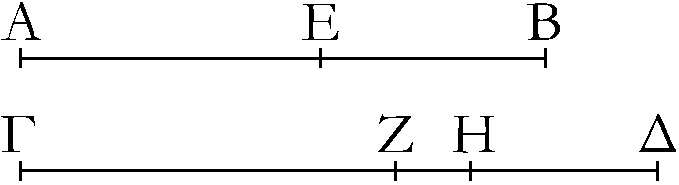
\includegraphics[width=0.8\textwidth]{Book05/fig18g.pdf}}

\gr{Ἔστω διῃρημένα μεγέθη ἀνάλογον τὰ ΑΕ, ΕΒ, ΓΖ, ΖΔ, ὡξ τὸ ΑΕ
πρὸς τὸ ΕΒ, οὁύτως τὸ ΓΖ πρὸς τὸ ΖΔ; λέγω, ὅτι καὶ συντεθέντα
ἀνάλογονὸέσται, ὡξ τὸ ΑΒ πρὸς τὸ ΒΕ, οὁύτως τὸ ΓΔ πρὸς τὸ ΖΔ.}

\gr{Εἰ γὰρ μή ἐστὶν ὡξ τὸ ΑΒ πρὸς τὸ ΒΕ, οὁύτως τὸ ΓΔ πρὸς
τὸ ΔΖ, ὸέσται ὡξ τὸ ΑΒ πρὸς τὸ ΒΕ, οὁύτως τὸ ΓΔ ἢτοι πρὸςὸέλασσόν τι τοῦ ΔΖὸὴ πρὸς μεῖζον.}

\gr{Ἔστω πρότερον πρὸςὸέλασσον τὸ ΔΗ. καὶ ἐπεί ἐστιν ὡξ τὸ ΑΒ
πρὸς τὸ ΒΕ, οὁύτως τὸ ΓΔ πρὸς τὸ ΔΗ,  συγκείμενα μεγέθη ἀνάλογόν
ἐστιν; ὁώστε καὶ διαιρεθέντα ἀνάλογονὸέσται. ὸέστιν ἄρα ὡξ τὸ ΑΕ
πρὸς τὸ ΕΒ, οὁύτως τὸ ΓΗ πρὸς τὸ ΗΔ. ὑπόκειται δὲ καὶ ὡξ τὸ
ΑΕ πρὸς τὸ ΕΒ, οὁύτως τὸ ΓΖ πρὸς τὸ ΖΔ. καὶ ὡξ ἄρα τὸ ΓΗ πρὸς
τὸ ΗΔ, οὁύτως τὸ ΓΖ πρὸς τὸ ΖΔ. μεῖζον δὲ τὸ πρῶτον τὸ ΓΗ τοῦ
τρίτου τοῦ ΓΖ; μεῖζον ἄρα καὶ τὸ δεύτερον
τὸ ΗΔ τοῦ τετάρτου τοῦ ΖΔ. ἀλλὰ καὶ ὸέλαττον; ὅπερ
ἐστὶν ἀδύνατον; οὐκ ἄρα ἐστὶν ὡξ τὸ ΑΒ πρὸς τὸ ΒΕ, οὁύτως
τὸ ΓΔ πρὸςὸέλασσον
 τοῦ ΖΔ. ὁμοίως δὴ δείχομεν, ὅτι
οὐδὲ πρὸς μεῖζον; πρὸς αὐτὸ  ἄρα.}

\gr{ Ἐὰν ἄρα διῃρημένα μεγέθη ἀνάλογονὸῆ|, καὶ συντεθέντα ἀνάλογονὸέσται; ὅπερ ἔδει δεῖχαι.}}

\ParallelRText{
\begin{center}
{\large Proposition 18}$^\dag$
\end{center}

If separated  magnitudes are proportional,  (then) they will also be proportional (when)
composed.

% Removed epsf size command
\centerline{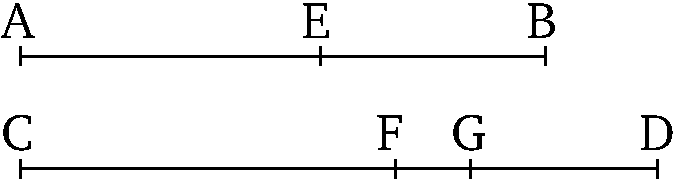
\includegraphics[width=0.8\textwidth]{Book05/fig18e.pdf}}

Let $AE$, $EB$, $CF$, and $FD$ be separated magnitudes (which are) proportional,
(so that) as $AE$ (is) to $EB$, so  $CF$ (is) to $FD$. I say that they will also be proportional (when)  composed, (so that) as $AB$ (is) to $BE$, so  $CD$ (is) to $FD$.

For if (it is) not (the case that) as $AB$ is to $BE$, so $CD$ (is) to $FD$, (then) it will
surely be (the case that) as $AB$ (is) to $BE$, so
 $CD$ is either to some (magnitude) less than $DF$, or (some magnitude) greater (than $DF$).$^\ddag$
 
 Let it, first of all, be to (some magnitude) less (than $DF$), (namely) $DG$. And since composed magnitudes are proportional, (so that) as $AB$ is
 to $BE$, so $CD$ (is) to $DG$,  they will  thus also be proportional (when) separated 
 [Prop.~5.17]. Thus, as $AE$ is to $EB$, so
 $CG$ (is) to $GD$. But it was also assumed that as $AE$ (is) to $EB$, so $CF$ (is)
 to $FD$. Thus, (it is) also (the case that) as $CG$ (is) to $GD$, so $CF$ (is) to $FD$ [Prop.~5.11]. And the first (magnitude) $CG$ (is)
 greater than the third $CF$. Thus, the second (magnitude) $GD$ (is)
 also greater than the fourth $FD$ [Prop.~5.14]. 
 But (it is) also less. The very thing is impossible. Thus, (it is) not (the case that) as $AB$ is to $BE$, so $CD$ (is) to less than $FD$. Similarly, we can show
 that neither (is it the case) to greater (than $FD$). Thus, (it is the case) to
 the same (as $FD$).
 
 Thus, if separated  magnitudes are proportional,  (then) they will also be 
 proportional (when)
composed. (Which is) the very thing it was required to show.}
\end{Parallel}
{\footnotesize \noindent$^\dag$ In modern notation, this proposition
reads that if $\alpha:\beta::\gamma:\delta$ then $\alpha+\beta:\beta::
\gamma+\delta:\delta$.}\\
{\footnotesize \noindent$^\ddag$ Here, Euclid assumes, without proof, that
a fourth magnitude proportional to three given magnitudes can always
be found.}

%%%%%%
% Prop 5.19
%%%%%%
\pdfbookmark[1]{Proposition 5.19}{pdf5.19}
\begin{Parallel}{}{} 
\ParallelLText{
\begin{center}
{\large \ggn{19}.}
\end{center}\vspace*{-7pt}

\gr{Ἐὰνὸῆ| ὡξ ὅλον πρὸς ὅλον, οὁύτως ἀφαιρεθὲν πρὸς
ἀφαιρεθέν, καὶ τὸ λοιπὸν πρὸς τὸ λοιπὸνὸέσται ὡξ ὅλον
πρὸς ὅλον.}\\

% Removed epsf size command
\centerline{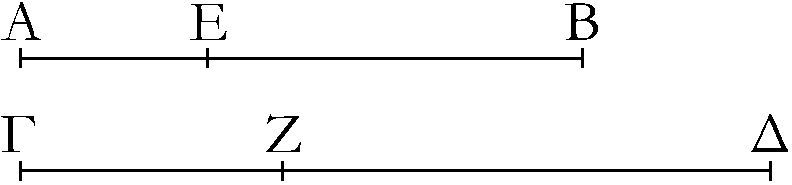
\includegraphics[width=0.8\textwidth]{Book05/fig19g.pdf}}

\gr{Ἔστω γὰρ ὡξ ὅλον τὸ ΑΒ πρὸς ὅλον τὸ ΓΔ, οὁύτως ἀφαιρεθὲν
τὸ ΑΕ πρὸς ἀφαιρεθὲν τὸ ΓΖ; λέγω, ὅτι καὶ λοιπὸν τὸ ΕΒ πρὸς
λοιπὸν τὸ ΖΔὸέσται ὡξ ὅλον τὸ ΑΒ πρὸς ὅλον τὸ ΓΔ.}

\gr{Ἐπεὶ γάρ ἐστιν ὡξ τὸ ΑΒ πρὸς τὸ ΓΔ, οὁύτως τὸ ΑΕ πρὸς τὸ
ΓΖ, καὶ ἐναλλὰχ ὡξ τὸ ΒΑ πρὸς τὸ ΑΕ, οὁύτως τὸ ΔΓ πρὸς τὸ ΓΖ.
καὶ ἐπεὶ συγκείμενα μεγέθη ἀνάλογόν ἐστιν, καὶ διαιρεθέντα
ἀνάλογονὸέσται, ὡξ τὸ ΒΕ πρὸς τὸ ΕΑ, οὁύτως τὸ ΔΖ πρὸς
τὸ ΓΖ; καὶ ἐναλλάχ, ὡξ τὸ ΒΕ πρὸς τὸ ΔΖ, οὁύτως τὸ ΕΑ πρὸς
τὸ ΖΓ. ὡξ δὲ τὸ ΑΕ πρὸς τὸ ΓΖ,  οὁύτως ὑπόκειται ὅλον τὸ ΑΒ πρὸς ὅλον
τὸ ΓΔ. καὶ λοιπὸν ἄρα τὸ ΕΒ πρὸς λοιπὸν τὸ ΖΔὸέσται ὡξ ὅλον
τὸ ΑΒ πρὸς ὅλον τὸ ΓΔ.}

\gr{Ἐὰν ἄραὸῆ| ὡξ ὅλον πρὸς ὅλον, οὁύτως ἀφαιρεθὲν πρὸς
ἀφαιρεθέν, καὶ τὸ λοιπὸν πρὸς τὸ λοιπὸνὸέσται ὡξ ὅλον
πρὸς ὅλον [ὅπερ ἔδει δεῖχαι].}

\gr{ {[}Ka`i >epe`i >ede'iqjh <wc t`o AB pr`oc t`o GD, o<'utwc t`o EB
pr`oc t`o ZD, ka`i >enall`ax <wc t`o AB pr`oc t`o BE o<'utwc t`o
GD pr`oc t`o ZD, sugke'imena >'ara meg'ejh >an'alog'on >estin;
>ede'iqjh d`e <wc t`o BA pr`oc t`o AE, o<'utwc t`o DG pr`oc t`o GZ;
ka'i >estin >anastr'eyanti].}\\~\\

\begin{center}
{\large \gr{Πόρισμα}.}
\end{center}\vspace*{-7pt}

\gr{Ἐκ δὴ τούτου φανερόν, ὅτι ἒαν συγκείμενα μεγέθη
ἀνάλογονὸῆ|, καὶ ἀναστρέψαντι ἀνάλογονὸέσται; ὅπερ ἔδει
δεῖχαι.}}

\ParallelRText{
\begin{center}
{\large Proposition 19}$^\dag$
\end{center}

If as the whole is to the whole so the (part) taken
away is to the (part) taken away, (then) the remainder to the remainder will
also be as the whole (is) to the whole.

% Removed epsf size command
\centerline{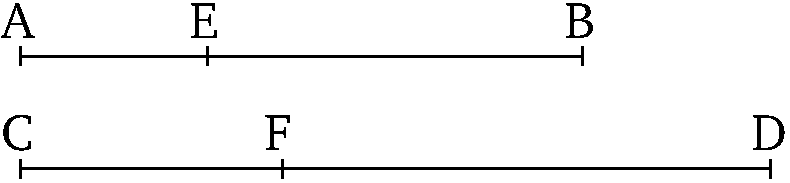
\includegraphics[width=0.8\textwidth]{Book05/fig19e.pdf}}

For let the whole $AB$ be to the whole $CD$ as the (part) taken away $AE$
(is) to the (part) taken away $CF$. I say that the remainder $EB$
to the remainder $FD$ will also be as the whole $AB$ (is) to the whole $CD$.

For since as $AB$ is to $CD$, so $AE$ (is) to $CF$, (it is) also (the case), alternately, 
(that) as $BA$ (is)
to $AE$, so $DC$ (is) to $CF$ [Prop.~5.16].
And since composed magnitudes are proportional, (then) they will also
be proportional (when) separated, (so that) as $BE$ (is) to $EA$, so $DF$ (is)
to $CF$ [Prop.~5.17].
Also, alternately, as $BE$ (is) to $DF$, so $EA$ (is) to $FC$ [Prop.~5.16]. And it was assumed that as
$AE$ (is) to $CF$, so the whole $AB$ (is) to the whole $CD$. And, thus,  as the
remainder $EB$ (is) to the remainder $FD$, so the whole $AB$ will be to the
whole $CD$.

Thus, if as the whole is to the whole so the (part) taken
away is to the (part) taken away, (then) the remainder to the remainder will
also be as the whole (is) to the whole. [(Which is) the very thing it was required to show.]

\mbox{[}And since it was shown (that) as $AB$ (is) to $CD$, so $EB$ (is) to $FD$, (it is)
also (the case), alternately, (that) as $AB$ (is) to $BE$, so $CD$ (is) to $FD$. 
Thus, composed magnitudes are proportional. And it was shown
(that) as $BA$ (is) to $AE$, so $DC$ (is) to $CF$. And (the latter) is converted (from the former).]\\

\begin{center}
{\large Corollary}$^\ddag$
\end{center}\vspace*{-7pt}

So (it is) clear, from this, that if composed magnitudes are proportional,
 (then) they will also be proportional (when) converted.
(Which is) the very thing it was required to show.}
\end{Parallel}
{\footnotesize \noindent$^\dag$ In modern notation, this proposition
reads that if $\alpha:\beta::\gamma:\delta$ then
$\alpha:\beta::\alpha-\gamma:\beta-\delta$.\\[0.5ex]
$^\ddag$ In modern notation, this corollary reads
that if $\alpha:\beta::\gamma:\delta$ then $\alpha:\alpha-\beta::\gamma:\gamma-\delta$.}

%%%%%%
% Prop 5.20
%%%%%%
\pdfbookmark[1]{Proposition 5.20}{pdf5.20}
\begin{Parallel}{}{} 
\ParallelLText{
\begin{center}
{\large \ggn{20}.}
\end{center}\vspace*{-7pt}

\gr{Ἐὰνὸῆ| τρία μεγέθη καὶ ὸάλλα αὐτοῖς ἴσα τὸ
πλῆθος, σύνδυο λαμβανόμενα καὶ ἐν τῷ αὐτῷ
λόγω, διὸ ὸίσου δὲ τὸ πρῶτον τοῦ τρίτου μεῖζονὸῆ|, καὶ τὸ τέταρτον τοῦ ὁέκτου μεῖζονὸέσται,
κὸὰν ἴσον,  ἴσον, κὸὰνὸέλαττον, ὸέλαττον.}\\~\\~\\

% Removed epsf size command
\centerline{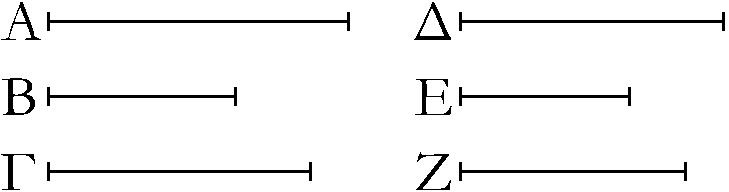
\includegraphics[width=0.8\textwidth]{Book05/fig20g.pdf}}

\gr{Ἔστω τρία μεγέθη τὰ Α, Β, Γ, καὶ ὸάλλα αὐτοῖς ἴσα τὸ πλῆθος τὰ Δ, Ε, Ζ, σύνδυο λαμβανόμενα
ἐν τῷ αὐτῷ λόγῳ, ὡξ μὲν τὸ Α πρὸς τὸ Β,
οὁύτως τὸ Δ πρὸς τὸ Ε, ὡξ δὲ τὸ Β πρὸς τὸ Γ,
οὁύτως τὸ Ε πρὸς τὸ Ζ, διὸ ὸίσου δὲ μεῖζονὸέστω
τὸ Α τοῦ Γ;
 λέγω,
ὅτι καὶ τὸ Δ τοῦ Ζ μεῖζονὸέσται, κὸὰν ἴσον,  ἴσον,
κὸὰνὸέλαττον, ὸέλαττον.}

\gr{Ἐπεὶ γὰρ μεῖζόν ἐστι τὸ Α τοῦ Γ, ὸάλλο δέ τι τὸ
Β, τὸ δὲ μεῖζον πρὸς τὸ αὐτὸ μείζονα λόγον ἔχει ἢπερ τὸ ὸέλαττον, τὸ Α ἄρα πρὸς τὸ Β μείζονα λόγον ἔχει ἢπερ τὸ Γ πρὸς τὸ Β. ἀλλὸ ὡξ μὲν τὸ Α πρὸς τὸ Β
[οὁύτως] τὸ Δ πρὸς τὸ Ε, ὡξ δὲ τὸ Γ πρὸς τὸ Β, ἀνάπαλιν
οὁύτως τὸ Ζ πρὸς τὸ Ε; καὶ τὸ Δ ἄρα πρὸς τὸ Ε μείζονα λόγον ἔχει ἢπερ τὸ Ζ πρὸς τὸ Ε. τῶν δὲ πρὸς τὸ αὐτὸ λόγον ἐθόντων
τὸ μείζονα λόγον ἔχον μεῖζόν ἐστιν. μεῖζον ἄρα τὸ Δ τοῦ Ζ.
ὁμοίως δὴ δείχομεν, ὅτι κὸὰν ἴσονὸῆ| τὸ Α τῷ Γ,  ἴσονὸέσται καὶ τὸ Δ τῷ Ζ, κὸὰνὸέλαττον, ὸέλαττον.}

\gr{Ἐὰν ἄραὸῆ| τρία μεγέθη καὶ ὸάλλα αὐτοῖς ἴσα τὸ
πλῆθος, σύνδυο λαμβανόμενα καὶ ἐν τῷ αὐτῷ
λόγω, διὸ ὸίσου δὲ τὸ πρῶτον τοῦ τρίτου μεῖζονὸῆ|, καὶ τὸ τέταρτον τοῦ ὁέκτου μεῖζονὸέσται,
κὸὰν ἴσον,  ἴσον, κὸὰνὸέλαττον, ὸέλαττον; ὅπερ ἔδει
δεῖχαι.}}

\ParallelRText{
\begin{center}
{\large Proposition 20}$^\dag$
\end{center}

If there are three magnitudes, and others of equal
 number to them,   (being) also in the same ratio taken two by two, and (if),
via equality,  the first is greater
than the third (then) the fourth will also be greater than the sixth. And
 if (the first is) equal (to the third then the fourth will also be) equal
(to the sixth). 
And if (the first is) less (than the third then the fourth will also be) less (than
the sixth).

% Removed epsf size command
\centerline{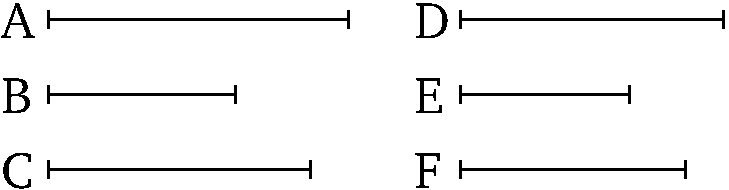
\includegraphics[width=0.8\textwidth]{Book05/fig20e.pdf}}

Let $A$, $B$, and $C$ be three magnitudes, and $D$, $E$, $F$ other (magnitudes) of equal
number to them, (being) in the same ratio taken two by two, (so that)
as $A$ (is) to $B$, so $D$ (is) to $E$, and as $B$ (is) to $C$, so $E$ (is) to $F$. And let $A$
be greater than $C$, via equality. I say that $D$ will also be greater
than $F$. And if ($A$ is) equal (to $C$ then $D$ will also be) equal (to $F$). And
if ($A$ is) less (than $C$ then $D$ will also be) less (than $F$).

For since $A$ is greater than $C$, and $B$ some other (magnitude), and
the greater (magnitude) has a greater ratio than the lesser to the same (magnitude) [Prop.~5.8], $A$ thus has
a greater ratio to $B$ than $C$ (has) to $B$. But as $A$ (is) to $B$, [so] $D$ (is)
to $E$. And, inversely, as $C$ (is) to $B$,  so  $F$ (is) to $E$ [Prop.~5.7~corr.]. Thus, $D$ also has a greater
ratio to $E$ than $F$ (has) to $E$ [Prop.~5.13]. And for (magnitudes) having a ratio to the
same (magnitude), that having the greater ratio is greater [Prop.~5.10]. Thus, $D$ (is) greater than $F$.
Similarly, we can show that even if $A$ is equal to $C$ (then) $D$ will also
be equal to $F$, and even if ($A$ is) less (than $C$ then $D$ will also
be) less (than $F$).

Thus, if there are three magnitudes, and others of equal
number to them,   (being) also in the same ratio taken two by two, and (if),
via equality, the first is greater
than the third, (then) the fourth will also be greater than the sixth. And
 if (the first is) equal (to the third then the fourth will also be) equal
(to the sixth). And (if the first is) less (than the third then the fourth will also be) less (than
the sixth). (Which is) the very thing it was required to show.}
\end{Parallel}
{\footnotesize \noindent$^\dag$ In modern notation, this proposition
reads that if $\alpha:\beta::\delta:\epsilon$ and $\beta:\gamma::\epsilon:\zeta$ then $\alpha\gtreqqless\gamma$ as $\delta\gtreqqless\zeta$.}

%%%%%%
% Prop 5.21
%%%%%%
\pdfbookmark[1]{Proposition 5.21}{pdf5.21}
\begin{Parallel}{}{} 
\ParallelLText{
\begin{center}
{\large \ggn{21}.}
\end{center}\vspace*{-7pt}

\gr{Ἐὰνὸῆ| τρία μεγέθη καὶ ὸάλλα αὐτοῖς ἴσα τὸ πλῆθος σύνδυο λαμβανόμενα καὶ ἐν τῷ αὐτῷ λόγῳ, ὸῆ| δὲ τεταραγμένη αὐτῶν
ἡ ἀναλογία, διὸ ὸίσου δὲ τὸ πρῶτον τοῦ τρίτου μεῖζονὸῆ|, καὶ
τὸ τέταρτον τοῦ ὁέκτου μεῖζονὸέσται, κὸὰν ἴσον,  ἴσον, κὸὰνὸέλαττον, ὸέλαττον.}\\~\\~\\

% Removed epsf size command
\centerline{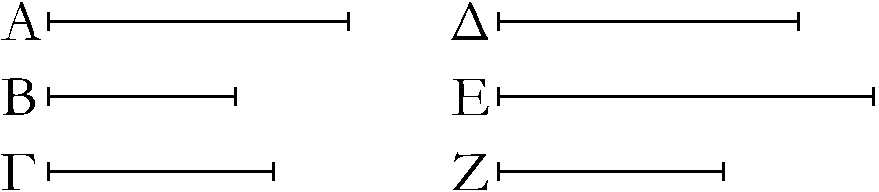
\includegraphics[width=0.8\textwidth]{Book05/fig21g.pdf}}

\gr{Ἔστω τρία μεγέθη τὰ Α, Β, Γ καὶ ὸάλλα αὐτοῖς ἴσα τὸ πλῆθος
τὰ Δ, Ε, Ζ, σύνδυο λαμβανόμενα καὶ ἐν τῷ αὐτῷ λόγῳ, ὸέστω δὲ
τεταραγμένη αὐτῶν ἡ ἀναλογία, ὡξ μὲν τὸ Α πρὸς τὸ Β, οὁύτως
τὸ Ε πρὸς τὸ Ζ, ὡξ δὲ τὸ Β πρὸς τὸ Γ, οὁύτως τὸ Δ πρὸς τὸ Ε,
διὸ ὸίσου δὲ τὸ Α τοῦ Γ μεῖζονὸέστω; λέγω, ὅτι
καὶ τὸ Δ τοῦ Ζ μεῖζονὸέσται, κὸὰν ἴσον,  ἴσον, κὸὰνὸὲλαττον,
ὸὲλαττον.}

\gr{Ἐπεὶ γὰρ μεῖζόν ἐστι τὸ Α τοῦ Γ, ὸάλλο δέ τι τὸ Β, τὸ Α ἄρα
πρὸς τὸ Β μείζονα λόγον ἔχει ἢπερ τὸ Γ πρὸς τὸ Β. ἀλλὸ ὡξ
μὲν τὸ Α πρὸς τὸ Β, οὁύτως τὸ Ε πρὸς τὸ Ζ, ὡξ δὲ τὸ Γ πρὸς
τὸ Β, ἀνάπαλιν οὁύτως τὸ Ε πρὸς τὸ Δ. καὶ τὸ Ε ἄρα πρὸς τὸ Ζ
μείζονα λόγον ἔχει ἢπερ τὸ Ε πρὸς τὸ Δ. πρὸς ὃ δὲ τὸ αὐτὸ μείζονα λόγον ἔχει, ἐκεῖνοὸέλασσόν ἐστιν; ὸέλασσον ἄρα
ἐστὶ τὸ Ζ τοῦ Δ; μεῖζον ἄρα ἐστὶ τὸ Δ τοῦ Ζ.
ὁμοίως δὴ δείχομεν, ὅτι κὸὰν ἴσονὸῆ|
τὸ Α τῷ Γ,  ἴσονὸέσται καὶ τὸ Δ τῷ Ζ, κὸὰνὸέλαττον, ὸέλαττον.}

\gr{Ἐὰν ἄραὸῆ| τρία μεγέθη καὶ ὸάλλα αὐτοῖς ἴσα τὸ πλῆθος, σύνδυο λαμβανόμενα καὶ ἐν τῷ αὐτῷ λόγῳ, ὸῆ| δὲ τεταραγμένη αὐτῶν
ἡ ἀναλογία, διὸ ὸίσου δὲ τὸ πρῶτον τοῦ τρίτου μεῖζονὸῆ|, καὶ
τὸ τέταρτον τοῦ ὁέκτου μεῖζονὸέσται, κὸὰν ἴσον,  ἴσον, κὸὰνὸέλαττον, ὸέλαττον; ὅπερ ἔδει δεῖχαι.}}

\ParallelRText{
\begin{center}
{\large Proposition 21}$^\dag$
\end{center}

If there are three magnitudes, and others of equal
 number to them, (being) also in the same ratio taken two by two, and (if)
their proportion (is) perturbed, and (if), via equality,
the first is greater than the third (then) the fourth will also
be greater than the sixth. And if (the first is) equal (to the third then the
fourth will also be) equal (to the sixth).
And if (the first is) less (than the third then the fourth will also be) less (than
the sixth).

% Removed epsf size command
\centerline{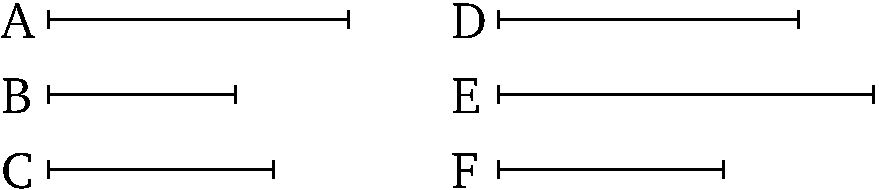
\includegraphics[width=0.8\textwidth]{Book05/fig21e.pdf}}

Let $A$, $B$, and $C$ be three magnitudes, and $D$, $E$, $F$ other (magnitudes)
of equal number to them, (being) in the same ratio taken two by two. And let their proportion be perturbed, (so that) as $A$ (is) to $B$, so $E$ (is) to $F$, and as
$B$ (is) to $C$, so $D$ (is) to $E$. And let $A$  be greater than $C$, via equality. I
say that $D$ will also be greater than $F$.
 And if ($A$ is) equal (to $C$ then $D$ will also be) equal (to $F$). And
if ($A$ is) less (than $C$ then $D$ will also be) less (than $F$).

For since $A$ is greater than $C$, and $B$ some other (magnitude),  $A$ thus
has a greater ratio to $B$ than $C$ (has) to $B$ [Prop.~5.8]. But as $A$ (is) to $B$,
so $E$ (is) to $F$. And, inversely, as $C$ (is) to $B$, so $E$ (is) to $D$ [Prop.~5.7~corr.]. Thus, $E$ also has a greater
ratio to $F$ than $E$ (has) to $D$ [Prop.~5.13]. And that (magnitude) to which the same (magnitude)  has a greater ratio  is (the) lesser (magnitude) [Prop.~5.10].
Thus, $F$ is less than $D$. Thus, $D$ is greater than $F$. Similarly, we can show that
even if $A$ is equal to $C$ (then) $D$ will also
be equal to $F$, and even if ($A$ is) less (than $C$ then $D$ will also
be) less (than $F$).

Thus, if there are three magnitudes, and others of equal
 number to them, (being) also in the same ratio taken two by two, and (if)
their proportion (is) perturbed, and (if), via equality,
the first is greater than the third (then) the fourth will also
be greater than the sixth. And if (the first is) equal (to the third then the fourth
will also be) equal (to the sixth).
And if (the first is) less (than the third then the fourth will also be) less (than
the sixth). (Which is) the very thing it was required to show.}
\end{Parallel}
{\footnotesize \noindent$^\dag$ In modern notation, this proposition
reads that if $\alpha:\beta::\epsilon:\zeta$ and $\beta:\gamma::\delta:\epsilon$ then $\alpha\gtreqqless\gamma$ as $\delta\gtreqqless\zeta$.}

%%%%%%
% Prop 5.22
%%%%%%
\pdfbookmark[1]{Proposition 5.22}{pdf5.22}
\begin{Parallel}{}{} 
\ParallelLText{
\begin{center}
{\large \ggn{22}.}
\end{center}\vspace*{-7pt}

\gr{Ἐὰνὸῆ| ὁποσαοῦν μεγέθη καὶ ὸάλλα αὐτοῖς ἴσα τὸ πλῆθος,
σύνδυο λαμβανόμενα καὶ ἐν τῷ αὐτῷ λόγῳ, καὶ διὸ ὸίσου
ἐν τῷ αὐτῷ λόγῳ ὸέσται.}\\

% Removed epsf size command
\centerline{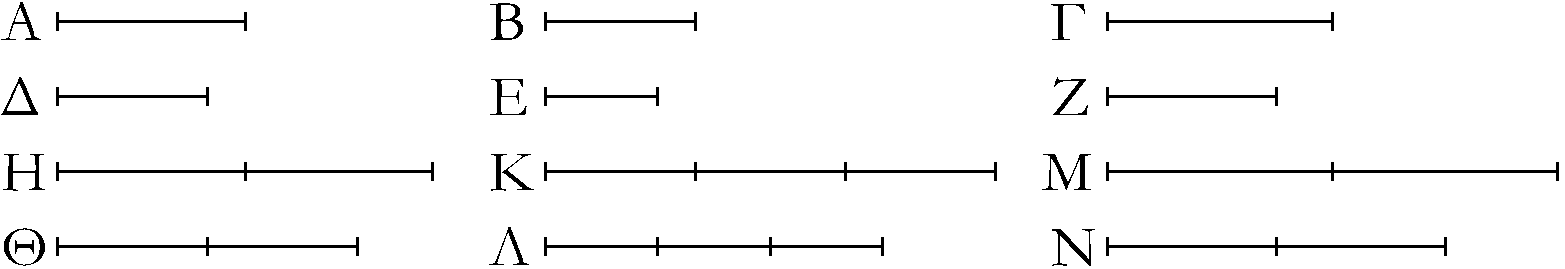
\includegraphics[width=0.8\textwidth]{Book05/fig22g.pdf}}

\gr{Ἔστω ὁποσαοῦν μεγέθη τὰ Α, Β, Γ καὶ ὸάλλα αὐτοῖς ἴσα τὸ
πλῆθος τὰ Δ, Ε, Ζ, σύνδυο λαμβανόμενα ἐν τῷ αὐτῷ λόγῳ,
ὡξ μὲν τὸ Α πρὸς τὸ Β, οὁύτως τὸ Δ πρὸς τὸ Ε, ὡξ δὲ
τὸ Β πρὸς τὸ Γ, οὁύτως τὸ Ε πρὸς τὸ Ζ; λέγω, ὅτι
καὶ διὸ ὸίσου ἐν τῷ αὐτῳ λόγῳ
ὸέσται.}

\gr{Εἰλήφθω γὰρ τῶν μὲν Α, Δ ἰσάκις πολλαπλάσια
τὰ Η, Θ, τῶν δὲ Β, Εὸάλλα, ὁὰ ὸέτυθεν, ἰσάκις πολλαπλάσια
τὰ Κ, Λ, καὶ ὸέτι τῶν Γ, Ζὸάλλα, ὁὰ ὸέτυθεν, ἰσάκις πολλαπλάσια
τὰ Μ, Ν.}

\gr{Καὶ ἐπεί  ἐστιν ὡξ τὸ Α πρὸς τὸ Β, οὁύτως τὸ Δ πρὸς τὸ Ε,
καὶ εὸίληπται τῶν μὲν Α, Δ ἰσάκις πολλαπλάσια τὰ
Η, Θ, τῶν δὲ Β, Εὸάλλα, ὁὰ ὸέτυθεν, ἰσάκις πολλαπλάσια
τὰ Κ, Λ, ὸέστιν ἄρα ὡξ τὸ Η πρὸς τὸ Κ, οὁύτως τὸ Θ πρὸς τὸ Λ.
δὶα τὰ αὐτὰ δὴ καὶ ὡξ τὸ Κ πρὸς τὸ Μ, οὁύτως τὸ
Λ πρὸς
τὸ Ν. ἐπεὶ οὸῦν τρία μεγέθη ἐστὶ τὰ Η, Κ, Μ, καὶ ὸάλλα
αὐτοῖς ἴσα
τὸ πλῆθος τὰ Θ, Λ, Ν, σύνδυο λαμβανόμενα καὶ ἐν τῷ αὐτῷ
λόγῳ, διὸ ὸίσου ἄρα, εἰ ὑπερέθει τὸ Η τοῦ Μ,
ὑπερέθει καὶ τὸ Θ τοῦ Ν, καὶ εἰ  ἴσον,  ἴσον, καὶ
εἰ ὸέλαττον, ὸέλαττον. καί ἐστι τὰ μὲν Η, Θ τῶν Α, Δ
ἰσάκις πολλαπλάσια, τὰ δὲ Μ, Ν τῶν Γ, Ζὸάλλα, ὁὰ
ὸέτυθεν, ἰσάκις πολλαπλάσια. ὸέστιν ἄρα ὡξ τὸ Α πρὸς
τὸ Γ, οὁύτως τὸ Δ πρὸς τὸ Ζ.}

\gr{Ἐὰν ἄραὸῆ| ὁποσαοῦν μεγέθη καὶ ὸάλλα αὐτοῖς ἴσα τὸ πλῆθος,
σύνδυο λαμβανόμενα ἐν τῷ αὐτῷ λόγῳ, καὶ διὸ ὸίσου
ἐν τῷ αὐτῷ λόγῳ ὸέσται; ὅπερ ἔδει δεῖχαι.}}

\ParallelRText{
\begin{center}
{\large Proposition 22}$^\dag$
\end{center}

If there are any number of magnitudes
whatsoever, and (some) other (magnitudes)  of equal  number to them, (which are)
also in the same ratio taken two by two, (then) they will also be in the
same ratio via equality.

% Removed epsf size command
\centerline{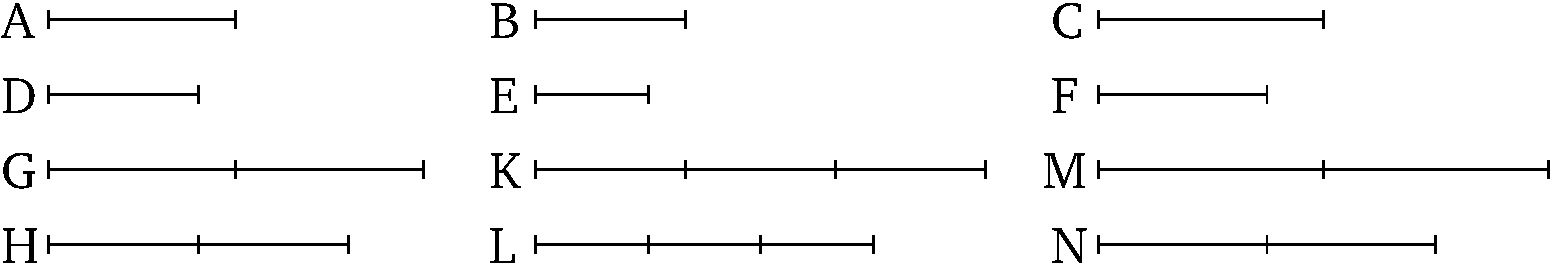
\includegraphics[width=0.8\textwidth]{Book05/fig22e.pdf}}

Let there be any number of magnitudes whatsoever, $A$, $B$,  $C$, and
(some) other (magnitudes), $D$, $E$, $F$, of equal number to them, (which are)
in the same ratio taken two by two, (so that) as $A$ (is) to $B$, so
$D$ (is) to $E$, and as $B$ (is) to $C$, so $E$ (is) to $F$. I say that they
will also be in the same ratio via equality. (That is, as $A$ is to $C$, so
$D$ is to $F$.)

For let the equal multiples $G$ and $H$ be taken of $A$ and $D$ (respectively), and the other random equal multiples $K$ and $L$ of $B$ and
$E$ (respectively), and the yet other random equal multiples $M$ and $N$ of
$C$ and $F$ (respectively).

And since as $A$ is to $B$, so $D$ (is) to $E$, and the equal multiples $G$ and $H$
have been taken of $A$ and $D$ (respectively), and the other random
equal multiples $K$ and $L$ of $B$ and $E$ (respectively), thus as $G$ is to $K$,
so $H$ (is) to $L$ [Prop.~5.4]. And, so, for the same
(reasons), as $K$ (is) to $M$, so $L$ (is) to $N$. Therefore, since $G$, $K$, and $M$ are three magnitudes, and $H$, $L$, and $N$ other (magnitudes) of equal number to them,
(which are) also in the same ratio taken two by two, thus, via equality,
if $G$ exceeds $M$ (then) $H$ also exceeds $N$, and if ($G$ is) equal (to $M$ then $H$
is also) equal (to $N$), and if ($G$ is) less (than $M$ then $H$
is also) less (than $N$) [Prop.~5.20].
And  $G$ and $H$ are equal multiples of $A$ and $D$ (respectively),
and $M$ and $N$ other random equal multiples of $C$ and $F$ (respectively).
Thus, as $A$ is to $C$, so $D$ (is) to $F$ [Def.~5.5].

Thus, if there are any number of magnitudes
whatsoever, and (some) other (magnitudes) of equal number to them, (which are)
also in the same ratio taken two by two, (then) they will also be in the
same ratio via equality. (Which is) the very thing
it was required to show.}
\end{Parallel}
{\footnotesize \noindent $^\dag$ In modern notation, this proposition
reads that if $\alpha:\beta::\epsilon:\zeta$ and $\beta:\gamma::\zeta:\eta$ 
and $\gamma:\delta::\eta:\theta$ 
then $\alpha:\delta::\epsilon:\theta$.}

%%%%%%
% Prop 5.23
%%%%%%
\pdfbookmark[1]{Proposition 5.23}{pdf5.23}
\begin{Parallel}{}{} 
\ParallelLText{
\begin{center}
{\large\ggn{23}.}
\end{center}\vspace*{-7pt}

\gr{Ἐὰνὸῆ| τρία μεγέθη καὶ ὸάλλα αὐτοῖς ἴσα τὸ πλῆθος σύνδυο
λαμβανόμενα ἐν τῷ αὐτῷ λόγῳ, ὸῆ| δὲ τεταραγμένη αὐτῶν
ἡ ἀναλογία, καὶ διὸ ὸίσου ἐν τῷ αὐτῷ λόγῳ ὸέσται.}\\

% Removed epsf size command
\centerline{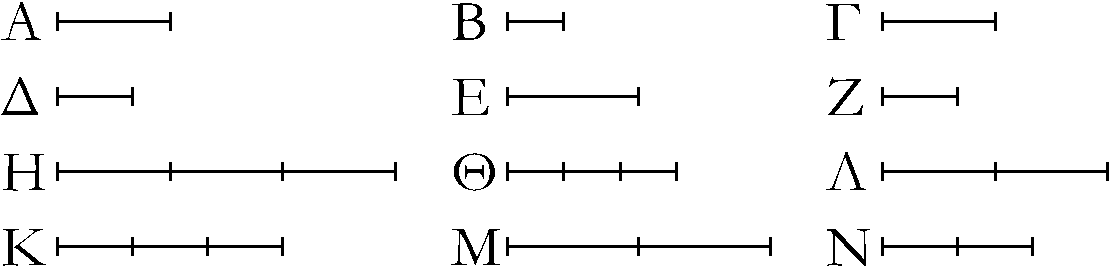
\includegraphics[width=0.8\textwidth]{Book05/fig23g.pdf}}

\gr{Ἔστω τρία μεγέθη τὰ Α, Β, Γ καὶ ὸάλλα αὐτοῖς ἴσα τὸ πλῆθος 
σύνδυο λαμβανόμενα ἐν τῷ αὐτῷ λόγῳ τὰ Δ, Ε, Ζ, ὸέστω
δὲ τεταραγμένη αὐτῶν ἡ ἀναλογία, ὡξ μὲν τὸ Α πρὸς τὸ Β,
οὁύτως τὸ Ε πρὸς τὸ Ζ, ὡξ δὲ τὸ Β πρὸς τὸ Γ, οὁύτως τὸ Δ
πρὸς τὸ Ε; λέγω, ὅτι ἐστὶν ὡξ τὸ Α πρὸς τὸ Γ, οὁύτως
τὸ Δ πρὸς τὸ Ζ.}

\gr{Εἰλήφθω τῶν μὲν Α, Β, Δ ἰσάκις πολλαπλάσια τὰ Η, Θ, Κ, τῶν
δὲ Γ, Ε, Ζὸάλλα, ὁὰ ὸέτυθεν, ἰσάκις πολλαπλάσια τὰ Λ, Μ, Ν.}

\gr{Καὶ ἐπεὶ ἰσάκις ἐστὶ πολλαπλάσια τὰ Η, Θ τῶν Α, Β, τὰ δὲ μέρη
τοὶξ ὡσαύτως πολλαπλασίοις τὸν αὐτὸν ἔχει λόγον,
ὸέστιν ἄρα ὡξ τὸ Α πρὸς τὸ Β, οὁύτως τὸ Η πρὸς
τὸ Θ. διὰ τὰ αὐτὰ δὴ καὶ ὡξ τὸ Ε πρὸς τὸ Ζ, οὁύτως τὸ Μ
πρὸς τὸ Ν; καί ἐστιν ὡξ τὸ Α πρὸς τὸ Β, οὁύτως τὸ Ε πρὸς
τὸ Ζ; καὶ ὡξ ἄρα τὸ Η πρὸς τὸ Θ, οὁύτως τὸ Μ πρὸς τὸ Ν.
καὶ ἐπεί ἐστιν ὡξ τὸ Β πρὸς τὸ Γ, οὁύτως τὸ Δ πρὸς τὸ Ε,
καὶ ἐναλλὰχ ὡξ τὸ Β πρὸς τὸ Δ, οὁύτως τὸ Γ πρὸς τὸ Ε. καὶ
ἐπεὶ τὰ Θ, Κ τῶν Β, Δ ἰσάκις ἐστὶ πολλαπλάσια, τὰ δὲ μέρη 
τοῖς ἰσάκις πολλαπλασίοις τὸν αὐτὸν ἔχει λόγον, ὸέστιν ἄρα
ὡξ τὸ Β πρὸς τὸ Δ, οὁύτως τὸ Θ πρὸς τὸ Κ. ἀλλὸ ὡξ 
τὸ Β πρὸς τὸ Δ, οὁύτως τὸ Γ πρὸς τὸ Ε; καὶ ὡξ ἄρα τὸ Θ πρὸς
τὸ Κ, οὁύτως τὸ Γ πρὸς τὸ Ε.
 πάλιν, ἐπεὶ τὰ Λ, Μ
τῶν Γ, Ε ἰσάκις ἐστι πολλαπλάσια, ὸέστιν ἄρα ὡξ τὸ Γ
πρὸς τὸ Ε, οὁύτως τὸ Λ πρὸς τὸ Μ. ἀλλὸ ὡξ τὸ Γ πρὸς τὸ Ε,
οὁύτως τὸ Θ πρὸς τὸ Κ; καὶ ὡξ ἄρα τὸ Θ πρὸς τὸ Κ, οὁύτως
τὸ Λ πρὸς τὸ Μ, καὶ ἐναλλὰχ ὡξ τὸ Θ πρὸς τὸ Λ, τὸ Κ
πρὸς τὸ Μ. ἐδείθθη δὲ καὶ ὡξ τὸ Η πρὸς τὸ Θ, οὁύτως
τὸ Μ πρὸς τὸ Ν. ἐπεὶ οὸῦν τρία μεγέθη ἐστὶ τὰ Η, Θ, Λ,
καὶ ὸάλλα αὐτοις ἴσα τὸ πλῆθος τὰ Κ, Μ, Ν σύνδυο λαμβανόμενα
ἐν τῷ αὐτῷ λόγῳ, καί ἐστιν αὐτῶν τεταραγμένη ἡ
ἀναλογία, διὸ ὸίσου ἄρα, εἰ ὑπερέθει τὸ Η
τοῦ Λ, ὑπερέθει καὶ τὸ Κ τοῦ Ν, καὶ εἰ  ἴσον,  ἴσον, καὶ
εἰ ὸέλαττον, ὸέλαττον. καί ἐστι τὰ μὲν Η, Κ τῶν Α, Δ ἰσάκις
πολλαπλάσια, τὰ δὲ Λ, Ν τῶν Γ, Ζ. ὸέστιν ἄρα ὡξ τὸ Α πρὸς
τὸ Γ, οὁύτως τὸ Δ πρὸς τὸ Ζ.}

\gr{Ἐὰν ἄραὸῆ| τρία μεγέθη καὶ ὸάλλα αὐτοῖς ἴσα τὸ πλῆθος σύνδυο
λαμβανόμενα ἐν τῷ αὐτῷ λόγῳ, ὸῆ| δὲ τεταραγμένη αὐτῶν
ἡ ἀναλογία, καὶ διὸ ὸίσου ἐν τῷ αὐτῷ λόγῳ ὸέσται;
ὅπερ ἔδει δεῖχαι.}}

\ParallelRText{
\begin{center}
{\large Proposition 23}$^\dag$
\end{center}

If there are three magnitudes, and others of equal number to them, (being) in the same ratio taken two by two, and (if) their
proportion is perturbed, (then) they will also be in the same ratio via equality.

% Removed epsf size command
\centerline{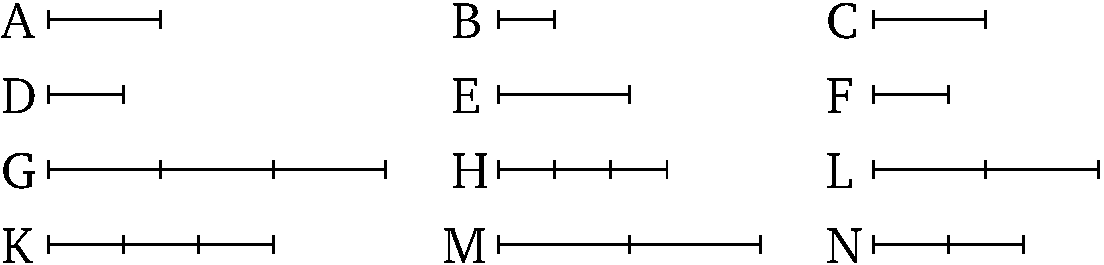
\includegraphics[width=0.8\textwidth]{Book05/fig23e.pdf}}

Let $A$, $B$, and $C$ be three magnitudes, and $D$, $E$ and $F$ other (magnitudes) of equal  number to them, (being) in the same ratio taken two by two.
And let their proportion be perturbed, (so that) as $A$ (is) to $B$, so $E$ (is) to $F$,
and as $B$ (is) to $C$, so $D$ (is) to $E$. I say that as $A$ is to $C$, so $D$ (is) to $F$.

Let the equal multiples $G$, $H$, and $K$ be taken of $A$, $B$, and $D$ (respectively), and the other random equal multiples $L$, $M$, and $N$ of
$C$, $E$, and $F$ (respectively).

And since $G$ and $H$ are equal multiples of $A$ and $B$ (respectively), and
parts have the same ratio as similar multiples [Prop.~5.15], thus as $A$ (is) to $B$, so $G$ (is) to $H$. 
And, so, for the same (reasons), as $E$ (is) to $F$, so $M$ (is) to $N$. And as
$A$ is to $B$, so $E$ (is) to $F$.  And, thus, as $G$ (is) to $H$, so $M$ (is) to $N$ [Prop.~5.11]. And since as $B$ is to $C$, so $D$ (is) to $E$,
also, alternately, as $B$ (is) to $D$, so $C$ (is) to $E$ [Prop.~5.16]. And since $H$ and $K$ are equal multiples
of $B$ and $D$ (respectively), and parts have the same ratio as similar multiples
[Prop.~5.15], thus as $B$ is to $D$, so $H$
(is) to $K$. But, as $B$ (is) to $D$, so $C$ (is) to $E$.  And, thus, as $H$ (is) to $K$, so $C$ (is) to $E$ [Prop.~5.11]. Again, since
$L$ and $M$ are  equal multiples of $C$ and $E$ (respectively), thus as
$C$ is to $E$, so $L$ (is) to $M$ [Prop.~5.15].
But, as $C$ (is) to $E$, so $H$ (is) to $K$. And, thus, as $H$ (is) to $K$,
so $L$ (is) to $M$ [Prop.~5.11]. Also, alternately,
as $H$ (is) to $L$, so $K$ (is) to $M$ [Prop.~5.16].
And it was also shown (that) as $G$ (is) to $H$, so $M$ (is) to $N$. Therefore,
since $G$, $H$, and $L$ are three magnitudes, and $K$, $M$, and $N$ other (magnitudes)
of equal number to them, (being) in the same ratio taken two by two, 
and their proportion is perturbed, thus, via equality, if $G$ exceeds
$L$ (then) $K$ also exceeds $N$, and if ($G$ is) equal (to $L$ then $K$ is also) equal (to $N$),
and if ($G$ is) less (than $L$ then $K$ is also) less (than $N$)  [Prop.~5.21]. And $G$ and $K$ are equal
multiples of $A$ and $D$ (respectively), and $L$ and $N$ of $C$ and $F$ (respectively). 
Thus, as $A$ (is) to $C$, so $D$ (is) to $F$  [Def.~5.5].

Thus, if there are three magnitudes, and others of  equal number to them, (being) in the same ratio taken two by two, and (if) their
proportion is perturbed, (then) they will also be in the same ratio via equality.
(Which is) the very thing it was required to show.}
\end{Parallel}
{\footnotesize \noindent$^\dag$ In modern notation, this proposition
reads that if $\alpha:\beta::\epsilon:\zeta$ and $\beta:\gamma::\delta:\epsilon$ then $\alpha:\gamma::\delta:\zeta$.}

%%%%%%
% Prop 5.24
%%%%%%
\pdfbookmark[1]{Proposition 5.24}{pdf5.24}
\begin{Parallel}{}{} 
\ParallelLText{
\begin{center}
{\large \ggn{24}.}
\end{center}\vspace*{-7pt}

\gr{Ἐὰν πρῶτον πρὸς δεύτερον τὸν αὐτὸνὸέθῃ λόγον καὶ τρίτον
πρὸς τέταρτον, ὸέθῃ δὲ καὶ πέμπτον πρὸς δεύτερον τὸν αὐτὸν
λόγον καὶ ὁέκτον πρὸς τέταρτον, καὶ συντεθὲν πρῶτον καὶ
πέμπτον πρὸς δεύτερον τὸν αὐτὸν ὁέχει λόγον καὶ τρίτον
καὶ ὁέκτον πρὸς τέταρτον.}

\gr{Πρῶτον γὰρ τὸ ΑΒ πρὸς δεύρερον τὸ Γ τὸν αὐτὸν ἐθέτω
λόγον καὶ τρίτον τὸ ΔΕ πρὸς τέταρτον τὸ Ζ, ἐθέτω δὲ καὶ πέμπτον
τὸ ΒΗ πρὸς δεύτερον τὸ Γ τὸν αὐτὸν λόγον καὶ ὁέκτον τὸ ΕΘ
πρὸς τέταρτον τὸ Ζ; λέγω, ὅτι καὶ συντεθὲν πρῶτον καὶ πέμπτον
τὸ ΑΗ πρὸς δεύτερον τὸ Γ τὸν αὐτὸν ὁέχει λόγον, καὶ
τρίτον καὶ ὁέκτον τὸ ΔΘ πρὸς τέταρτον τὸ Ζ.}\\~\\

% Removed epsf size command
\centerline{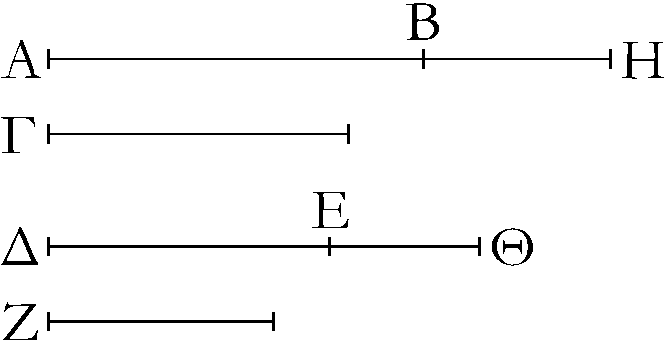
\includegraphics[width=0.8\textwidth]{Book05/fig24g.pdf}}

\gr{Ἐπεὶ γάρ ἐστιν ὡξ τὸ ΒΗ πρὸς τὸ Γ, οὁύτως τὸ ΕΘ πρὸς τὸ Ζ,
ἀνάπαλιν ἄρα ὡξ τὸ Γ πρὸς τὸ ΒΗ, οὁύτως
τὸ Ζ πρὸς τὸ ΕΘ. ἐπεὶ οὸῦν ἐστιν ὡξ τὸ ΑΒ πρὸς τὸ Γ,
οὁύτως τὸ ΔΕ πρὸς τὸ Ζ, ὡξ δὲ τὸ Γ πρὸς τὸ ΒΗ, οὁύτως
τὸ Ζ πρὸς τὸ ΕΘ, διὸ ὸίσου ἄρα ἐστὶν ὡξ τὸ ΑΒ πρὸς τὸ ΒΗ, οὁύτως
τὸ ΔΕ πρὸς τὸ ΕΘ. καὶ ἐπεὶ διῃρημένα μεγέθη ἀνάλογόν ἐστιν,
καὶ συντεθέντα ἀνάλογονὸέσται; ὸέστιν ἄρα ὡξ τὸ ΑΗ πρὸς τὸ ΗΒ,
οὁύτως τὸ ΔΘ πρὸς τὸ ΘΕ. ὸέστι δὲ καὶ ὡξ τὸ ΒΗ πρὸς τὸ Γ, οὁύτως
τὸ ΕΘ πρὸς τὸ Ζ;
διὸ ὸίσου ἄρα ἐστὶν ὡξ τὸ ΑΗ πρὸς τὸ Γ, οὁύτως τὸ
ΔΘ πρὸς τὸ Ζ.}

\gr{Ἐὰν ἄρα πρῶτον πρὸς δεύτερον τὸν αὐτὸνὸέθῃ λόγον καὶ τρίτον
πρὸς τέταρτον, ὸέθῃ δὲ καὶ πέμπτον πρὸς δεύτερον τὸν αὐτὸν
λόγον καὶ ὁέκτον πρὸς τέταρτον, καὶ συντεθὲν πρῶτον καὶ
πέμπτον πρὸς δεύτερον τὸν αὐτὸν ὁέχει λόγον καὶ τρίτον
καὶ ὁέκτον πρὸς τέταρτον; ὅπερ ἔδει δεὶχαι.}}

\ParallelRText{
\begin{center}
{\large Proposition 24}$^\dag$
\end{center}

If a first (magnitude) has to a second the same
ratio  that third (has) to a fourth, and a fifth (magnitude)
also has to the second the same ratio that a sixth  (has) to the fourth, (then)
  the first (magnitude) and the fifth, added together, will also have the same ratio to the
 second
 that the third (magnitude) and sixth  (added together, have) to the fourth.
 
 For let a first (magnitude) $AB$ have the same ratio to a second $C$
 that a third $DE$ (has) to a fourth $F$. And let a fifth (magnitude) $BG$
 also have the same ratio to the second $C$ that a sixth $EH$ (has) to
 the fourth $F$. I say that the first (magnitude) and the fifth, added together, $AG$, will also  have the same ratio to the second $C$ that the third (magnitude) and the sixth, (added together), $DH$,  (has) to the fourth $F$.
 
% Removed epsf size command
\centerline{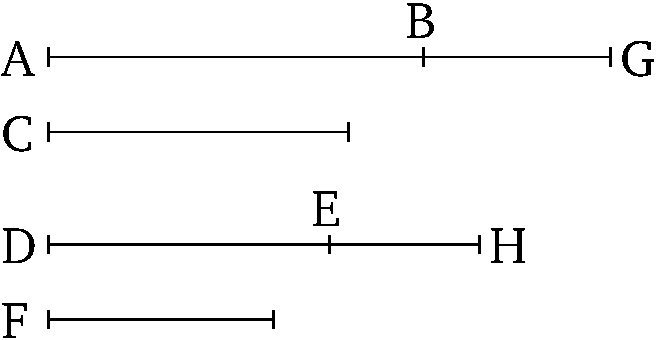
\includegraphics[width=0.8\textwidth]{Book05/fig24e.pdf}}

 For since as $BG$ is to $C$, so $EH$ (is) to $F$,  thus, inversely, as $C$ (is) to $BG$,
 so $F$ (is) to $EH$  [Prop.~5.7~corr.]. Therefore,
 since as $AB$ is to $C$, so $DE$ (is) to $F$, and as $C$ (is) to $BG$, so
 $F$ (is) to $EH$, thus, via equality, as $AB$ is to $BG$, so $DE$ (is) to $EH$ 
[Prop.~5.22]. And since separated magnitudes
are proportional, (then) they will also be proportional (when) composed [Prop.~5.18]. Thus, as $AG$ is to $GB$, so $DH$
(is) to $HE$. And, also, as $BG$ is to $C$, so $EH$ (is) to $F$. Thus, via equality, 
as $AG$ is to $C$, so $DH$ (is) to $F$ [Prop.~5.22].

Thus, if a first (magnitude) has to a second the same
ratio that a third (has) to a fourth, and a fifth (magnitude)
also has to the second the same ratio that a sixth  (has) to the fourth, (then)
the first (magnitude) and the fifth, added together, will also have the same ratio to the
 second
 that the third (magnitude) and the sixth  (added together, have) to the fourth. (Which is) the very thing it was required to show.}
\end{Parallel}
{\footnotesize \noindent$^\dag$ In modern notation, this proposition
reads that if $\alpha:\beta::\gamma:\delta$ and $\epsilon:\beta::\zeta:\delta$ then $\alpha+\epsilon:\beta::\gamma+\zeta:\delta$.}

%%%%%%
% Prop 5.25
%%%%%%
\pdfbookmark[1]{Proposition 5.25}{pdf5.25}
\begin{Parallel}{}{} 
\ParallelLText{
\begin{center}
{\large \ggn{25}.}
\end{center}\vspace*{-7pt}

\gr{Ἐὰν τέσσαρα μεγέθη ἀνάλογονὸῆ|, τὸ μέγιστον [αὐτῶν] καὶ
τὸ ἐλάθιστον δύο τῶν λοιπῶν μείζονά ἐστιν.}\\

% Removed epsf size command
\centerline{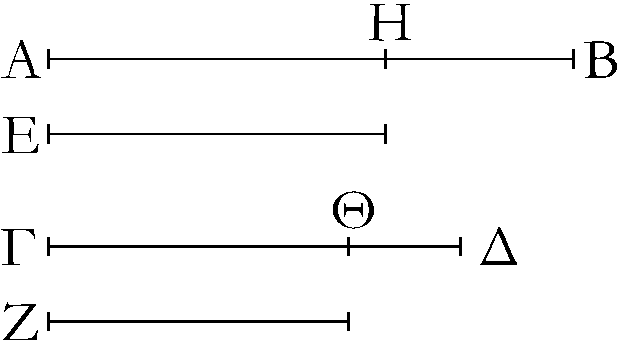
\includegraphics[width=0.8\textwidth]{Book05/fig25g.pdf}}

\gr{Ἔστω τέσσαρα μεγέθη ἀνάλογον τὰ ΑΒ, ΓΔ, Ε, Ζ, ὡξ τὸ ΑΒ
πρὸς τὸ ΓΔ, οὁύτως τὸ Ε πρὸς τὸ Ζ, ὸέστω δὲ μέγιστον μὲν
αὐτῶν τὸ ΑΒ, ἐλάθιστον δὲ τὸ Ζ; λέγω, ὅτι τὰ ΑΒ, Ζ τῶν
ΓΔ, Ε μείζονά ἐστιν.}

\gr{Κείσθω γὰρ τῷ μὲν Ε ἴσον τὸ ΑΗ, τῷ δὲ Ζ ἴσον τὸ ΓΘ.}

\gr{Ἐπεὶ [οὸῦν] ἐστιν ὡξ τὸ ΑΒ πρὸς τὸ ΓΔ, οὁύτως
τὸ Ε πρὸς τὸ Ζ,  ἴσον δὲ τὸ  μὲν Ε τῷ ΑΗ, τὸ δὲ Ζ τῷ ΓΘ,
ὸέστιν ἄρα ὡξ τὸ ΑΒ πρὸς τὸ ΓΔ, οὁύτως
τὸ ΑΗ πρὸς τὸ ΓΘ. καὶ ἐπεί ἐστιν ὡξ ὅλον τὸ ΑΒ πρὸς
ὅλον τὸ ΓΔ, οὁύτως ἀφαιρεθὲν τὸ ΑΗ πρὸς ἀφαιρεθὲν τὸ ΓΘ,
καὶ λοιπὸν ἄρα τὸ ΗΒ πρὸς λοιπὸν τὸ ΘΔὸέσται ὡξ ὅλον
τὸ ΑΒ πρὸς ὅλον τὸ ΓΔ. μεῖζον δὲ τὸ ΑΒ τοῦ ΓΔ; μεῖζον ἄρα καὶ τὸ ΗΒ τοῦ ΘΔ. καὶ ἐπεὶ  ἴσον ἐστὶ τὸ μὲν ΑΗ τῷ
Ε, τὸ δὲ ΓΘ τῷ Ζ, τὰ  ἄρα ΑΗ, Ζ ἴσα ἐστὶ τοῖς
ΓΘ, Ε.
καὶ [ἐπεὶ] ἒαν [ἀνίσοις ἴσα προστεθῆ|, τὰ ὅλαὸάνισά ἐστιν, ἒαν ἄρα] τῶν ΗΒ, ΘΔ ἀνίσων ὅντων καὶ
μείζονος τοῦ ΗΒ  τῷ μὲν ΗΒ προστεθῆ| τὰ ΑΗ, Ζ, τῷ δὲ ΘΔ
προστεθῆ| τὰ ΓΘ, Ε, συνάγεται τὰ ΑΒ, Ζ μείζονα τῶν ΓΔ, Ε.}

\gr{Ἐὰν ἄρα τέσσαρα μεγέθη ἀνάλογονὸῆ|, τὸ μέγιστον αὐτῶν καὶ
τὸ ἐλάθιστον δύο τῶν λοιπῶν μείζονά ἐστιν. ὅπερ ἔδει δεῖχαι.}}

\ParallelRText{
\begin{center}
{\large Proposition 25}$^\dag$
\end{center}

If four magnitudes are proportional, (then) the (sum of the)
largest  and the smallest [of them] is greater than the (sum of the)  remaining two (magnitudes).

% Removed epsf size command
\centerline{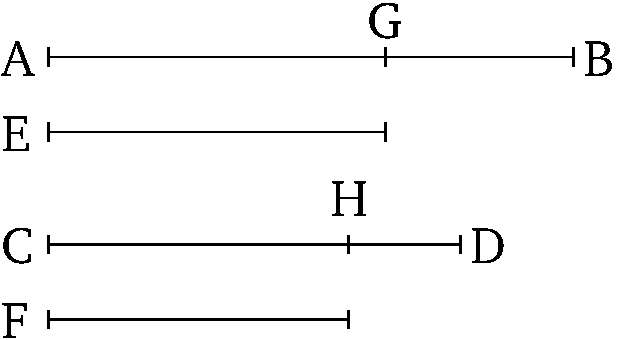
\includegraphics[width=0.8\textwidth]{Book05/fig25e.pdf}}

Let $AB$, $CD$, $E$, and $F$ be four proportional magnitudes, (such that) as
$AB$ (is) to $CD$, so $E$ (is) to $F$. And let $AB$ be the greatest of them, and $F$ the least. I say that $AB$ and $F$ is greater than $CD$ and $E$.

For let $AG$ be made equal to $E$, and $CH$ equal to $F$.

\mbox{[}In fact,] since as $AB$ is to $CD$, so $E$ (is) to $F$, and $E$ (is) equal to $AG$, and
$F$ to $CH$,  thus as $AB$ is to $CD$, so $AG$ (is) to $CH$. And since the whole
$AB$ is to the whole $CD$ as the (part) taken away $AG$ (is) to the
(part) taken away $CH$, thus the remainder $GB$ will also be to the
remainder $HD$ as the whole $AB$ (is) to the whole $CD$ [Prop.~5.19]. And $AB$ (is) greater than $CD$.
Thus, $GB$ (is) also greater than $HD$. And since $AG$ is equal to $E$, and $CH$
to $F$, thus $AG$ and $F$ is equal to $CH$ and $E$. And [since] if [equal (magnitudes)
are added to unequal (magnitudes then) the wholes are unequal, thus if] $AG$ and $F$ are added to $GB$, and $CH$ and
$E$ to $HD$---$GB$ and
$HD$ being unequal, and $GB$ greater---it is inferred that $AB$ and $F$ (is) greater than $CD$ and $E$.

Thus, if four magnitudes are proportional, (then) the (sum of the)
largest  and the smallest of them is greater than the (sum of the) remaining two (magnitudes). (Which is) the very thing it was required to show.}
\end{Parallel}
{\footnotesize \noindent$^\dag$ In modern notation, this proposition
reads that if $\alpha:\beta::\gamma:\delta$, and $\alpha$ is the greatest and $\delta$ the least, then $\alpha+\delta>\beta+\gamma$.}

\newpage~\thispagestyle{empty}
